\documentclass[a4paper]{article}
\setcounter{tocdepth}{3}
\setcounter{secnumdepth}{3}
\usepackage{a4wide,amssymb,epsfig,latexsym,multicol,array,hhline,fancyhdr}
\usepackage{titlesec}
\usepackage{listings}
\usepackage{imakeidx}
\usepackage{tocloft}
\titleformat{\section}{\normalfont\bfseries}{\thesection}{1em}{}
\titleformat{\subsection}{\normalfont\bfseries}{\thesubsection}{1em}{}
\titleformat{\subsubsection}{\normalfont\bfseries}{\thesubsubsection}{1em}{}
\usepackage{verbatim}
\usepackage{longtable}
\usepackage{vntex}
\usepackage{amsmath}
%\usepackage{makecell}
\usepackage{lastpage}
\usepackage[lined,boxed,commentsnumbered]{algorithm2e}
\usepackage{enumerate}
\usepackage{color}
\usepackage{graphicx}							% Standard graphics package
\usepackage{array}
\usepackage{booktabs}
\usepackage{tabularx, caption}
\usepackage{multirow}
\usepackage{multicol}
\usepackage{rotating}
\usepackage{graphics}
\usepackage[table]{xcolor}
\usepackage{geometry}
\usepackage{setspace}
\usepackage{epsfig}
\usepackage{tikz}
\usepackage{cases}
\usetikzlibrary{arrows,snakes,backgrounds}
\usepackage{hyperref}
\hypersetup{urlcolor=blue,linkcolor=black,citecolor=black,colorlinks=true} 
%\usepackage{pstcol} 								% PSTricks with the standard color package

\newtheorem{theorem}{{\bf Theorem}}
\newtheorem{property}{{\bf Property}}
\newtheorem{proposition}{{\bf Proposition}}
\newtheorem{corollary}[proposition]{{\bf Corollary}}
\newtheorem{lemma}[proposition]{{\bf Lemma}}

\AtBeginDocument{\renewcommand*\contentsname{Contents}}
\AtBeginDocument{\renewcommand*\refname{References}}
%\usepackage{fancyhdr}
\setlength{\headheight}{40pt}
\pagestyle{fancy}
\fancyhead{} % clear all header fields
\fancyhead[L]{
 \begin{tabular}{rl}
    \begin{picture}(25,15)(0,0)
    \put(0,-8){
\includegraphics[width=8mm, height=8mm]{hcmut.png}}
    %\put(0,-8){\epsfig{width=10mm,figure=hcmut.eps}}
   \end{picture}&
	%
\includegraphics[width=8mm, height=8mm]{hcmut.png} & %
	\begin{tabular}{l}
		\textbf{\bf \ttfamily ĐẠI HỌC BÁCH KHOA - ĐẠI HỌC QUỐC GIA TPHCM}\\
		\textbf{\bf \ttfamily KHOA KHOA HỌC VÀ KỸ THUẬT MÁY TÍNH}
	\end{tabular} 	
 \end{tabular}
}
\fancyhead[R]{
	\begin{tabular}{l}
		\tiny \bf \\
		\tiny \bf 
	\end{tabular}  }
\fancyfoot{} % clear all footer fields
\fancyfoot[L]{\scriptsize \ttfamily BÀI TẬP LỚN CÔNG NGHỆ PHẦN MỀM - HK 231}
\fancyfoot[R]{\scriptsize \ttfamily Trang {\thepage}/\pageref{LastPage}}
\renewcommand{\headrulewidth}{0.3pt}
\renewcommand{\footrulewidth}{0.3pt}


%%%
\setcounter{secnumdepth}{3}
\setcounter{tocdepth}{3}

\makeatletter
\newcounter {subsubsubsection}[subsubsection]
\renewcommand\thesubsubsubsection{\thesubsubsection .\@alph\c@subsubsubsection}
\newcommand\subsubsubsection{\@startsection{subsubsubsection}{4}{\z@}%
                                     {-3.25ex\@plus -1ex \@minus -.2ex}%
                                     {1.5ex \@plus .2ex}%
                                     {\normalfont\normalsize\bfseries}}
\newcommand*\l@subsubsubsection{\@dottedtocline{3}{10.0em}{4.1em}}
\newcommand*{\subsubsubsectionmark}[1]{}
\setcounter{secnumdepth}{4}

\makeatother



\begin{document}
\begin{titlepage}
\begin{center}
\textbf{ ĐẠI HỌC QUỐC GIA THÀNH PHỐ HỒ CHÍ MINH \\
ĐẠI HỌC BÁCH KHOA  \\
KHOA KHOA HỌC VÀ KỸ THUẬT MÁY TÍNH }\\
\end{center}

\vspace{1cm}

\begin{figure}[h!]
\begin{center}

\includegraphics[width=3cm]{hcmut.png}
\end{center}
\end{figure}

\begin{center}
\begin{tabular}{c}
\multicolumn{1}{l}{\textbf{{\Large CÔNG NGHỆ PHẦN MỀM (CO3001)}}}\\
~~\\
\hline
\\
\multicolumn{1}{l}{\textbf{{\Large BÁO CÁO}}}\\
\\
 \textbf{{\Huge Hệ thống in thông minh}}  \\

\textbf{{\Huge  dành cho sinh viên }}
\\
\textbf{{\Huge tại Trường đại học Bách Khoa}}
\\
\hline
\end{tabular}
\end{center}

\vspace{3cm}

\begin{table}[h]
\begin{tabular}{rll}
\hspace{5cm}
\textcolor{blue}{\textbf{GVHD:}} & \textbf{Phan Trung Hiếu} & \\
\textcolor{blue}{\textbf{Sinh viên:}} & \textbf{Vũ Linh Cường} & - \textbf{2110890} \\
 & \textbf{Nguyễn Sỹ Dương} & - \textbf{2113097} \\
 & \textbf{Vũ Lâm Hoàng Đại} & - \textbf{2110992} \\
 & \textbf{Phan Đức Đạt} & - \textbf{2113152} \\
 & \textbf{Lê Trung Hiếu} & - \textbf{2110168} \\
 & \textbf{Lại Nguyễn Tuấn Khanh} & - \textbf{2110250} \\
 & \textbf{Nguyễn Ngọc Quý} & - \textbf{2114605} \\
\end{tabular}
\end{table}

\begin{center}
{\footnotesize Thành phố Hồ Chí Minh , 2023}
\end{center}
\end{titlepage}

\newpage
\renewcommand{\contentsname}{Mục lục}
\tableofcontents
\newpage

\title{Task 1}
\section{Bảng phân công nhiệm vụ}
\newcolumntype{M}[1]{>{\centering\arraybackslash}m{#1}}

\begin{table}[h!]
\centering
\begin{tabular}{|c|M{4cm}|p{8cm}|}
\hline
\textbf{STT} & \textbf{Họ và Tên} & \textbf{Công việc được giao} \\
\hline
1 & Vũ Linh Cường & Hiện thực api SPSO \\
& & Vẽ class erd/eerd + thiết kế cơ sở dữ liệu \\
\hline
2 & Nguyễn Sỹ Dương & Chỉnh sửa figma \\
& & Chỉnh sửa báo cáo \\
& & Hiện thực task 4.1 và 4.2 \\
\hline
3 & Vũ Lâm Hoàng Đại & Hiện thực phần conduct test và document the feedback from testers của task 4.3. \\
& & Thiết kế giao diện cho hệ thống + xử lý tất cả yêu cầu chức năng người dùng trên reactjs. \\
\hline
4 & Phan Đức Đạt & Hiện thực + viết báo cáo: task 1; task 2,3: phần buy more page \\
& & Chỉnh sửa, thiết kế Diagrams phần Buy more page \\
\hline
5 & Lê Trung Hiếu & Hiện thực api student \\
& & Vẽ class erd/eerd + thiết kế cơ sở dữ liệu. \\
\hline
6 & Lại Nguyễn Tuấn Khanh & Hiện thực +viết báo cáo: task 1; task 2,3: phần print \\
& & Hỗ trợ BE: Hiện thực api phần Print, thiết kế Database \\
& & Chỉnh sửa, thiết kế Diagrams phần Print \\
\hline
7 & Nguyễn Ngọc Quý & Hiện thực phần define test strategy task 4.3 \\
& & Hiện thực +viết báo cáo: task 1; task 2,3: phần login; task 3.1 phần: quản lý API. \\
& & Thiết kế giao diện trang web. (figma) \\
& & Hỗ trợ FE : Thiết kế và chỉnh sửa giao diện hệ thống trên reactjs. \\
\hline
\end{tabular}
\end{table}
\newpage
\section{Tìm hiểu yêu cầu}
\subsection{Lời mở đầu}
Câu chuyện về dịch vụ in thông minh cho sinh viên tại trường Đại học Bách khoa Thành phố Hồ Chí Minh bắt đầu khi chúng tôi nhận ra sự cần thiết của nó ở môi trường học tập bận rộn tại trường. Vì sinh viên sẽ học ở các tòa trong trường nên rõ ràng họ sẽ cần một dịch vụ in thật hiện đại và đáng tin cậy. Đó cũng là khi chúng tôi tạo ra HCMUT-SSPS. Dịch vụ in này không chỉ đơn thuần là in một văn bản, mà nó còn là một nền tảng hoàn chỉnh, được thiết kế để thỏa mãn các nhu cầu khác nhau của sinh viên trong trường. Dịch vụ in này không chỉ đơn giản hóa quá trình in tài liệu mà còn mở rộng khả năng quản lí tài nguyên máy in, giám sát việc sử dụng và tạo môi trường cho việc giao dịch được "mượt mà" hơn. Với HCMUT-SSPS, sinh viên từ giờ sẽ có một cổng thông tin thân thiện để in tài liệu học thuật, bài tập và các loại tài liệu khác trong khi trường sẽ tạo ra lợi nhuận từ việc quản lí và kiểm soát quá trình in ấn một cách hiệu quả.
    \subsection{Các stakeholders liên quan và nhu cầu}
    \begin{enumerate}
        \item {\textbf{Sinh viên}}
             \begin{itemize}
                 \item Có thể in tài liệu.
                 \item Có thể mua trang để in tài liệu và lịch sử giao dịch.
                 \item Xem lịch sử in ấn.
             \end{itemize}
        \item {\textbf{Sinh viên Printing Service Officers (SPSO)}}
             \begin{itemize}
             \item Quản lý các thông tin về các thông số in mà sinh viên được dùng.
                 \item Quản lý các máy in bao gồm thêm, xóa, điều chỉnh thông tin máy in.
                 \item Xem và quản lý lịch sử in của sinh viên.
                 \item Thống kê lịch sử in theo khoảng thời gian mong muốn.
             \end{itemize}
        \item {\textbf{HCMUT\_SSO}}
             \begin{itemize}
                \item Chịu trách nhiệm về triển khai, cấu hình và duy trì HCMUT\_SSO.
                \item Quản lý các tính năng và cấu hình liên quan đến đăng nhập và xác thực người dùng.
                \item Liên kết với bên cung cấp CAS để cung cấp các dịch vụ đăng nhập chung cho các ứng dụng khác nhau, bao gồm HCMUT-SSPS.
             \end{itemize}
             \item {\textbf{CAS (Central Authentication Service)}}
             \begin{itemize}
                \item Cung cấp dịch vụ xác thực trung tâm, giúp quản lý quá trình đăng nhập và xác thực người dùng một cách an toàn và hiệu quả.
                \item Theo dõi và quản lý phiên làm việc của người dùng để đảm bảo tính bảo mật và ngăn chặn các mối quan nguy hiểm.
             \end{itemize}
         \item {\textbf{IT Department }}
         \begin{itemize}
            \item Mở rộng dịch vụ khi nhu cầu sử dụng tăng lên.
             \item Hỗ trợ và bảo trì hệ thống, cơ sở hạ tầng kĩ thuật.
             \end{itemize}
         \item {\textbf{Online Payment System Providers}}
         \begin{itemize}
             \item Tích hợp với hệ thống in ấn.
             \item Yều câu hệ thống truy xuất cơ bản.
         \end{itemize}
    \end{enumerate}



    
    \subsection{Kỳ vọng của Stakeholder}
        \begin{enumerate}
        \item {\textbf{Sinh viên}}
            \begin{itemize}
                \item Dịch vụ in ấn với mức giá tốt và tiết kiệm thời gian.
                \item Nhận được hỗ trợ nhanh chóng, linh hoạt khi gặp vấn đề liên quan đến in ấn.
                \item Có một hệ thống in đầy đủ, bao gồm tùy chọn in tùy chỉnh như kích thước giấy, số trang (của tệp) cần in, in một mặt / hai mặt, và số bản sao.
                \item Nhận được thông báo khi còn lại ít số trang in.
            \end{itemize}
        \item {\textbf{Student Printing Service Officers (SPSO)}}
            \begin{itemize}
                \item Yêu cầu các tùy chọn cấu hình hệ thống nâng cao, như thay đổi số trang mặc định, ngày mà hệ thống sẽ đặt số trang mặc định cho tất cả sinh viên, các loại tệp được phép mà hệ thống chấp nhận.
                \item Đưa ra quyết định dựa trên dữ liệu thông qua việc truy cập vào các bản ghi và báo cáo.
            \end{itemize}
        % \item {\textbf{HCMUT Administration}}
        %     \begin{itemize}
        %         \item Reliable and cost-effective printing service.
        %         \item Reports on printing usage for budgeting purposes.
        %         \item Required advanced system control every SPSO station.
        %     \end{itemize}
            \item {\textbf{HCMUT\_SSO }}
            \begin{itemize}
                \item Quản lí tài khoản người dùng.
                \item Xác thực tài khoản người dùng.
                \item Liên kết với Đại học Bách Khoa Thành phố Hồ Chí Minh để lấy thông tin về tài khoản người dùng.
            \end{itemize}
        \item {\textbf{IT Department} }
            \begin{itemize}
                \item Nhận báo cáo khi trạm dịch vụ in (SPSO) cần sửa chữa.
                \item Truy cập các chỉ số hiệu suất và đối phó với các vấn đề tiềm ẩn trước khi ảnh hưởng đến người dùng.
            \end{itemize}
        \item {\textbf{Online Payment Providers} }
            \begin{itemize}
                \item Thanh toán tuân thủ các tiêu chuẩn bảo mật.
                \item Có khả năng tạo báo cáo doanh thu.
            \end{itemize}
    \end{enumerate}
        





    \subsection{Lợi ích HCMUT-SSPS mang lại cho từng stakeholder}
    \begin{enumerate}
        \item {\textbf{Sinh viên}}
            \begin{itemize}
                \item Tiết kiệm thời gian và công sức khi in tài liệu.
                \item Cung cấp một nền tảng thân thiện với người dùng để in ấn, dễ dàng theo dõi số trang còn lại.
                \item Có nhiều tùy chọn thuận tiện cho việc mua thêm trang in cùng với khả năng kiểm soát chi phí khi mua thêm trang.
            \end{itemize}
        \item {\textbf{Student Printing Service Officers (SPSO)}}
            \begin{itemize}
                \item Có các báo cáo chi tiết hơn giúp tối ưu hóa quyết định và nguồn lực.
                \item Giao diện quản trị dễ sử dụng.
                \item Quản lý hiệu quả dịch vụ in ấn.
            \end{itemize}
        % \item {\textbf{HCMUT Administration}}
        %     \begin{itemize}
        %         \item Enhances data security and compliance, reducing potential risks.
        %         \item Data-driven decisions for resource allocation.
        %     \end{itemize}
            \item {\textbf{HCMUT\_SSO}}
            \begin{itemize}
                \item Nâng cao bảo mật và tuân thủ dữ liệu, giảm thiểu rủi ro tiềm ẩn.
                \item Quyết định dựa trên dữ liệu cho phân phối tài nguyên.
            \end{itemize}
        \item {\textbf{IT Department}}
            \begin{itemize}
                \item Hệ thống vận hành mượt mà.
                \item Giảm thiểu rủi ro bảo mật và thời gian chết của hệ thống.
                \item Tập trung vào hệ thống tự động hóa để giảm chi phí.
            \end{itemize}
        \item {\textbf{Online Payment Providers}}
            \begin{itemize}
                \item Xử lý thanh toán an toàn và hiệu quả.
                \item Hệ thống phù hợp với xu hướng giao dịch trực tuyến hiện nay.
            \end{itemize}
    \end{enumerate}
\subsection{Mô tả tất cả  functional và non-functional requirements từ file mô tả dự án  }
\newcolumntype{s}{>{\columncolor[HTML]{AAACED}} p{3cm}}
 \captionsetup[table]{name=Table}
\subsubsection{Functional requirements}
\begin{enumerate}
    \item {\textbf{Sinh viên}}
        \begin{itemize}
            \item Tạo/ xóa tài khoản.
            \item Tải lên tài liệu, chọn máy in và tùy chỉnh các tùy chọn in ấn dễ dàng.
            \item Theo dõi lịch sử in ấn, kiểm tra số trang còn lại.
            \item Tương tác với Chat Support để giao tiếp với SPSO.
            \item Thay đổi mật khẩu.
    `       \item Thay đổi thông tin cá nhân như số điện thoại, email, địa chỉ.
            \item Theo dõi trạng thái của công việc in ấn như chờ, đang in, đã hoàn thành.
        \end{itemize}
    \item {\textbf{HCMUT\textunderscore SSO}}
        \begin{itemize}
            \item Quản lý phiên đăng nhập.
            \item Xác thực người dùng.
        \end{itemize}
    \item {\textbf{Online payment}}
        \begin{itemize}
            \item Kiểm tra lịch sử thanh toán.
            \item Cho phép người dùng sử dụng nhiều phương thức thanh toán như ngân hàng, thẻ tín dụng, hoặc ví điện tử.
            \item Cập nhật số dư tài khoản và số trang sau khi thanh toán thành công.
        \end{itemize}
    \item {\textbf{SPSO}}
        \begin{itemize}
            \item Nhận yêu cầu in và kiểm tra xem nó có hợp lệ hay không.
            \item Quản lý trạng thái máy in, xem và kiểm tra lịch sử in ấn.
            \item Có thể tùy chỉnh cho máy in.
            \item Có quyền xem thông tin sinh viên để thông báo ngay lập tức nếu có vấn đề.
        \end{itemize}
    \item {\textbf{IT department}}
        \begin{itemize}
            \item Có quyền truy cập vào hệ thống mọi lúc và có khả năng thay đổi các đặc tính của hệ thống.
            \item Đảm bảo hoạt động ổn định của hệ thống và khả năng nâng cấp trong tương lai.
        \end{itemize}
\end{enumerate}
\subsubsection{Non-functional requirements}
\begin{enumerate}
    \item {\textbf{Hiệu suất}}
        \begin{itemize}
            \item Hệ thống phải đảm bảo thời gian phản hồi nhanh khi người dùng yêu cầu in và có khả năng xử lý nhiều yêu cầu (< 10 giây mỗi yêu cầu).
            \item Website của hệ thống sẽ được tải trong 3 giây nếu có ít hơn 1000 người truy cập cùng một lúc.
            \item Tốc độ tải lên tệp trong khoảng 3-5 giây.
        \end{itemize}
    \item {\textbf{Trải nghiệm người dùng}}
        \begin{itemize}
            \item Giao diện có thiết kế hấp dẫn và thẩm mỹ về mặt hình ảnh, màu sắc, bố cục và font chữ.
            \item Giao diện thân thiện với người dùng (Dễ sử dụng với chỉ 5 phút hướng dẫn).
        \end{itemize}
    \item {\textbf{Sự khả dụng}}
        \begin{itemize}
            \item Hệ thống hoạt động 24/7 ngoại trừ thời kỳ bảo trì. Tuy nhiên, việc in chỉ hoạt động từ 6 giờ sáng đến 9 giờ tối.
        \end{itemize} 
    \item {\textbf{Tính tương thích}}
        \begin{itemize}
            \item Tương thích với nhiều trình duyệt web như Google Chrome, Firefox, Microsoft Edge.
        \end{itemize}
    \item {\textbf{Tính mở rộng}}
        \begin{itemize}
            \item Hệ thống phải có khả năng mở rộng đủ để hỗ trợ tất cả sinh viên tại HCMUT trong khi vẫn duy trì hiệu suất tối ưu.
        \end{itemize}
        \item {\textbf{Bảo mật}}
        \begin{itemize}
            \item Có chức năng xác thực và ủy quyền.
        \end{itemize}
\end{enumerate}
\newpage
\subsection{Use-case digram cho toàn bộ hệ thống}
\setlength{\arrayrulewidth}{0.3mm}
\subsubsection{Danh sách actors}
\begin{table}[h]
\centering
\begin{tabular}{|c|l|}
\hline
\rowcolor[HTML]{AAACED}
 Actor ID & Tên actor  \\ \hline
 1 & Người dùng  \\ \hline
 2 & Sinh viên  \\ \hline
 3 & SPSO  \\ \hline
 4 & HCMUT\_SSO  \\ \hline
\end{tabular}
\end{table}
\subsubsection{Use-case diagram}
\begin{figure}[H]
\begin{center}
    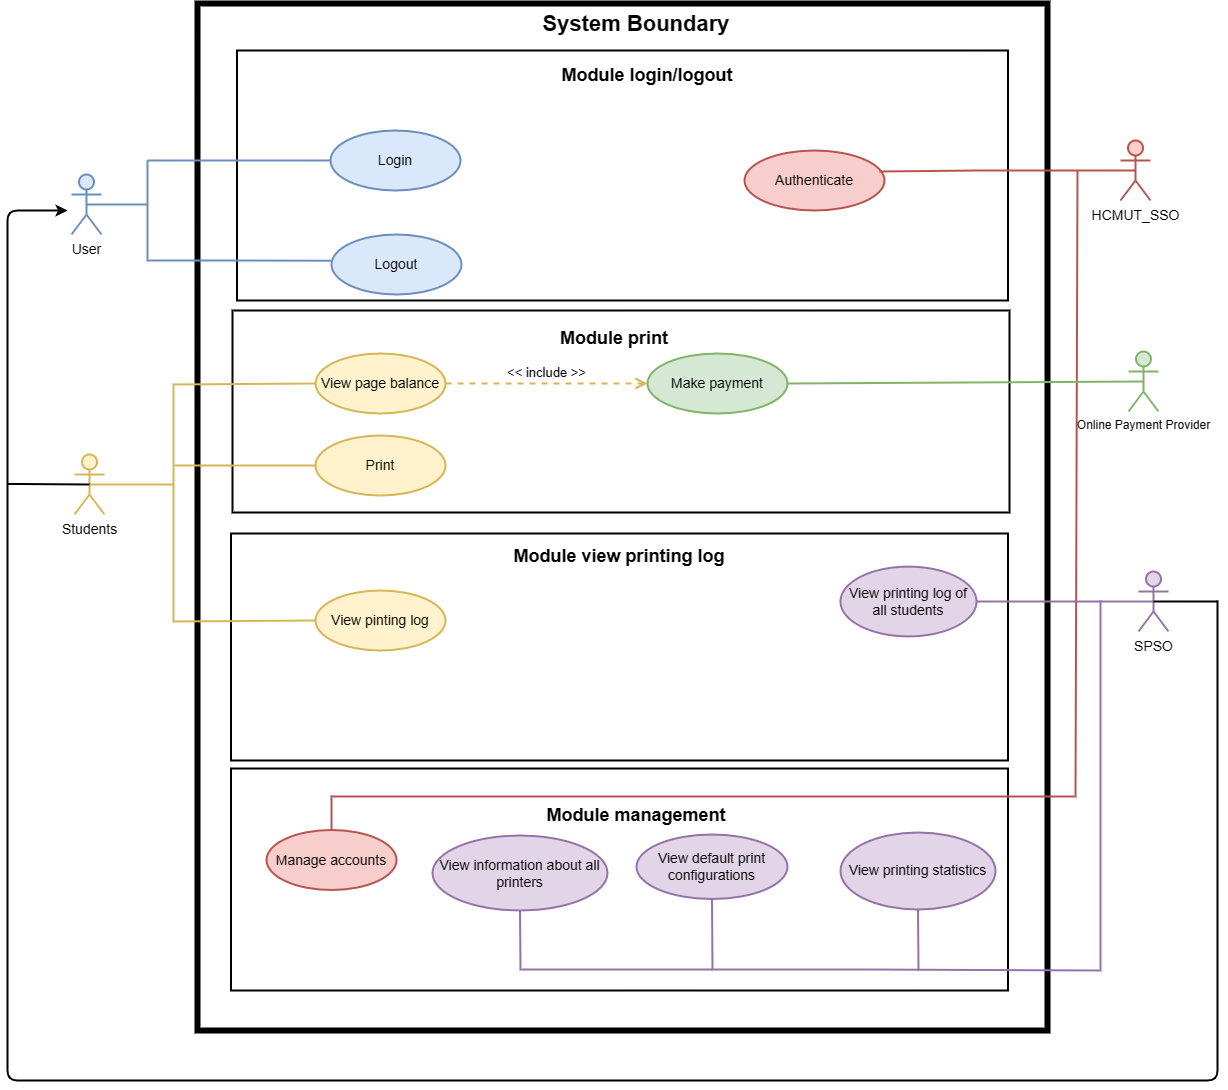
\includegraphics[width=14cm]{picture/Whole_system.drawio (2).png}
    \caption{Use case diagram của hệ thống}
\end{center}
\end{figure}
\subsection{Mô tả use-case}
\subsubsection{Usecase Đăng nhập}
\subsubsubsection{Use-case diagram}
\begin{figure}[h!]
\begin{center}
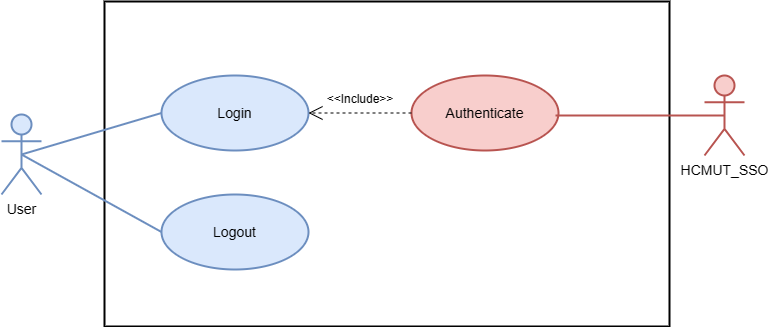
\includegraphics[width=14cm]{picture/use_case_diagram_of_login.drawio (1).png}
\caption{Use case diagram cho module đăng nhập}
\end{center}
\end{figure}
\clearpage
\subsubsubsection{Mô tả use-case diagram theo dạng bảng}
\begin{table}[h]
\centering
\caption{Đăng nhập }
\begin{tabularx}{1.1\textwidth}{|s|X|X|X|}
\hline
 Tên usecase: &  \multicolumn{3}{l|}{Đăng nhập}  \\ \hline
 Tạo bởi: & Nguyễn Ngọc Quý & Cập nhật lần cuối:  &  Nguyễn Ngọc Quý\\ \hline
 Ngày tạo & 22/9/2023  & Ngày cập nhật cuối & 10/11/2023\\ \hline
 Actors: &  \multicolumn{2}{l}{Người dùng} &\\ \hline
 Mô tả: &  \multicolumn{3}{l|}{Cho phép người dùng đăng nhập vào hệ thống.
}  \\ \hline
 Trigger: &  \multicolumn{3}{l|}{Truy cập vào website của SSPS}  \\ \hline
 Tiền điều kiện: &  \multicolumn{3}{l|}
 {\begin{tabular}[t]{@{}l@{}}
1.  Người dùng chưa đăng nhập vào hệ thống. \\
2. Người dùng dùng có tài khoản trên ứng dụng.\\
3. Thiết bị của họ có kết nối mạng.\\
\end{tabular}} \\ \hline
 Hậu điều kiện: &  \multicolumn{3}{l|}{Người dùng đăng nhập thành công.} \\ \hline
 Luồng &  \multicolumn{3}{l|}
 {\begin{tabular}[t]{@{}l@{}}
1. Người dùng truy cập website của hệ thống SSPS và yêu cầu đăng nhập \\
2. Hệ thống sẽ hiển thị giao diện đăng nhập thông qua bên HCMUT\_SSO. \\
3. Người dùng nhập tài khoản và mật khẩu đã được cấp bởi nhà trường. \\
4. Người dùng nhấn nút "Đăng nhập".\\
5. Hệ thống kiểm tra thông tin đăng nhập.\\
6. Hệ thống cập nhật lại giao diện theo thông tin của tài khoản Người dùng.\\
\end{tabular}} \\ \hline
 Các luồng khác &  \multicolumn{3}{l|}{\begin{tabular}[t]{@{}l@{}}
\textbf{A1: Tại bước 3}\\
3.1 Người dùng chọn nút "xóa" để xóa những thông tin vừa điền.\\
3.2 Hệ thống sẽ xóa những thông tin do Người dùng đã điền.\\
\end{tabular}}  \\ \hline
 Ngoại lệ &  \multicolumn{3}{l|}{{\begin{tabular}[t]{@{}l@{}}
 \textbf{E1: Tại bước 3}\\
 5.1 Người dùng nhập tài khoản chưa từng tồn tại\\
5.2 Hệ thống hiển thị thông báo "tài khoản chưa từng tồn tại và vui lòng\\ nhập lại."\\
Tiếp tục bước 3 trong Luồng.\\
\textbf{E2: Tại bước 3}\\
 5.1 Người dùng nhập  tài khoản/mật khẩu sai định dạng.\\
5.2 Hệ thống hiển thị thông báo mật khẩu chưa đúng định dạng hợp lệ.\\
Tiếp tục bước 3 trong Luồng.\\
 \textbf{E3: Tại bước 3}\\
%  5.1 Người chưa nhập hay để trống tài khoản/mật khẩu .\\
% 5.2 Hệ thống hiển thị thông báo vui lòng điền đầy đủ thông tin.\\
% Tiếp tục bước 3 trong Luồng.\\
\textbf{E4: Tại bước 5}\\
 5.1 Người dùng nhập tài khoản/ mật khẩu sai.\\
5.2 Hệ thống hiển thị thông báo sai thông tin đăng nhập.\\
Quay lại bước 3 trong Luồng.
 \end{tabular}}}  \\ \hline
 Ghi chú và lỗi &  \multicolumn{3}{l|}{{\begin{tabular}[t]{@{}l@{}}
%  Nếu người dùng hiện đang đăng nhập, sau đó tiếp tục đăng nhập vào hệ thống\\ bằng
% thiết bị khác, thiết bị cũ sẽ không tự động bị đăng xuất
Không
 \end{tabular}}} \\ \hline
\end{tabularx}
\end{table}
\clearpage
\subsubsection{Usecase In}
\subsubsubsection{Use-case diagram}
\begin{figure}[h!]
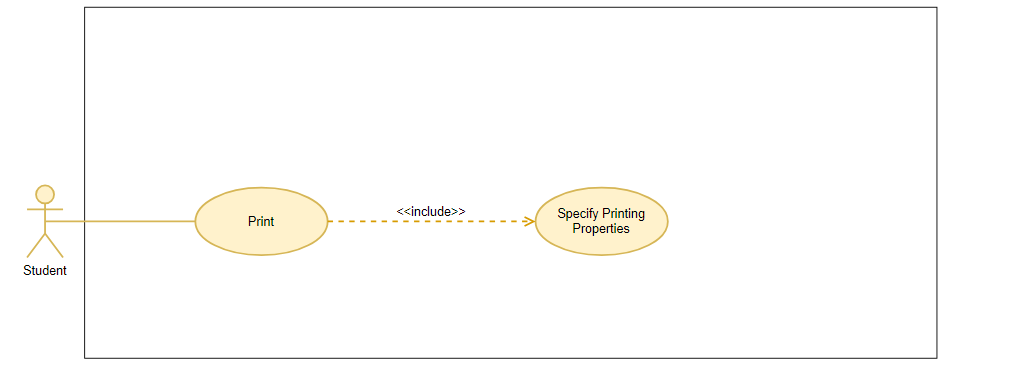
\includegraphics[width=12cm]{picture/use case print.drawio.png}
\caption{Use case diagram cho module print}
\end{figure}

\subsubsubsection{Mô tả use-case diagram theo dạng bảng}

\begin{table}[h!]
\centering
\caption{Thực hiện in use case}
\begin{tabularx}{1.1\textwidth}{|s|X|X|X|}
\hline
 Tên use-case &  \multicolumn{3}{l|}{Thực hiện in}  \\ \hline
 Tạo bởi: & Lại Nguyễn Tuấn Khanh & Cập nhật lần cuối:  &  Lại Nguyễn Tuấn Khanh\\ \hline
 Ngày tạo & 23/9/2023  & Ngày cập nhật cuối & 20/10/2023\\ \hline
 Actors: &  \multicolumn{2}{l}{Sinh viên} &\\ \hline
 Mô tả: & \multicolumn{3}{l|}{Hệ thống giúp Sinh viên in ấn tài liệu.
}  \\ \hline
 Trigger: &  \multicolumn{2}{l}{Chọn "Thực hiện in" trên màn hình giao diện} & \\ \hline
 Tiền điều kiện: &  \multicolumn{3}{l|}
 {\begin{tabular}[t]{@{}l@{}}
 Sinh viên đã đăng nhập vào hệ thống và có quyền sử dụng dịch vụ của SPSO \\
\end{tabular}} \\ \hline

 Hậu điều kiện: &  \multicolumn{2}{l}{Sinh viên thực hiện in ấn tài liệu thành công} &\\ \hline
 Luồng &  \multicolumn{3}{l|}
 {\begin{tabular}[t]{@{}l@{}}
1. Sinh viên chọn "Thực hiện in"\\
2. Sinh viên tiến hành chọn files và chọn máy in.\\
3. Sinh viên hoàn tất thao tác chọn files và máy in.\\
4. Sinh viên chọn các thông số tùy chỉnh.\\
5. Sinh viên xác nhận in\\
6. Hệ thống kiểm tra và lưu lại các thao tác của sinh viên\\
7. Hệ thống bắt đầu tiến hành in\\
\end{tabular}} \\ \hline
 Các luồng khác &  \multicolumn{2}{l}{\begin{tabular}[t]{@{}l@{}}
\end{tabular}}
 & \\ \hline
 Ngoại lệ &  \multicolumn{3}{l|}{\begin{tabular}[t]{@{}l@{}}
E1: \textbf{Tại bước 6:} Sinh viên không còn đủ số lượng trang để in theo yêu cầu\\
1. Hệ thống thông báo "Bạn không còn đủ số lượng trang để in".\\
2. Hệ thống gợi ý Sinh viên mua thêm trang in.\\
3. Sinh viên chọn mua thêm trang in hoặc không.\\
3.1 Nếu Sinh viên không mua, hệ thống trở về màn hình giao diện in ấn\\
3.2 Nếu Sinh viên mua, hệ thống chuyển đến màn hình giao diện mua trang và\\ thanh toán, sau đó thực hiện in.\\
\end{tabular}}  \\ \hline
 Ghi chú và lỗi & \multicolumn{2}{l}{Không} &\\ \hline
\end{tabularx}
\end{table}

% \begin{table}[h!]
% \centering
% \caption{Cập nhật files use case}
% \begin{tabularx}{1.1\textwidth}{|s|X|X|X|}
% \hline
%  Tên use-case &  \multicolumn{3}{l|}{Cập nhật files}  \\ \hline
%  Tạo bởi: & Lại Nguyễn Tuấn Khanh & Cập nhật lần cuối:  &  Lại Nguyễn Tuấn Khanh\\ \hline
%  Ngày tạo & 23/9/2023  & Ngày cập nhật cuối & 20/10/2023\\ \hline
%  Actors: &  \multicolumn{2}{l}{Sinh viên} &\\ \hline
%  Mô tả: & \multicolumn{3}{l|}{Hệ thống giúp sinh viên cập nhật files tài liệu để in ấn}  \\ \hline
%  Trigger: &  \multicolumn{2}{l}{Chọn "Cập nhật files" trên màn hình giao diện in ấn} & \\ \hline
%  Tiền điều kiện: &  \multicolumn{3}{l|}
%  {\begin{tabular}[t]{@{}l@{}}
% Sinh viên đã đăng nhập vào hệ thống và có quyền sử dụng dịch vụ của SPSO\\
% \end{tabular}} \\ \hline

%  Hậu điều kiện: &  \multicolumn{2}{l}{Sinh viên cập nhật files tài liệu thành công} &\\ \hline
%  Luồng &  \multicolumn{3}{l|}
%  {\begin{tabular}[t]{@{}l@{}}
% 1. Sinh viên chọn "Cập nhật files"\\
% 2. Hệ thống hiển thị màn hình giao diện cập nhật files\\
% 3. Sinh viên chọn files để tải lên hệ thống\\
% 4. Hệ thống lưu lại thao tác của Sinh viên và tải files lên\\
% 5. Hệ thống thông báo "Bạn đã cập nhật files thành công".
% \end{tabular}} \\ \hline
%  Các luồng khác &  \multicolumn{2}{l}{\begin{tabular}[t]{@{}l@{}}
%  A1: \textbf{Tại bước 3:} Sinh viên rời khỏi bước cập nhật files\\
% 1. Sinh viên chọn "Hủy" trên màn hình giao diện cập nhật files\\
% 2. Hệ thống xóa files đã chọn\\
% 3. Hệ thống trở về màn hình giao diện trước\\
% \end{tabular}}
%  & \\ \hline
%  Ngoại lệ &  \multicolumn{3}{l|}{\begin{tabular}[t]{@{}l@{}}
% E1: \textbf{Tại bước 3:} Sinh viên cập nhật files không tương thích\\
% 1. Hệ thống thông báo "Files không tương thích với hệ thống".\\
% 2. Hệ thống trở về màn hình giao diện cập nhật files.\\
% \end{tabular}}  \\ \hline
%  Ghi chú và lỗi &  \multicolumn{2}{l}{Không} &\\ \hline
% \end{tabularx}
% \end{table}
% \newpage


% \begin{table}[h!]
% \centering
% \caption{Chọn máy in use case}
% \begin{tabularx}{1.1\textwidth}{|s|X|X|X|}
% \hline
%  Tên use-case &  \multicolumn{3}{l|}{Chọn máy in}  \\ \hline
%  Tạo bởi: & Lại Nguyễn Tuấn Khanh & Cập nhật lần cuối:  &  Lại Nguyễn Tuấn Khanh\\ \hline
%  Ngày tạo & 23/9/2023  & Ngày cập nhật cuối & 20/10/2023\\ \hline
%  Actors: &  \multicolumn{2}{l}{Sinh viên} &\\ \hline
%  Mô tả: & \multicolumn{3}{l|}{Hệ thống giúp Sinh viên chọn máy in}  \\ \hline
%  Trigger: &  \multicolumn{2}{l}{Chọn "Chọn máy in" trên màn hình giao diện in ấn} & \\ \hline
%  Tiền điều kiện: &  \multicolumn{3}{l|}
%  {\begin{tabular}[t]{@{}l@{}}
% Sinh viên đã đăng nhập vào hệ thống và có quyền sử dụng dịch vụ của SPSO\\
% \end{tabular}} \\ \hline

%  Hậu điều kiện: &  \multicolumn{2}{l}{Sinh viên chọn máy in để in ấn tài liệu thành công} &\\ \hline
%  Luồng &  \multicolumn{3}{l|}
%  {\begin{tabular}[t]{@{}l@{}}
% 1. Sinh viên chọn "Chọn máy in"\\
% 2. Hệ thống hiển thị màn hình giao diện chọn máy in\\
% 3. Sinh viên chọn máy in để sử dụng\\
% 4. Hệ thống lưu lại thao tác của Sinh viên và kiểm tra tình trạng của máy in\\
% 5. Hệ thống thông báo "Chọn máy in thành công".
% \end{tabular}} \\ \hline
%  Các luồng khác &  \multicolumn{2}{l}{\begin{tabular}[t]{@{}l@{}}
%  A1: \textbf{Tại bước 3:} Sinh viên rời khỏi bước chọn máy in\\
% 1. Sinh viên chọn "Hủy" trên màn hình giao diện chọn máy in\\
% 2. Hệ thống xóa máy in đã được chọn.\\
% 3. Hệ thống trở về màn hình giao diện trước.
% \end{tabular}}
%  & \\ \hline
%  Ngoại lệ &  \multicolumn{3}{l|}{\begin{tabular}[t]{@{}l@{}}
% E1: \textbf{Tại bước 3:} Máy in được chọn hiện đang được sử dụng bởi Người dùng khác.\\
% 1. Hệ thống thông báo "Máy in được chọn hiện đang bận. Vui lòng chờ nếu\\ chọn máy in này."\\
% 2. Hệ thống đưa ra 2 lựa chọn cho Sinh viên "Tiếp tục chọn", "Chọn máy in\\ khác"\\
% 2.1 Nếu Sinh viên chọn "Tiếp tục chọn" thì hệ thống thông báo "Chọn
% máy\\ in thành công"\\
% 2.2 Nếu Sinh viên chọn "Chọn máy in khác" thì hệ thống trở về màn hình\\ giao diện chọn máy in\\
% \end{tabular}}  \\ \hline
%  Ghi chú và lỗi &  \multicolumn{2}{l}{Không} &\\ \hline
% \end{tabularx}
% \end{table}

% \newpage

\begin{table}[h!]
\centering
\caption{Xác định thông số tùy chỉnh in ấn use case}
\begin{tabularx}{1.1\textwidth}{|s|X|X|X|}
\hline
 Tên use-case &  \multicolumn{3}{l|}{Xác định thông số tùy chỉnh in ấn}  \\ \hline
 Tạo bởi: & Lại Nguyễn Tuấn Khanh & Cập nhật lần cuối:  &  Lại Nguyễn Tuấn Khanh\\ \hline
 Ngày tạo & 23/9/2023  & Ngày cập nhật cuối & 20/10/2023\\ \hline
 Actors: &  \multicolumn{2}{l}{Sinh viên} &\\ \hline
 Mô tả: & \multicolumn{3}{l|}{Hệ thống giúp Sinh viên xác định thông số tùy chỉnh in ấn}  \\ \hline
 Trigger: &  \multicolumn{3}{l|}{Sinh viên đang thực hiện in}  \\ \hline
 Tiền điều kiện: &  \multicolumn{3}{l|}
 {\begin{tabular}[t]{@{}l@{}}
Sinh viên đã đăng nhập vào hệ thống và có quyền sử dụng dịch vụ của SPSO\\
\end{tabular}} \\ \hline

 Hậu điều kiện: &  \multicolumn{2}{l}{Sinh viên xác định thông số tùy chỉnh in ấn thành công} &\\ \hline
 Luồng &  \multicolumn{3}{l|}
 {\begin{tabular}[t]{@{}l@{}}
1. Hệ thống hiển thị màn hình giao diện các thông số tùy chỉnh in ấn\\
2. Sinh viên chọn, điều chỉnh các thông số tùy chỉnh in ấn\\
3. Hệ thống lưu lại các thông số tùy chỉnh in ấn\\
4. Sinh viên hoàn thao tác.
\end{tabular}} \\ \hline
 Các luồng khác &  \multicolumn{3}{l|}{\begin{tabular}[t]{@{}l@{}}
\end{tabular}}
  \\ \hline
 Ngoại lệ &  \multicolumn{3}{l|}{\begin{tabular}[t]{@{}l@{}}
 Không\\
\end{tabular}}  \\ \hline
Ghi chú và lỗi &  \multicolumn{2}{l}{Không} &\\ \hline
\end{tabularx}
\end{table}

% \newpage 
% \begin{table}[h!]
% \centering
% \caption{Quản lý Files use case}
% \begin{tabularx}{1.1\textwidth}{|s|X|X|X|}
% \hline
%  Tên use-case &  \multicolumn{3}{l|}{Quản lý Files}  \\ \hline
%  Tạo bởi: & Lại Nguyễn Tuấn Khanh & Cập nhật lần cuối:  &  Lại Nguyễn Tuấn Khanh\\ \hline
%  Ngày tạo & 13/11/2023  & Ngày cập nhật cuối & 13/11/2023\\ \hline
%  Actors: &  \multicolumn{2}{l}{Sinh viên} &\\ \hline
%  Mô tả: & \multicolumn{3}{l|}{Hệ thống giúp Sinh viên quản lý files}  \\ \hline
%  Trigger: &  \multicolumn{3}{l|}{Sinh viên bấm chọn "Quản lý Files"}  \\ \hline
%  Tiền điều kiện: &  \multicolumn{3}{l|}
%  {\begin{tabular}[t]{@{}l@{}}
% Sinh viên đã đăng nhập vào hệ thống và có quyền sử dụng dịch vụ của SPSO\\
% \end{tabular}} \\ \hline

%  Hậu điều kiện: &  \multicolumn{2}{l}{Sinh viên tải/xóa files thành công} &\\ \hline
%  Luồng &  \multicolumn{3}{l|}
%  {\begin{tabular}[t]{@{}l@{}}
% 1. Hệ thống hiển thị danh sách files của Sinh viên.\\
% 2. Sinh viên chọn thao tác upload/remove files trên danh sách.\\
% 3. Sinh viên chọn files để upload/remove.\\
% 4. Sinh viên hoàn thành thao tác và xác nhận.\\
% \end{tabular}} \\ \hline
%  Các luồng khác &  \multicolumn{3}{l|}{\begin{tabular}[t]{@{}l@{}}
% \end{tabular}}
%   \\ \hline
%  Ngoại lệ &  \multicolumn{3}{l|}{\begin{tabular}[t]{@{}l@{}}
%  Không\\
% \end{tabular}}  \\ \hline
% Ghi chú và lỗi &  \multicolumn{2}{l}{Không} &\\ \hline
% \end{tabularx}
% \end{table}

% \begin{table}[h!]
% \centering
%     \caption{Tải files vào danh sách use case}
% \begin{tabularx}{1.1\textwidth}{|s|X|X|X|}
% \hline
%  Tên use-case &  \multicolumn{3}{l|}{Quản lý Files}  \\ \hline
%  Tạo bởi: & Lại Nguyễn Tuấn Khanh & Cập nhật lần cuối:  &  Lại Nguyễn Tuấn Khanh\\ \hline
%  Ngày tạo & 13/11/2023  & Ngày cập nhật cuối & 13/11/2023\\ \hline
%  Actors: &  \multicolumn{2}{l}{Sinh viên} &\\ \hline
%  Mô tả: & \multicolumn{3}{l|}{Hệ thống giúp Sinh viên tải files vào danh sách files}  \\ \hline
%  Trigger: &  \multicolumn{3}{l|}{Sinh viên bấm chọn "Upload Files"}  \\ \hline
%  Tiền điều kiện: &  \multicolumn{3}{l|}
%  {\begin{tabular}[t]{@{}l@{}}
% Sinh viên đã đăng nhập vào hệ thống và có quyền sử dụng dịch vụ của SPSO\\
% \end{tabular}} \\ \hline

%  Hậu điều kiện: &  \multicolumn{2}{l}{Sinh viên tải files vào danh sách thành công} &\\ \hline
%  Luồng &  \multicolumn{3}{l|}
%  {\begin{tabular}[t]{@{}l@{}}
% 1. Hệ thống hiển thị các files trên máy tính của Student.\\
% 2. Sinh viên chọn files để tải vào danh sách files.\\
% 3. Sinh viên hoàn tất thao tác tải files vào danh sách files.\\
% 4. Sinh viên hoàn thành thao tác và xác nhận.\\
% \end{tabular}} \\ \hline
%  Các luồng khác &  \multicolumn{3}{l|}{\begin{tabular}[t]{@{}l@{}}
% \end{tabular}}
%   \\ \hline
%  Ngoại lệ &  \multicolumn{3}{l|}{\begin{tabular}[t]{@{}l@{}}
%  Không\\
% \end{tabular}}  \\ \hline
% Ghi chú và lỗi &  \multicolumn{2}{l}{Không} &\\ \hline
% \end{tabularx}
% \end{table}

% \newpage
% \begin{table}[h!]
% \centering
%     \caption{Xóa files khỏi danh sách use case}
% \begin{tabularx}{1.1\textwidth}{|s|X|X|X|}
% \hline
%  Tên use-case &  \multicolumn{3}{l|}{Quản lý Files}  \\ \hline
%  Tạo bởi: & Lại Nguyễn Tuấn Khanh & Cập nhật lần cuối:  &  Lại Nguyễn Tuấn Khanh\\ \hline
%  Ngày tạo & 13/11/2023  & Ngày cập nhật cuối & 13/11/2023\\ \hline
%  Actors: &  \multicolumn{2}{l}{Sinh viên} &\\ \hline
%  Mô tả: & \multicolumn{3}{l|}{Hệ thống giúp Sinh viên xóa files khỏi danh sách files}  \\ \hline
%  Trigger: &  \multicolumn{3}{l|}{Sinh viên bấm chọn "Remove Files"}  \\ \hline
%  Tiền điều kiện: &  \multicolumn{3}{l|}
%  {\begin{tabular}[t]{@{}l@{}}
% Sinh viên đã đăng nhập vào hệ thống và có quyền sử dụng dịch vụ của SPSO\\
% \end{tabular}} \\ \hline

%  Hậu điều kiện: &  \multicolumn{2}{l}{Sinh viên tải files vào danh sách thành công} &\\ \hline
%  Luồng &  \multicolumn{3}{l|}
%  {\begin{tabular}[t]{@{}l@{}}
% 1. Hệ thống hiển thị các files hiện có trong danh sách files của Student.\\
% 2. Student chọn files để xóa khỏi danh sách files.\\
% 3. Student hoàn tất thao tác xóa files khỏi danh sách files.\\
% 4. Student hoàn thành thao tác và xác nhận.\\
% \end{tabular}} \\ \hline
%  Các luồng khác &  \multicolumn{3}{l|}{\begin{tabular}[t]{@{}l@{}}
% \end{tabular}}
%   \\ \hline
%  Ngoại lệ &  \multicolumn{3}{l|}{\begin{tabular}[t]{@{}l@{}}
%  Không\\
% \end{tabular}}  \\ \hline
% Ghi chú và lỗi &  \multicolumn{2}{l}{Không} &\\ \hline
% \end{tabularx}
% \end{table}



% \begin{table}[h!]
% \centering
% \caption{Tính toán và báo cáo các trang in use case}
% \begin{tabularx}{1.1\textwidth}{|s|X|X|X|}
% \hline
%  Tên use-case &  \multicolumn{3}{l|}{Tính toán và báo cáo các trang in}  \\ \hline
%  Tạo bởi: & Lại Nguyễn Tuấn Khanh & Cập nhật lần cuối:  &  Lại Nguyễn Tuấn Khanh\\ \hline
%  Ngày tạo & 24/10/2023  & Ngày cập nhật cuối & 24/10/2023\\ \hline
%  Actors: &  \multicolumn{2}{l}{HCMUT\_SSO} &\\ \hline
%  Mô tả: & \multicolumn{3}{l|}{HCMUT\_SSO tính toán và báo cáo số liệu các trang in}  \\ \hline
%  Trigger: &  \multicolumn{3}{l|}{Sinh viên thực hiện in ấn}  \\ \hline
%  Tiền điều kiện: &  \multicolumn{3}{l|}
%  {\begin{tabular}[t]{@{}l@{}}
% Yêu cầu in ấn của Sinh viên được gửi đi\\
% \end{tabular}} \\ \hline

%  Hậu điều kiện: &  \multicolumn{3}{l|}{Hệ thống tính toán và báo cáo các trang in, cập nhật vào dữ liệu hệ thống} \\ \hline
%  Luồng &  \multicolumn{3}{l|}
%  {\begin{tabular}[t]{@{}l@{}}
% 1. Sinh viên thực hiện việc in ấn\\
% 2. HCMUT\_SSO dựa vào số trang của Sinh viên và tính toán số\\ trang còn lại sau khi in\\
% 3. HCMUT\_SSO chấp nhận yêu cầu in ấn hợp lệ\\
% 4. Hệ thống cập nhật thông tin các trang in ấn và số trang của Sinh viên lên\\ cơ sở dữ liệu.\\
% \end{tabular}} \\ \hline
%  Các luồng khác &  \multicolumn{3}{l|}{\begin{tabular}[t]{@{}l@{}}
%  A1: \textbf{Tại bước 2:} Số trang còn lại của Sinh viên không hợp lệ (<0)\\
% 1. HCMUT\_SSO không chấp nhận yêu cầu in ấn\\
% 2. Hệ thống thông báo "Bạn không còn đủ số lượng giấy để in"\\
% \end{tabular}}
%   \\ \hline
%  Ngoại lệ &  \multicolumn{3}{l|}{\begin{tabular}[t]{@{}l@{}}
%  Không\\
% \end{tabular}}  \\ \hline
% Ghi chú và lỗi &  \multicolumn{2}{l}{Không} &\\ \hline
% \end{tabularx}
% \end{table}

% \begin{table}[h!]
% \centering
% \caption{Kết nối máy in use case}
% \begin{tabularx}{1.1\textwidth}{|s|X|X|X|}
% \hline
%  Tên use-case &  \multicolumn{3}{l|}{Kết nối máy in}  \\ \hline
%  Tạo bởi: & Lại Nguyễn Tuấn Khanh & Cập nhật lần cuối:  &  Lại Nguyễn Tuấn Khanh\\ \hline
%  Ngày tạo & 24/10/2023  & Ngày cập nhật cuối & 24/10/2023\\ \hline
%  Actors: &  \multicolumn{2}{l}{HCMUT\_SSO} &\\ \hline
%  Mô tả: & \multicolumn{3}{l|}{HCMUT\_SSO thực hiện kết nối với máy in được chọn để in}  \\ \hline
%  Trigger: &  \multicolumn{3}{l|}{Sinh viên thực hiện yêu cầu in ấn và được HCMUT\_SSO chấp nhận}  \\ \hline
%  Tiền điều kiện: &  \multicolumn{3}{l|}
%  {\begin{tabular}[t]{@{}l@{}}
% Yêu cầu in ấn của Sinh viên được gửi đi\\
% \end{tabular}} \\ \hline

%  Hậu điều kiện: &  \multicolumn{3}{l|}{Hệ thống kết nối với máy in để in ấn thành công} \\ \hline
%  Luồng &  \multicolumn{3}{l|}
%  {\begin{tabular}[t]{@{}l@{}}
% 1. HCMUT\_SSO chấp nhận yêu cầu in ấn\\
% 2. HCMUT\_SSO kết nối với máy in được chọn\\
% 3. HCMUT\_SSO thực hiện in ấn thông qua máy in được chọn\\
% \end{tabular}} \\ \hline
%  Các luồng khác &  \multicolumn{3}{l|}{\begin{tabular}[t]{@{}l@{}}
%  Không\\
% \end{tabular}}
%   \\ \hline
%  Ngoại lệ &  \multicolumn{3}{l|}{\begin{tabular}[t]{@{}l@{}}
%  Không\\
% \end{tabular}}  \\ \hline
% Ghi chú và lỗi &  \multicolumn{2}{l}{Không} &\\ \hline
% \end{tabularx}
% \end{table}

% \newpage
\newpage
\subsubsection{Usecase Xem số dư trang}
\subsubsubsection{Use-case diagram}
\begin{figure}[h!]
\begin{center}
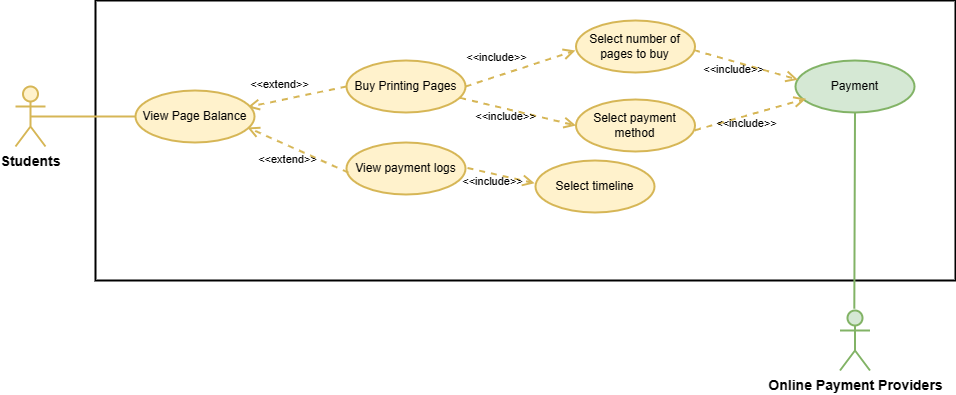
\includegraphics[width=14cm]{picture/Usecasse_of_viewpage.drawio.png}
\caption{Use case diagram cho module xem số dư trang}
\end{center}
\end{figure}
% \newpage
\clearpage
\subsubsubsection{Use case description}
\begin{table}[h!]
\centering
\caption{Mua trang in use case}
\begin{tabularx}{1.1\textwidth}{|s|X|X|X|}
\hline
 Tên use-case &  \multicolumn{3}{l|}{Mua trang in}  \\ \hline
 Tạo bởi: & Phan Đức Đạt  & Cập nhật lần cuối: &  Phan Đức Đạt\\ \hline
 Ngày tạo & 25/9/2023  & Ngày cập nhật cuối & 21/10/2023\\ \hline
 Actors: &  \multicolumn{3}{l|}{Sinh viên} \\ \hline
 Mô tả: &  \multicolumn{3}{l|}{Hệ thống giúp Sinh viên mua thêm trang in.} \\ \hline
 Trigger: &  \multicolumn{3}{l|}{Chọn "Mua trang in" trên màn hình giao diện xem số trang in dư.} \\ \hline
 Tiền điều kiện: &  \multicolumn{3}{l|}{Sinh viên đã đăng nhập vào hệ thống và có quyền sử dụng dịch vụ.} \\ \hline
 Hậu điều kiện: &  \multicolumn{3}{l|}{Sinh viên thanh toán thành công và được cập nhật số trang in.}\\ \hline
 Luồng &  \multicolumn{3}{l|}
 {\begin{tabular}[t]{@{}l@{}}
1. Sinh viên chọn "Mua trang in".\\
2. Hệ thống hiển thị giao diện để chọn số trang cần mua.\\
3. Sinh viên chọn số trang mình cần mua thêm.\\
4. Sinh viên chọn phương thức thanh toán.\\
5. Hệ thống mở ra website tương ứng với phương thức đã chọn.\\
6. Studens tiến hành thanh toán.\\
7. Online payment providers xác thực thanh toán và hệ thống cập nhật số \\
trang in cho Sinh viên.\\
\end{tabular}} \\ \hline
Các luồng khác &  \multicolumn{3}{l|}{\begin{tabular}[t]{@{}l@{}}
\textbf{Tại bước 4:} Sinh viên có thể quay lại để chọn phương thức thanh toán khác.\\
1. Sinh viên chọn nút "quay lại" trên cửa sổ giao diện.\\
2. Hệ thống sẽ chuyển về bước chọn phương thức thanh toán.\\
\end{tabular}}  \\ \hline
Ngoại lệ &  \multicolumn{3}{l|}{\begin{tabular}[t]{@{}l@{}}
 \textbf{Tại bước 5}: Số dư trong tài khoản không đủ.\\
 1. Hệ thống sẽ thông báo cho Sinh viên biết số dư không đủ.\\
 2. Chuyển về bước 4 để chọn một phương thức thanh toán khác.\\ 
\end{tabular}}  \\ \hline
 Ghi chú và lỗi &  \multicolumn{2}{l}{Không} &\\ \hline
\end{tabularx}
\end{table}
\newpage
\begin{table}[h!]
\centering
\caption{Xem lịch sử giao dịch use case}
\begin{tabularx}{1.1\textwidth}{|s|X|X|X|}
\hline
 Tên use-case &  \multicolumn{3}{l|}{Xem lịch sử giao dịch}  \\ \hline
 Tạo bởi: & Phan Đức Đạt  & Cập nhật lần cuối: &  Phan Đức Đạt\\ \hline
 Ngày tạo & 25/9/2023  & Ngày cập nhật cuối & 21/10/2023\\ \hline
 Actors: &  \multicolumn{3}{l|}{Sinh viên, Online Payment Providers} \\ \hline
 Mô tả: &  \multicolumn{3}{l|}{Hệ thống giúp Sinh viên xem lại lịch sử giao dịch.} \\ \hline
 Trigger: &  \multicolumn{3}{l|}{Chọn "Lịch sử giao dịch" trên màn hình giao diện" xem số trang in dư.} \\ \hline
 Tiền điều kiện: &  \multicolumn{3}{l|}{Sinh viên đã đăng nhập vào hệ thống và có quyền sử dụng dịch vụ.} \\ \hline
 Hậu điều kiện: &  \multicolumn{3}{l|}{Sinh viên xem lại lịch sử giao dịch thành công.}\\ \hline
 Luồng &  \multicolumn{3}{l|}
 {\begin{tabular}[t]{@{}l@{}}
1. Sinh viên chọn "Xem lịch sử giao dịch".  \\
2. Hệ thống hiển thị giao diện để chọn mốc thời gian.\\
3. Sinh viên chọn mốc thời gian cần xem. \\
4. Hệ thống hiển thị lịch sử giao dịch trong mốc thời gian tương ứng.\\
\end{tabular}} \\ \hline
 Các luồng khác &  \multicolumn{2}{l}{Không} & \\ \hline
Ngoại lệ &  \multicolumn{3}{l|}{\begin{tabular}[t]{@{}l@{}}
 \textbf{Tại bước 4}: Không thể chọn mốc thời gian vượt quá thời gian thực.\\
 1. Hệ thống thông báo mốc thời gian đã chọn vượt quá thời gian thực.\\
 2. Hệ thống yêu cầu Sinh viên chọn lại mốc thời gian.\\ 
\end{tabular}}  \\ \hline
 Ghi chú và lỗi &  \multicolumn{2}{l}{Không} &\\ \hline
\end{tabularx}
\end{table}

\begin{table}[h!]
\centering
\caption{Xem số trang in dư use case}
\begin{tabularx}{1.1\textwidth}{|s|X|X|X|}
\hline
 Tên use-case &  \multicolumn{3}{l|}{Xem số trang in dư}  \\ \hline
 Tạo bởi: & Phan Đức Đạt  & Cập nhật lần cuối: &  Phan Đức Đạt\\ \hline
 Ngày tạo & 25/9/2023  & Ngày cập nhật cuối & 21/10/2023\\ \hline
 Actors: &  \multicolumn{3}{l|}{Sinh viên} \\ \hline
 Mô tả: &  \multicolumn{3}{l|}{Sinh viên có thể xem số trang in dư của họ.} \\ \hline
 Tiền điều kiện: &  \multicolumn{3}{l|}{Sinh viên đã đăng nhập vào hệ thống và có quyền sử dụng dịch vụ.} \\ \hline
 Hậu điều kiện: &  \multicolumn{3}{l|}{Sinh viên xem số trang in dư thành công. }\\ \hline
 Luồng &  \multicolumn{3}{l|}
 {\begin{tabular}[t]{@{}l@{}}
1. Sinh viên có thể xem số trang in dư của họ ở góc trên bên phải của giao diện. \\
\end{tabular}} \\ \hline
 Các luồng khác &  \multicolumn{2}{l}{Không} & \\ \hline
Ngoại lệ &  \multicolumn{3}{l|}{\begin{tabular}[t]{@{}l@{}}
Không\\
\end{tabular}}  \\ \hline
 Ghi chú và lỗi &  \multicolumn{2}{l}{Không} &\\ \hline
\end{tabularx}
\end{table}
\newpage
% //^^^^^^^^^^^^^^^^^^^^^^^^^^^^^^^^^^^^^^^^^^^^^^^^^^^
% \section{System modeling}
\title{Task 2}
\section{Mô hình hóa hệ thống}
\subsection{Activity Diagram}
\subsubsection{In}
\begin{figure}[h!]
\begin{center}
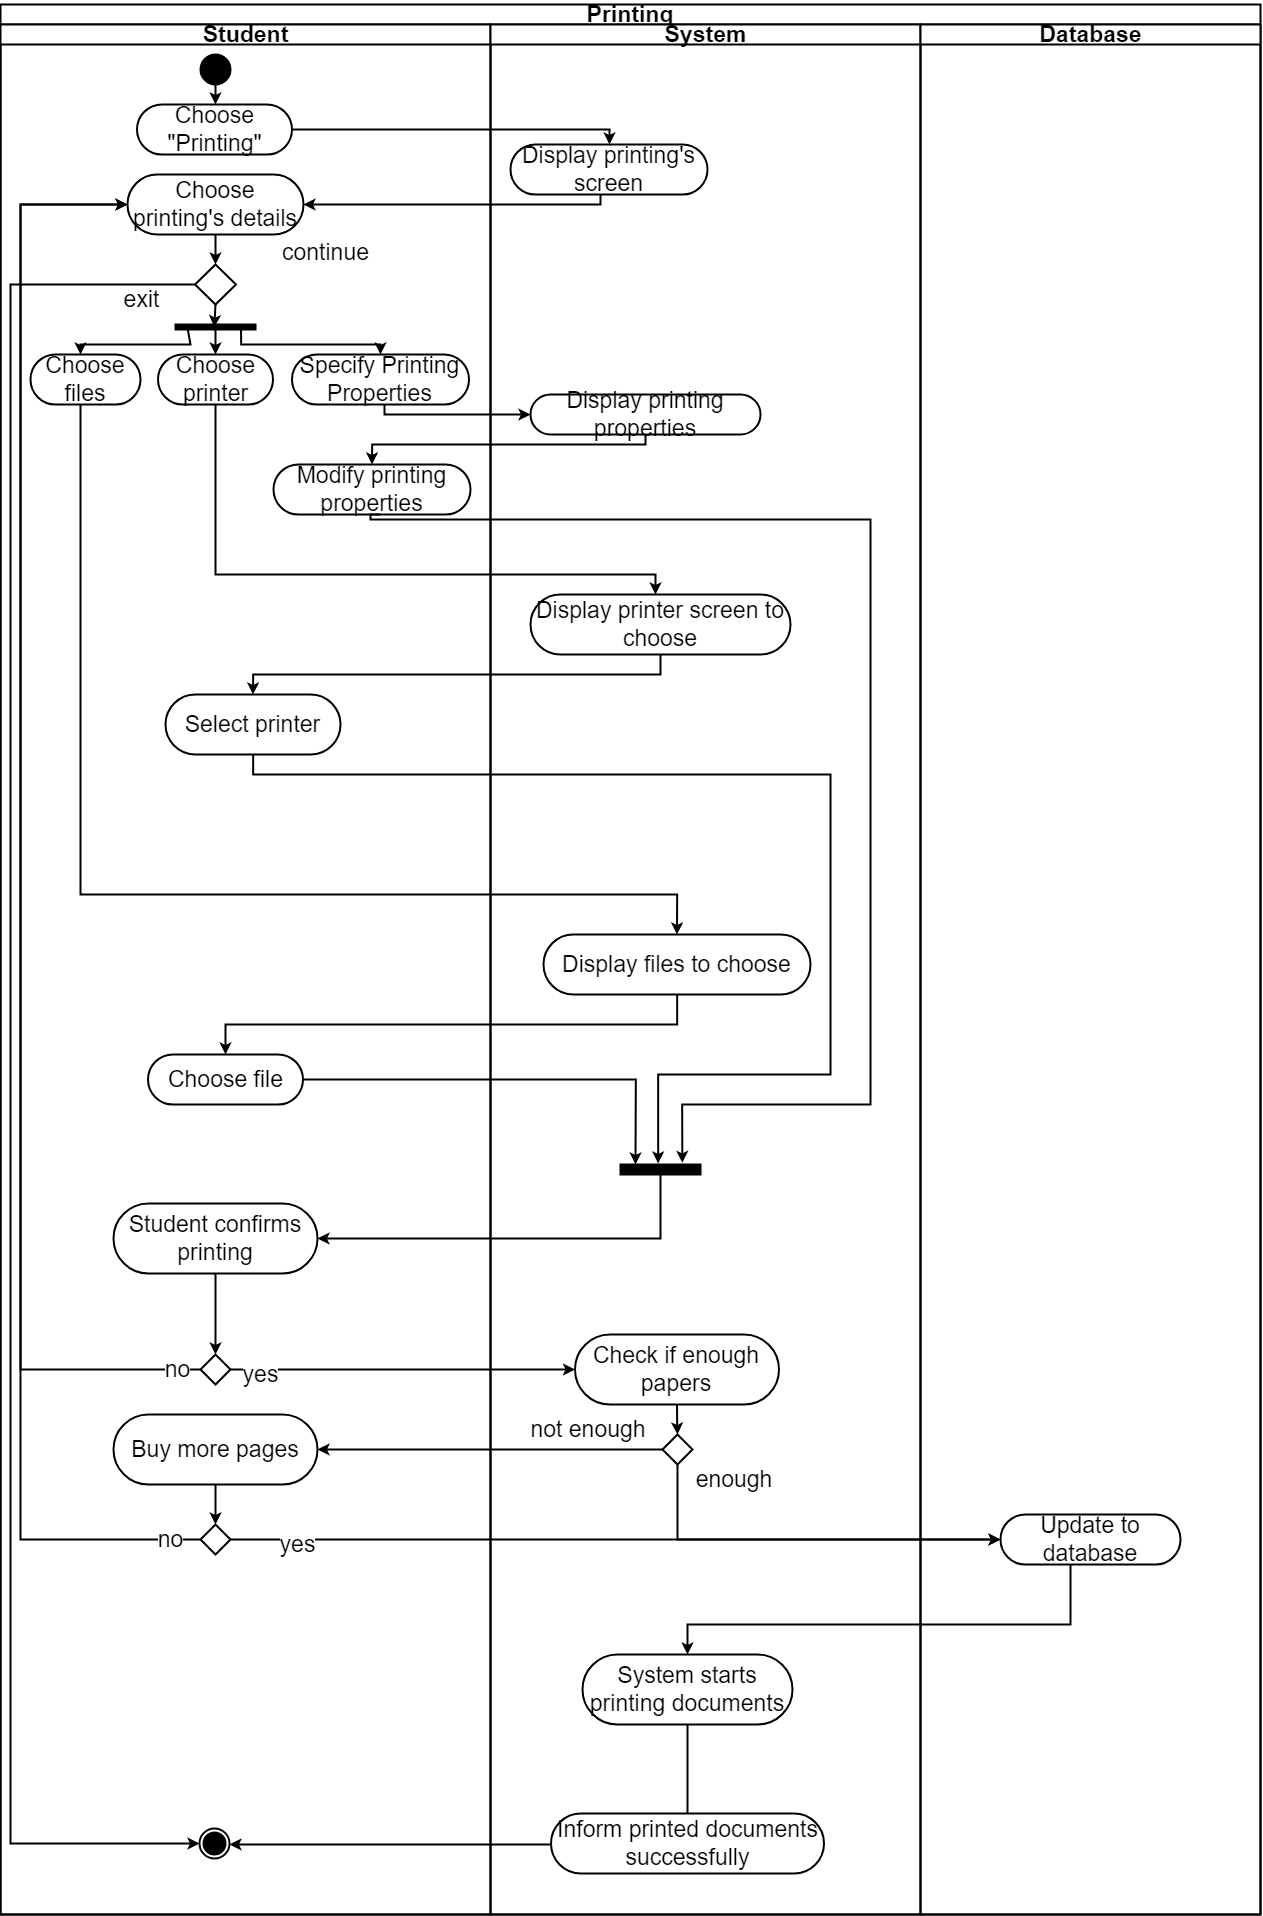
\includegraphics[width=11cm]{picture/Activiti_diagram_Print.drawio.png}
\caption{Activity diagram in}
\end{center}
\end{figure}
\newpage
\noindent \textbf{Mô tả:}\\
Người dùng truy cập vào màn hình giao diện in ấn. Hệ thống sẽ hiển thị các thao tác tùy chỉnh thông tin trước khi thực hiện in ấn. Người dùng cần chọn files từ danh sách files trong tài khoản, máy in đang hoạt động để in và chọn các thông số khi in. 

\noindent Sau khi người dùng hoàn tất chọn các thao tác trước khi in ấn, người dùng xác nhận in, hệ thống sẽ kiểm tra số trang dư của người dùng có đủ để in không.
\begin{itemize}
    \item Nếu số trang dư đủ, hệ thống sẽ tiến hành in ấn.

    \item Nếu số trang dư không đủ, hệ thống sẽ gợi ý người dùng mua thêm trang và thanh toán.
\end{itemize}

\noindent Cuối cùng, nếu đủ số trang hệ thống sẽ thông báo bắt đầu in ấn và tính toán, lưu dữ liệu vào hệ thống.


\newpage
\subsubsection{Đăng nhập}
\begin{figure}[h!]
\begin{center}
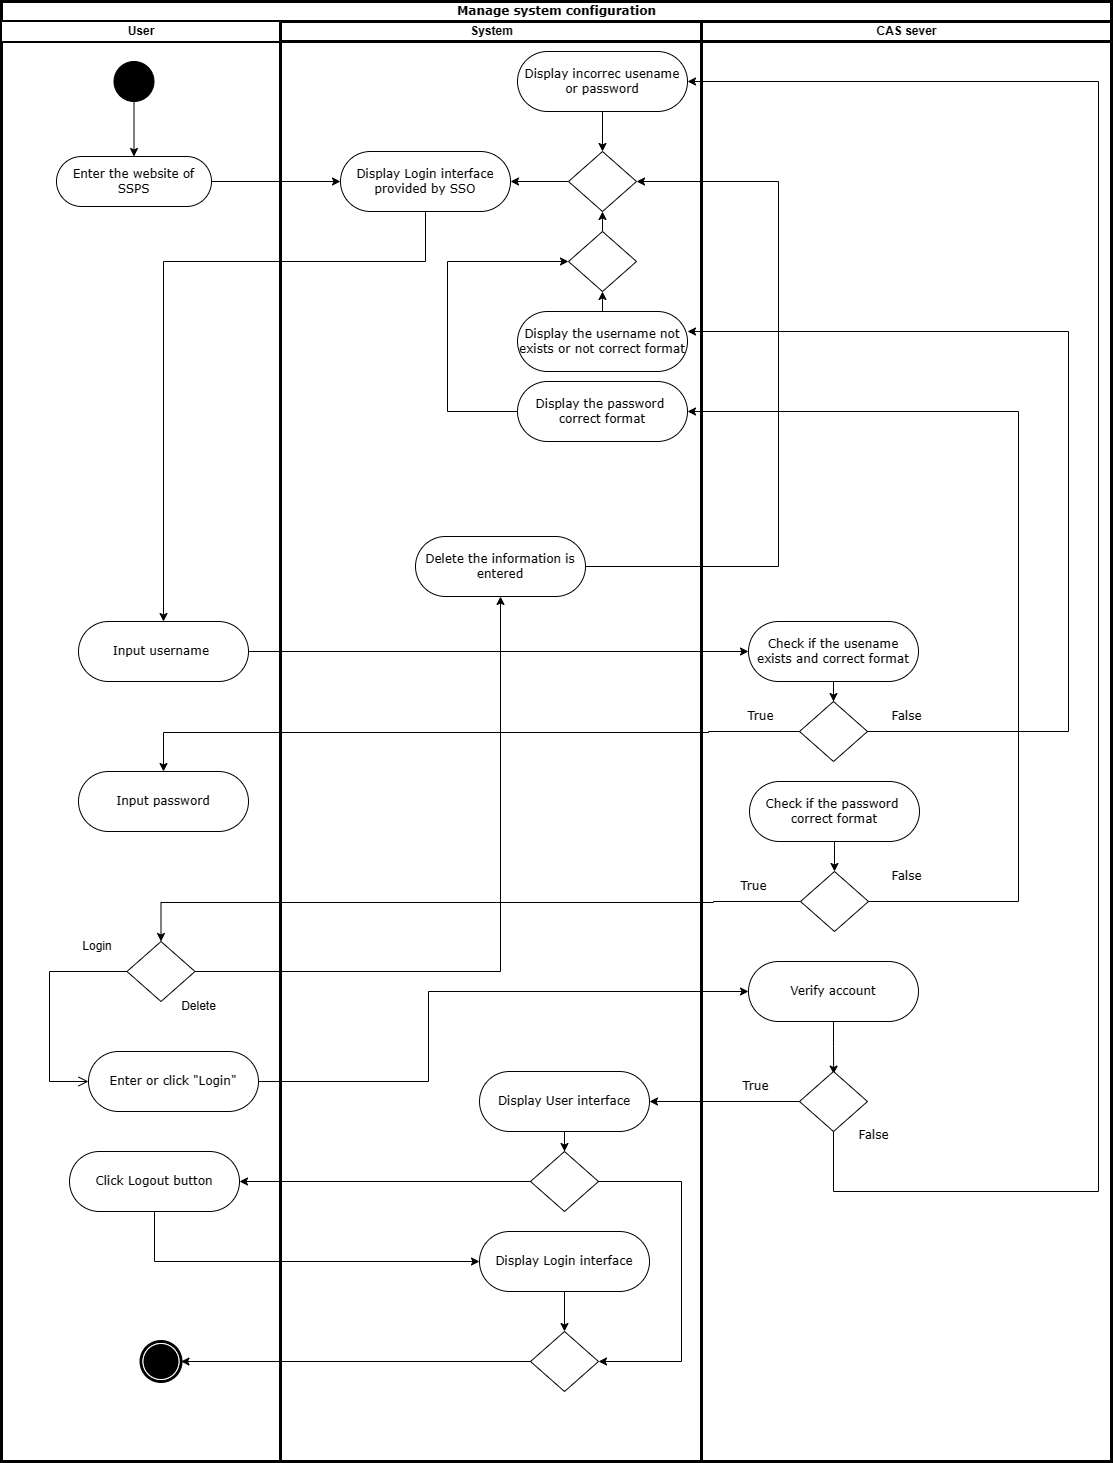
\includegraphics[width=10cm]{picture/Activiti_diagram_login-Trang-5.drawio (1).png}
\caption{Activity diagram đăng nhập}
\end{center}
\end{figure}
\newpage
\noindent \textbf{Mô tả:}\\
\noindent Activity diagram trong ảnh mô tả luồng hoạt động của quá trình đăng nhập vào hệ thống SPSS. \\
\noindent Luồng hoạt động bắt đầu khi người dùng nhập địa chỉ web của hệ thống. \\
\noindent Hệ thống sau đó hiển thị giao diện đăng nhập.

\noindent \textbf{Đầu tiên}, người dùng nhập vào tài khoản hệ thống sẽ kiểm tra xem tên người dùng đúng định dạng hoặc tồn tại không. Nếu không đúng sẽ báo ra lỗi cho người dùng thấy. \\
\noindent \textbf{Thứ hai}, người dùng nhập vào mật khẩu hệ thống sẽ kiểm tra định dạng của mật khẩu. Nếu không đúng sẽ thông báo cho người dùng vễ lồi này.\\
\noindent \textbf{Cuối cùng}, người dùng sau khi nhập xong tài khoản và mật khẩu có 2 lựa chọn là ấn nút đăng nhập hoặc xóa thông tin vừa nhập.
\begin{itemize}
    \item Nếu người dùng ấn nút “Đăng nhập” hệ thống xác minh tài khoản và hiển thị giao diện người dùng nếu tài khoản đúng. Nếu tài khoản không đúng hệ thống sẽ thông báo lỗi tài khoản nhập đã sai.
    \item Nếu người dùng ấn nút “Xóa” hệ thống sẽ xóa những thông tin vừa nhập của người dùng.
\end{itemize}

\newpage
\subsubsection{Xem số dư trang}
\begin{figure}[h!]
\begin{center}
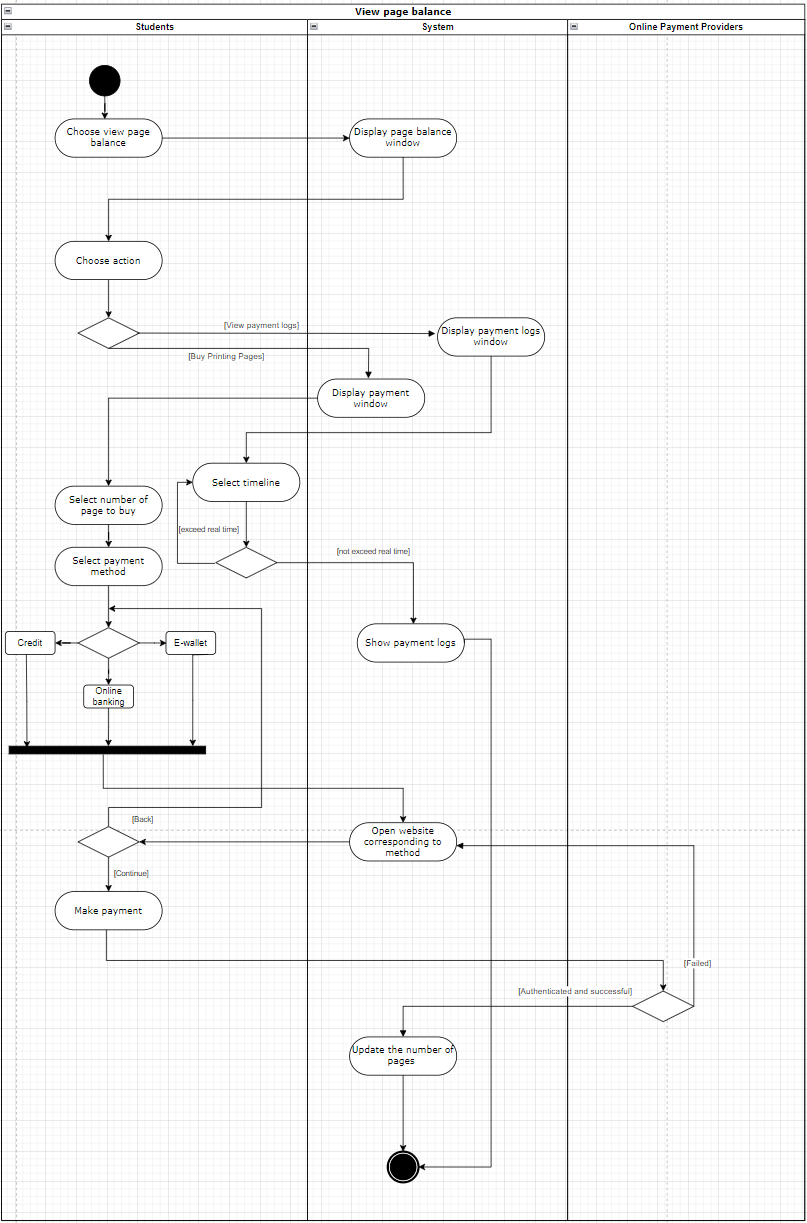
\includegraphics[width=12cm]{picture/Activity_diagram_view page blance.png}
\caption{Activity diagram xem số dư trang}
\end{center}
\end{figure}
\newpage
\noindent \textbf{Mô tả:}\\
\noindent Activity diagram cho xem số dư trang use case bắt đầu khi sinh viên bấm vào xem số trang dư. Khi đó , sinh viên sẽ nhìn thấy số trang in dư của mình của góc phải của cửa sổ giao diện.
\begin{itemize}
    \item Một là, nếu sinh viên muốn mua thêm số trang in thì chọn vào "Mua trang in", sau đó hệ thống sẽ hiển thị cửa sổ thanh toán. Sinh viên được yêu cầu chọn số trang in cần mua, sau đó chọn phương thức thanh toán (tín dụng, ngân hàng, ví điện tử). Hệ thống sẽ mở ra website tương ứng với phương thức thanh toán đã chọn. Sinh viên điền thông tin để tiến hành thanh toán. Nếu thanh toán thành công, hệ thống sẽ cập nhật số trang in trong tài khoản của sinh viên. Nếu thanh toán không thành công, sinh viên được thông báo và quay lại bước điền thông tin thanh toán.
    \item Hai là, nếu sinh viên muốn xem lịch sử giao dịch giao dịch của mình thì chọn nút "Lịch sử giao dịch", khi đó hệ thống sẽ hiển thị cửa sổ để sinh viên chọn mốc thời gian. Nếu mốc thời gian không vượt qua thời gian thực, hệ thống sẽ hiển thị thanh toán trong mốc thời gian tương ứng đó. Nếu vượt quá thời gian thực, hệ thống báo lỗi và yêu cầu sinh viên chọn lại mốc thời gian.
\end{itemize}


\newpage
\subsection{Sequence Diagram}
\subsubsection{Đăng nhập}
\begin{figure}[h!]
\begin{center}
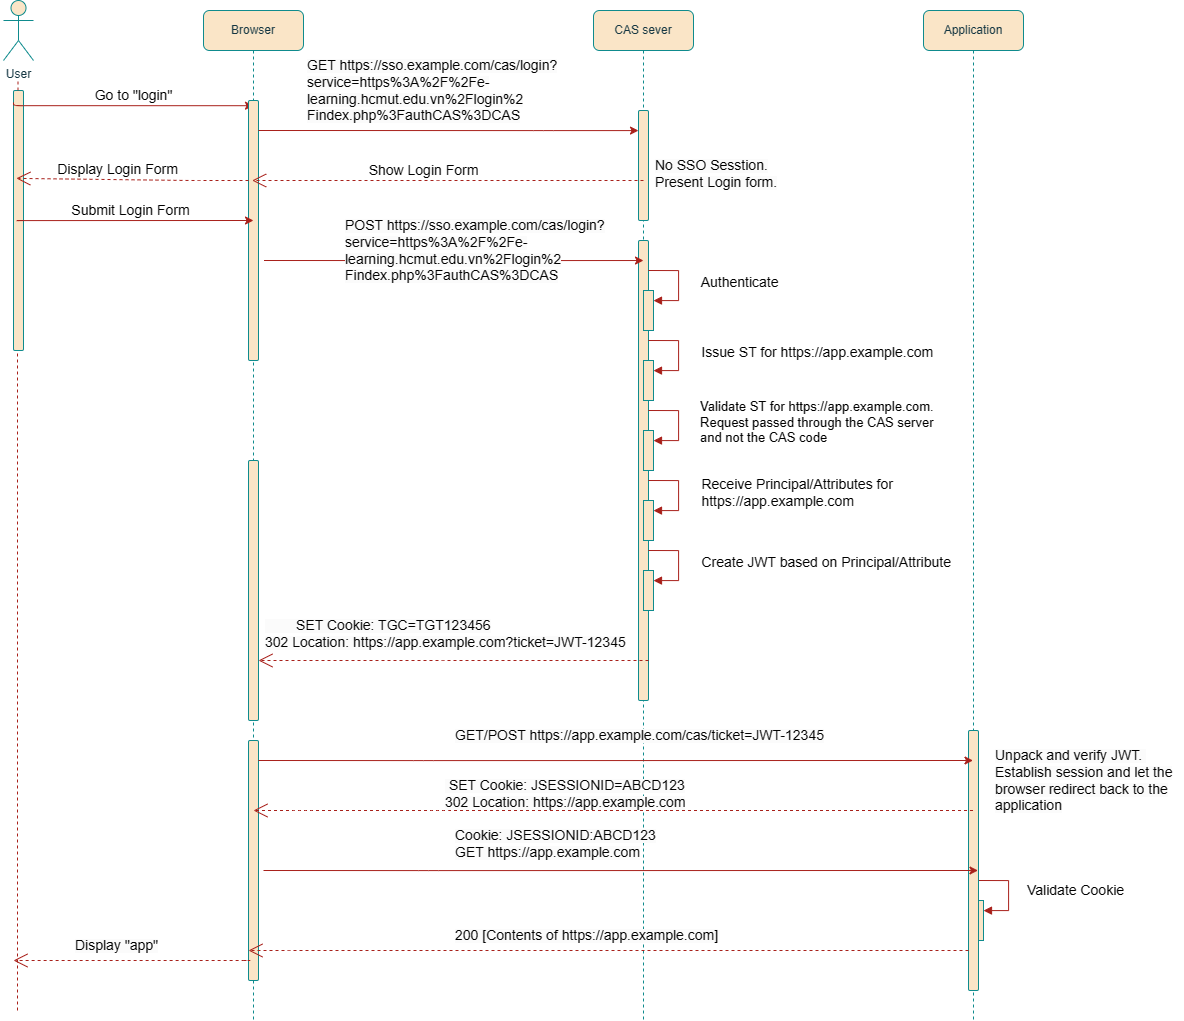
\includegraphics[width=16cm]{picture/Sequence_diagram_login-Trang-4.drawio.png}
\caption{Sequence diagram đăng nhập}
\end{center}
\end{figure}
\newpage
\noindent \textbf{Mô tả:}
\begin{itemize}
    \item Sơ đồ này mô tả quy trình xác thực người dùng cho một trang web sử dụng Single Sign-On (SSO). SSO là một phương pháp cho phép người dùng đăng nhập một lần vào nhiều ứng dụng hoặc trang web khác nhau.
    \item Quy trình bắt đầu khi người dùng truy cập vào một trang web sử dụng SSO. Trang web sẽ chuyển hướng người dùng đến máy chủ CAS, máy chủ này sẽ xác thực người dùng. 
    \item Nếu người dùng đã được xác thực, máy chủ CAS sẽ tạo một mã thông báo dịch vụ (ST). ST là một mã thông báo xác thực được sử dụng để cho phép người dùng truy cập vào các ứng dụng khác sử dụng SSO.
    \item Máy chủ CAS sẽ gửi ST đến trình duyệt của người dùng. Trình duyệt sẽ lưu ST dưới dạng cookie.
    \item Người dùng sau đó có thể truy cập vào bất kỳ ứng dụng nào sử dụng SSO mà không cần phải đăng nhập lại. Khi người dùng truy cập vào ứng dụng, ứng dụng sẽ xác thực ST trong cookie của trình duyệt. Nếu ST hợp lệ, ứng dụng sẽ cho phép người dùng truy cập.
\end{itemize}
* Chi tiết các bước:
\begin{enumerate}
    \item Người dùng truy cập vào trang web.
    \item Trang web chuyển hướng người dùng đến máy chủ CAS.
    \item Máy chủ CAS hiển thị biểu mẫu đăng nhập.
    \item Người dùng nhập thông tin đăng nhập.
    \item Máy chủ CAS xác thực người dùng.
    \item Máy chủ CAS tạo ST**.
    \item Máy chủ CAS gửi ST đến trình duyệt của người dùng.
    \item Trình duyệt lưu ST dưới dạng cookie.
    \item Người dùng truy cập vào ứng dụng.
    \item Ứng dụng xác thực ST.
    \item Ứng dụng cho phép người dùng truy cập.
\end{enumerate}
\newpage
\subsubsection{Print}
\begin{figure}[h!]
\begin{center}
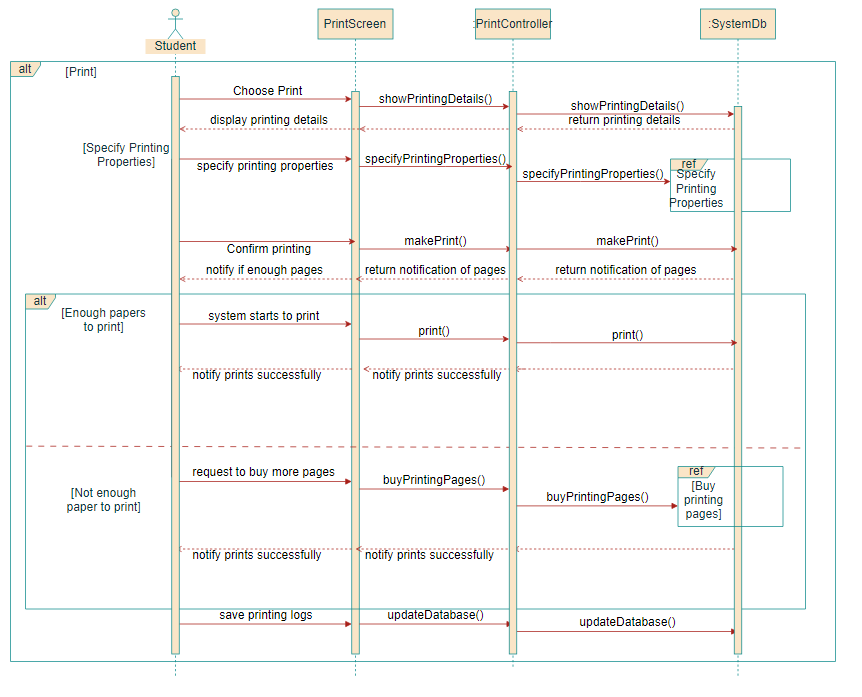
\includegraphics[width=16cm]{picture/Sequence_diagram_print.drawio.png}
\caption{Sequence diagram in}
\end{center}
\end{figure}
\clearpage
% \begin{figure}[h!]
% \begin{center}
% \includegraphics[width=16cm]{picture/Sequence_diagram_updatefiles.drawio.png}
% \caption{Sequence Diagram Update Files}
% \end{center}
% \end{figure}
% \newpage
% \begin{figure}[h!]
% \begin{center}
% \includegraphics[width=15cm]{picture/Sequence_diagram_chooseprinter.drawio.png}
% \caption{Sequence Diagram Choose Printer}
% \end{center}
% \end{figure}
\begin{figure}[h!]
\begin{center}
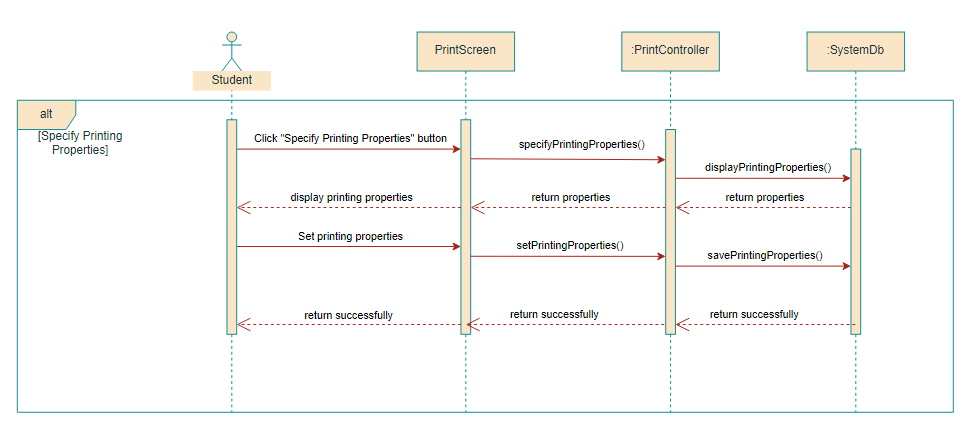
\includegraphics[width=16cm]{picture/Sequence_diagram_specifyprintingproperties.drawio.png}
\caption{Sequence diagram chỉnh sửa thông số in}
\end{center}
\end{figure}

\noindent \textbf{Mô tả:}\\
\noindent \textbf{In:}\\
\noindent - Người dùng gửi yêu cầu thực hiện in ấn thông qua giao diện In. Giao diện gửi yêu cầu về hệ thống để lấy các thông tin thao tác in ấn và hiển thị cho người dùng.\\
\noindent - Người dùng tương tác với màn hình giao diện để thực hiện các thao tác tùy chỉnh Xác định thông số in (bao gồm tùy chỉnh thông số in, chọn máy in, chọn files để in) trước khi gửi yêu cầu tiến hành in ấn.\\
\noindent - Hệ thống tiếp nhận yêu cầu thực hiện in ấn của người dùng và và kiểm tra số trang dư của người dùng.
\begin{itemize}
    \item Nếu số trang đủ, thực hiện yêu cầu in ấn của người dùng.

    \item Nếu số trang không đủ, yêu cầu người dùng mua thêm trang, nếu người dùng hoàn tất mua trang, thực hiện yêu cầu in ấn của người dùng.
\end{itemize}


\noindent \textbf{Xác định thông số in:}\\
\noindent - Người dùng gửi yêu cầu xác định các thông số tùy chỉnh in ấn, hệ thống sẽ hiển các thông tin về thông số tùy chỉnh in ấn ở màn hình giao diện các thông số in ấn.\\
\noindent - Người dùng tùy chỉnh các thông số in ấn và xác thực, hệ thống sẽ lưu lại thao tác của người dùng và thông báo xác định các thông số tùy chỉnh in ấn thành công.\\
\newpage

\subsubsection{Xem số dư trang}
\begin{figure}[h!]
\begin{center}
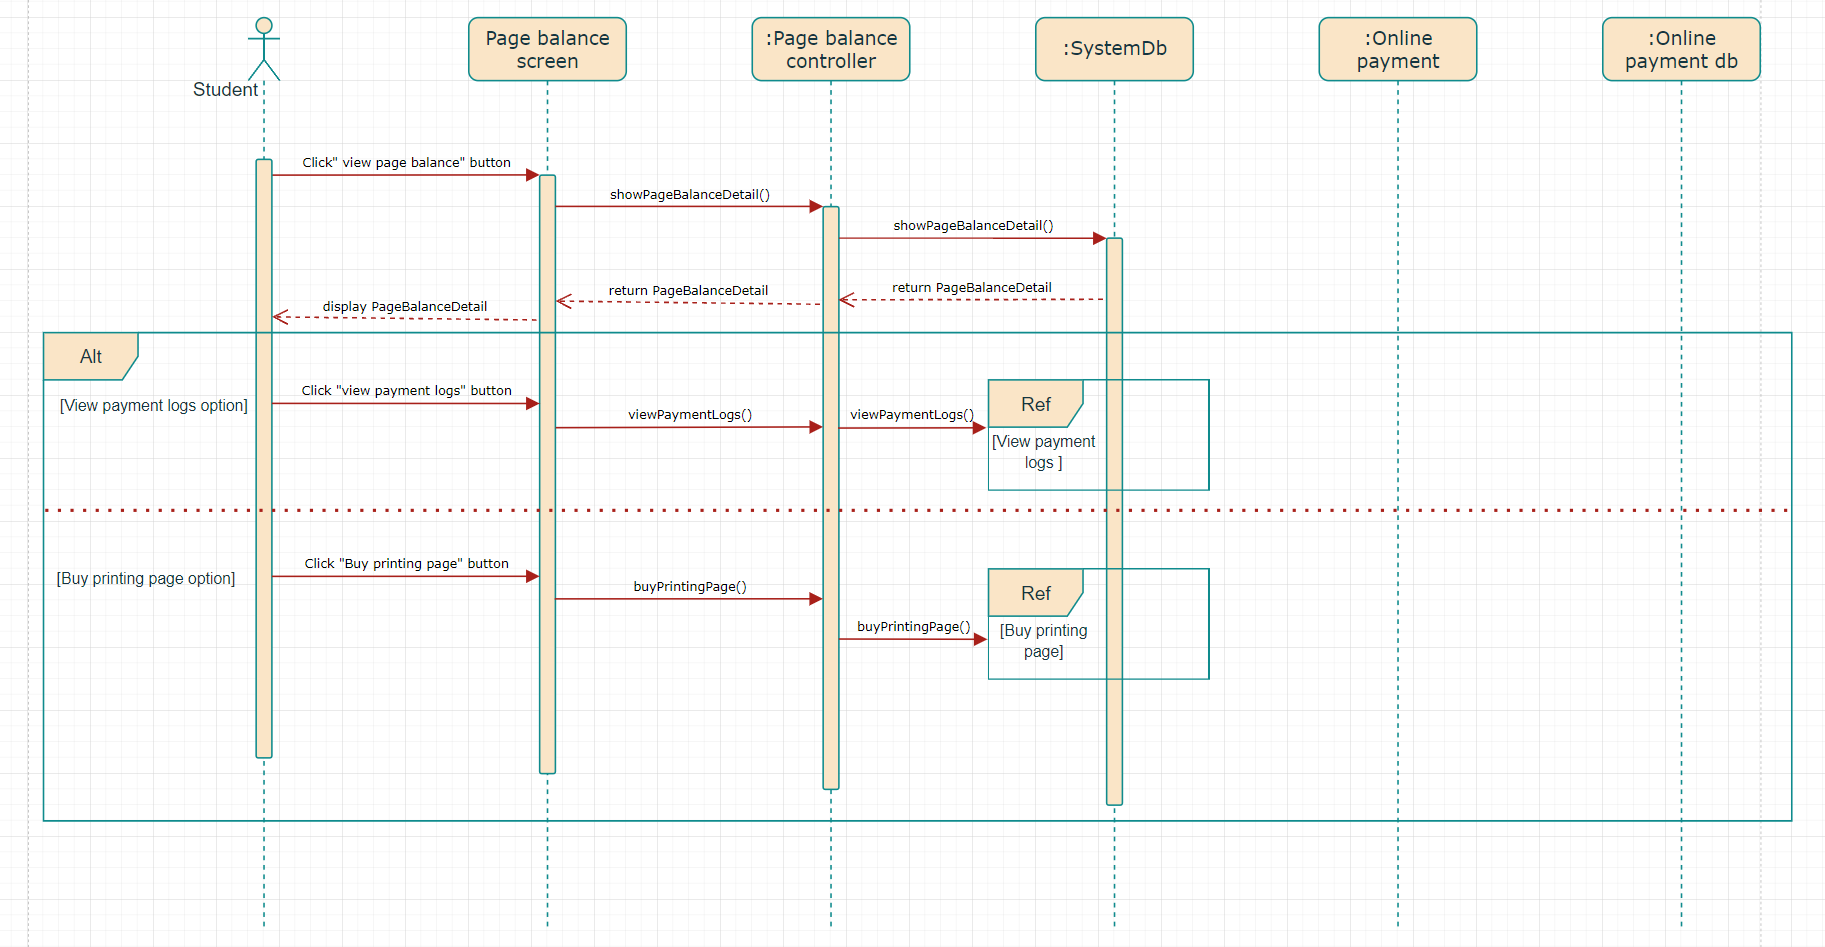
\includegraphics[width=15cm]{picture/Sequence_diagram_viewpagebalance.png}
\caption{Sequence diagram xem số trang dư}
\end{center}
\end{figure}
\begin{figure}[h!]
\begin{center}
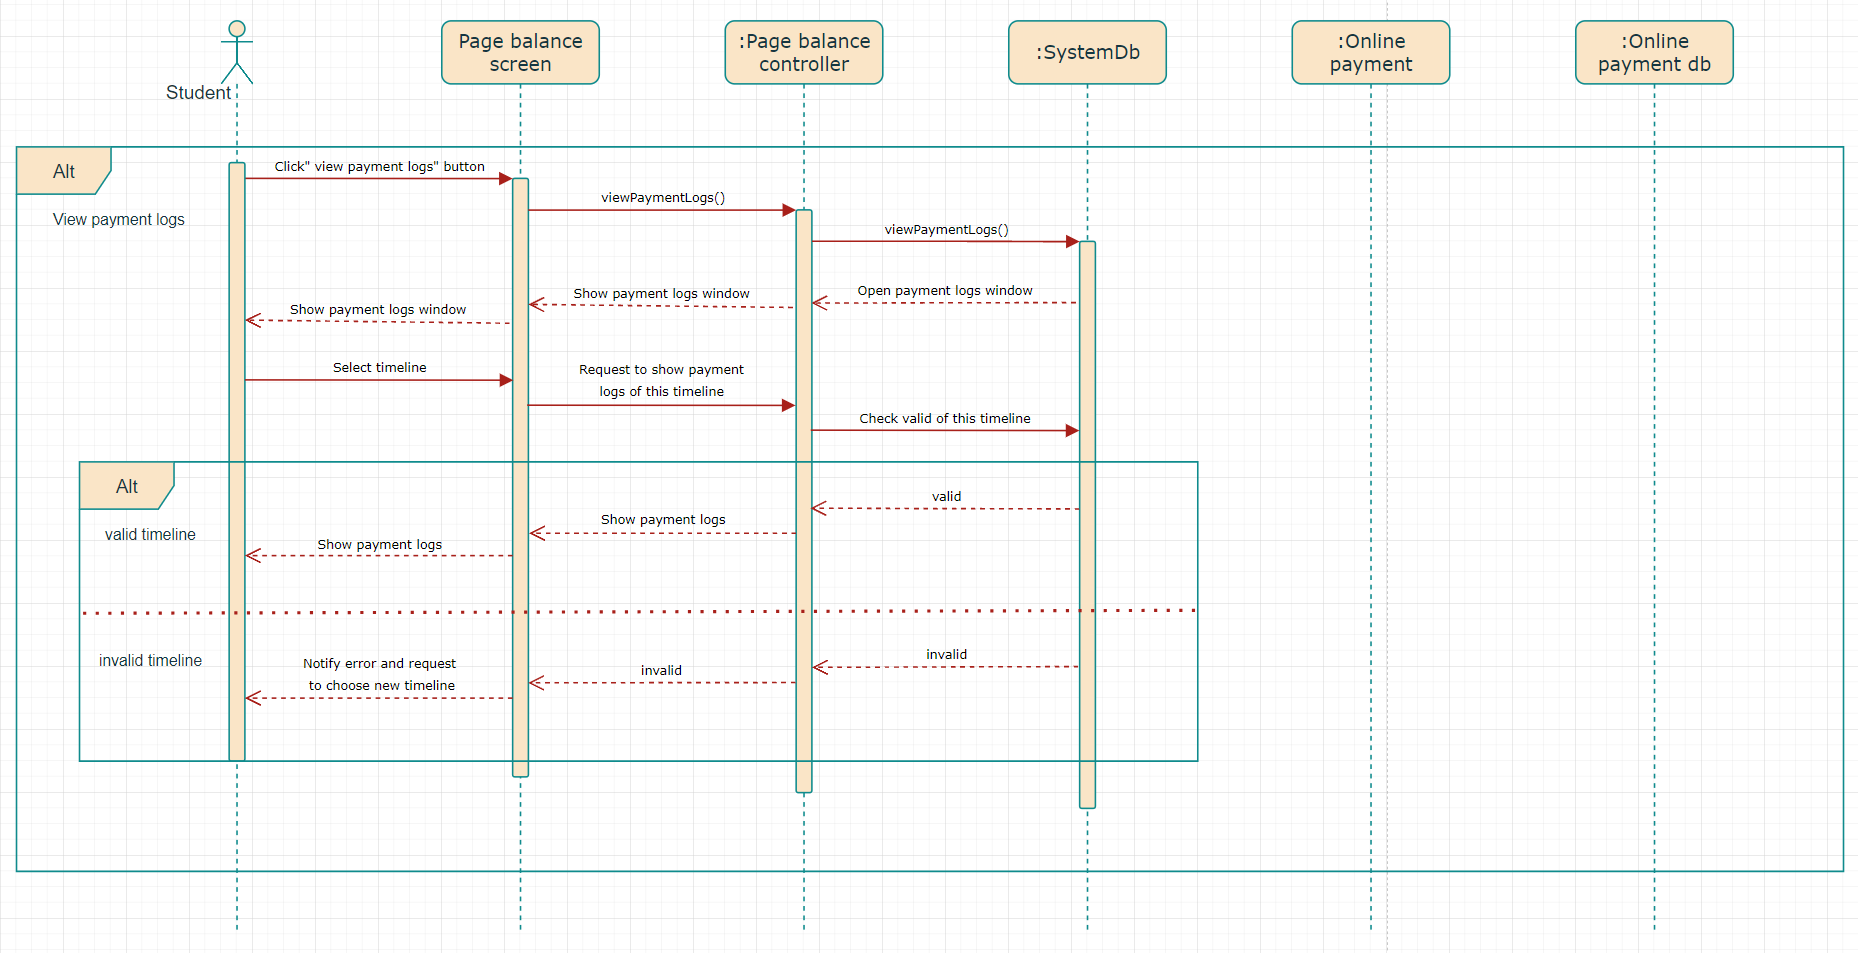
\includegraphics[width=16cm]{picture/Sequence_diagram_viewprintinglogs.png}
\caption{Sequence diagram xem lịch sử thanh toán}
\end{center}
\end{figure}
\newpage
\begin{figure}[h!]
\begin{center}
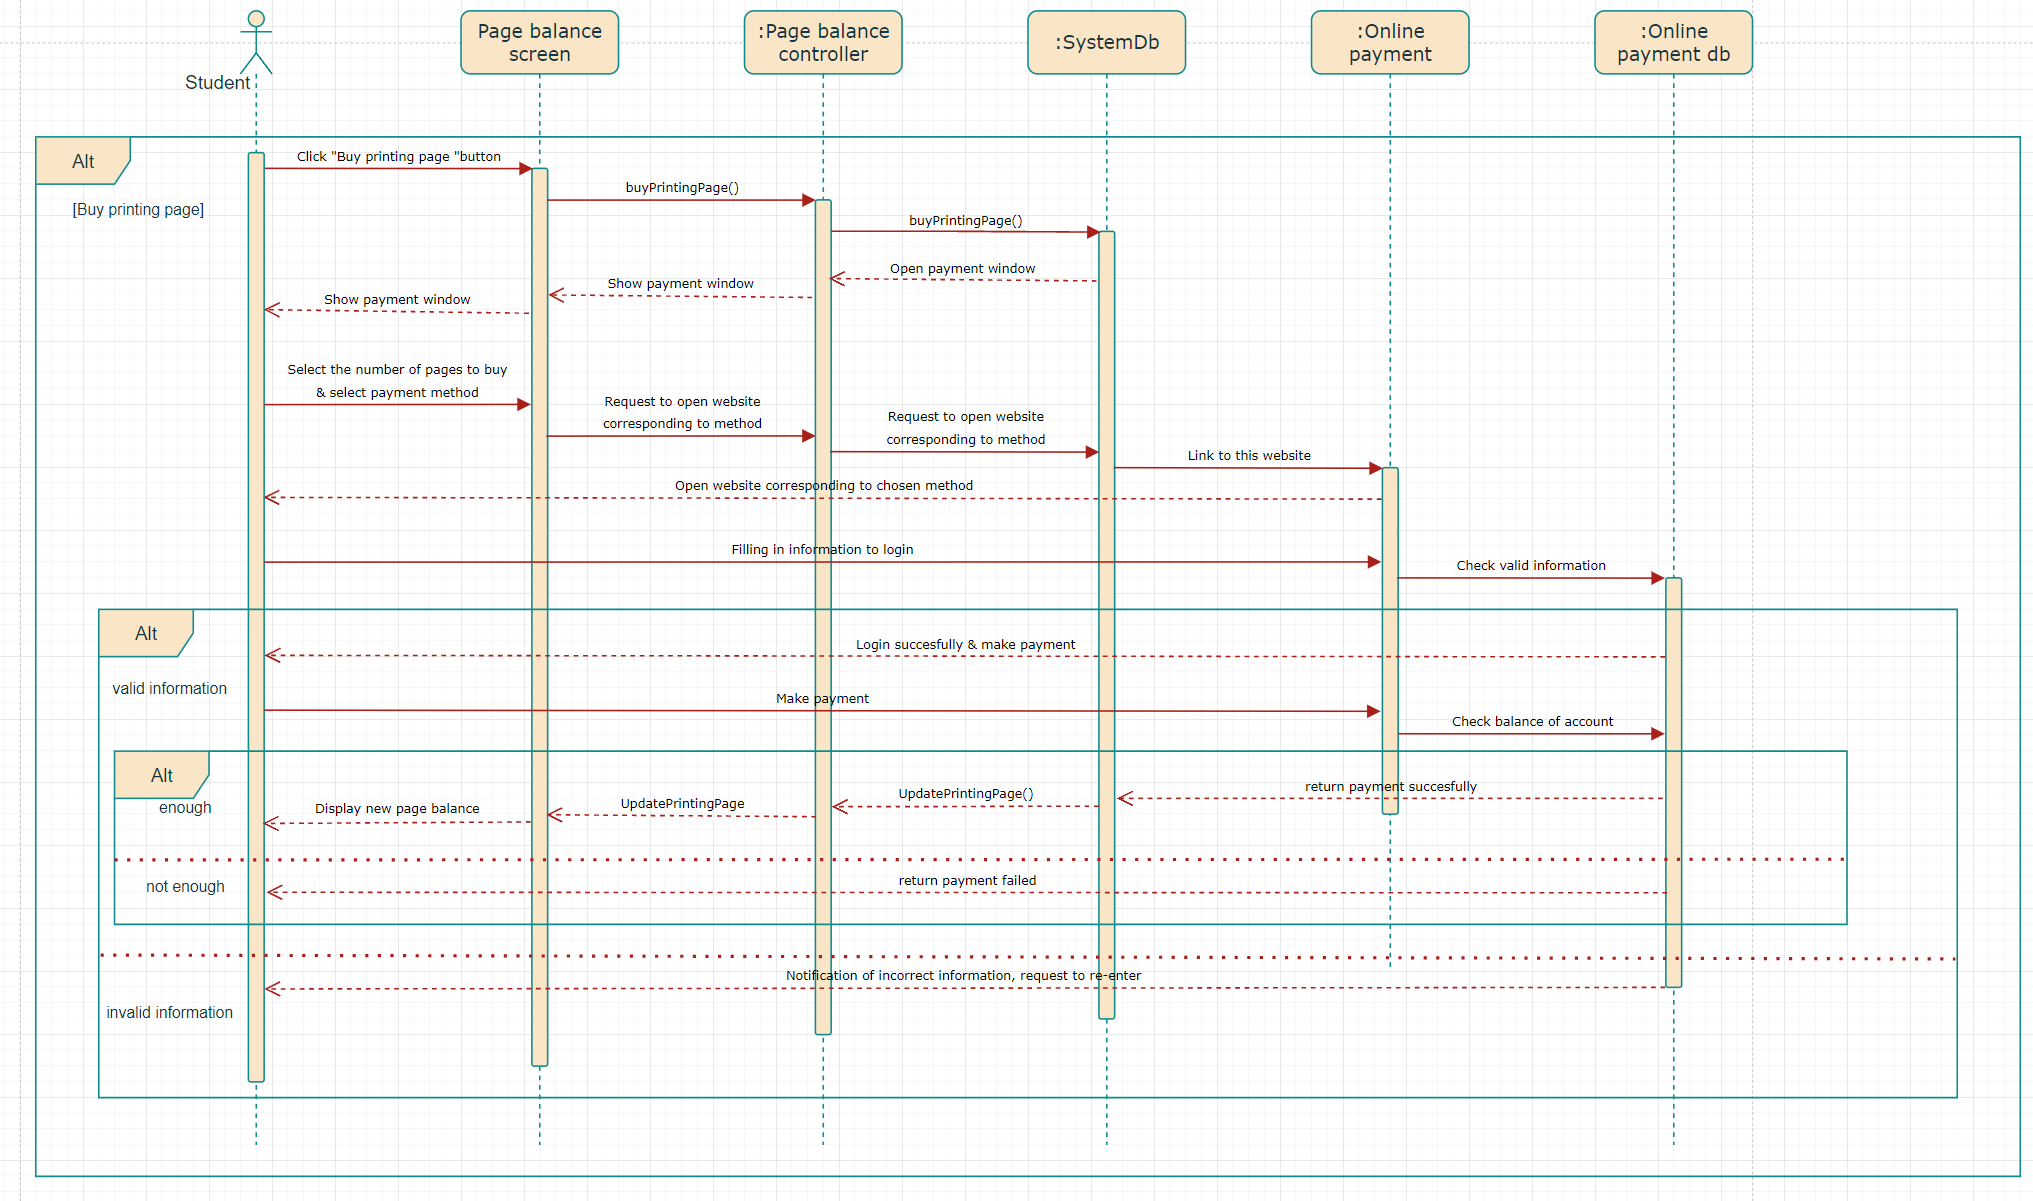
\includegraphics[width=16cm]{picture/Sequence_diagram_buyprintingpages.png}
\caption{Sequence diagram mua thêm trang}
\end{center}
\end{figure}
\noindent \textbf{Mô tả:}\\
\noindent \textbf{Xem số trang dư:}\\
\noindent - Sinh viên tạo ra một thông điệp để gửi đến hệ thống để yêu cầu xem số trang in dư. Hệ thống xử lí thông điệp, lấy số trang in dư của sinh viên và gửi trả lại kết quả cho sinh viên. Sinh viên nhận kết quả và thấy số trang in dư ở góc phải của cửa sổ giao diện.\\
\noindent \textbf{Xem lịch sử giao dịch:}\\
\noindent - Sinh viên có tùy chọn xem lịch sử giao dịch. Nếu sinh viên muốn xem lịch sử giao dịch, chọn “Lịch sử giao dịch”. Sinh viên gửi một thông điệp đến hệ thống yêu cầu xem lịch sử giao dịch. Hệ thống hiển thị cửa sổ để sinh viên chọn mốc thời gian cho lịch sử giao dịch. Sinh viên chọn mốc thời gian. Hệ thống kiểm tra mốc thời gian và hiển thị lịch sử giao dịch trong mốc thời gian đó nếu nó không vượt qua thời gian thực. Nếu mốc thời gian vượt quá thời gian thực, hệ thống báo lỗi và yêu cầu sinh viên chọn lại mốc thời gian.\\
\noindent \textbf{Mua trang in:}\\
\noindent - Sinh viên còn có tùy chọn mua trang in thêm. Nếu sinh viên quyết định mua trang in thêm, chọn “Mua trang in”. Sinh viên gửi một thông điệp đến hệ thống yêu cầu mua thêm trang in. Hệ thống sẽ mở cửa sổ thanh toán để sinh viên chọn số trang in cần mua và phương thức thanh toán. Sinh viên gửi một thông điệp tới hệ thống với thông tin đã chọn. Hệ thống kiểm tra thông tin và mở ra website tương ứng với phương thức đã lựa chọn. Sinh viên điền thông tin trên trang web. Sau đó, trang web xử lí thông tin nếu thông tin hợp lệ thì sẽ tiến hành thanh toán, nếu thông tin không hợp lệ thông báo cho sinh viên và yêu cầu nhập lại thông tin. Sau khi tiến hành thanh toán, hệ thống nhận được kết quả, nếu kết quả là thành công thì hệ thống sẽ cập nhật số trang in cho sinh viên, nếu kết quả là thất bại thì sinh viên sẽ chọn lại phương thức thanh toán.\\


\newpage
\subsection{Class Diagram}
\subsubsection{Đăng nhập}
\begin{figure}[h!]
\begin{center}
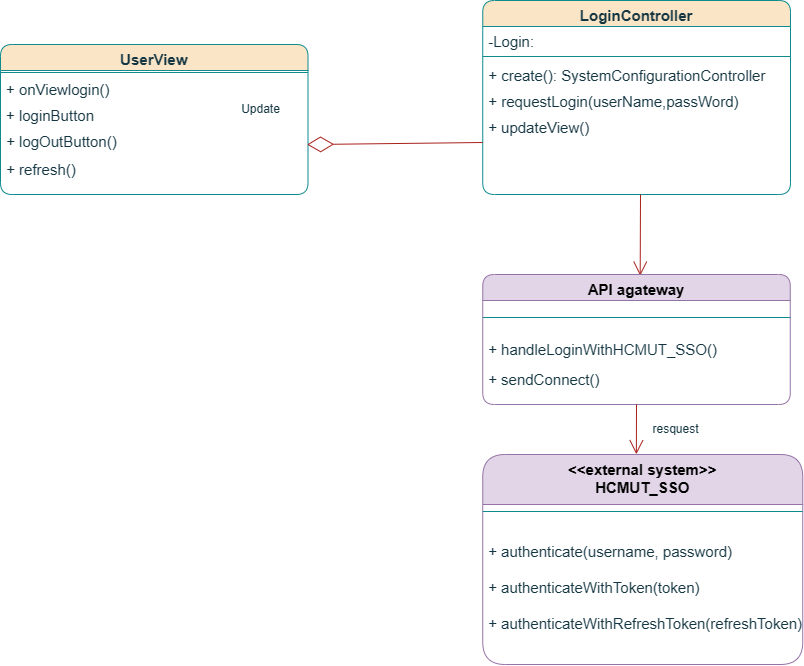
\includegraphics[width=16cm]{picture/Class_diagram_login-login.drawio (1).png}
\caption{Class diagram đăng nhập}
\end{center}
\end{figure}
\newpage
\subsubsection{In}
\begin{figure}[h!]
\begin{center}
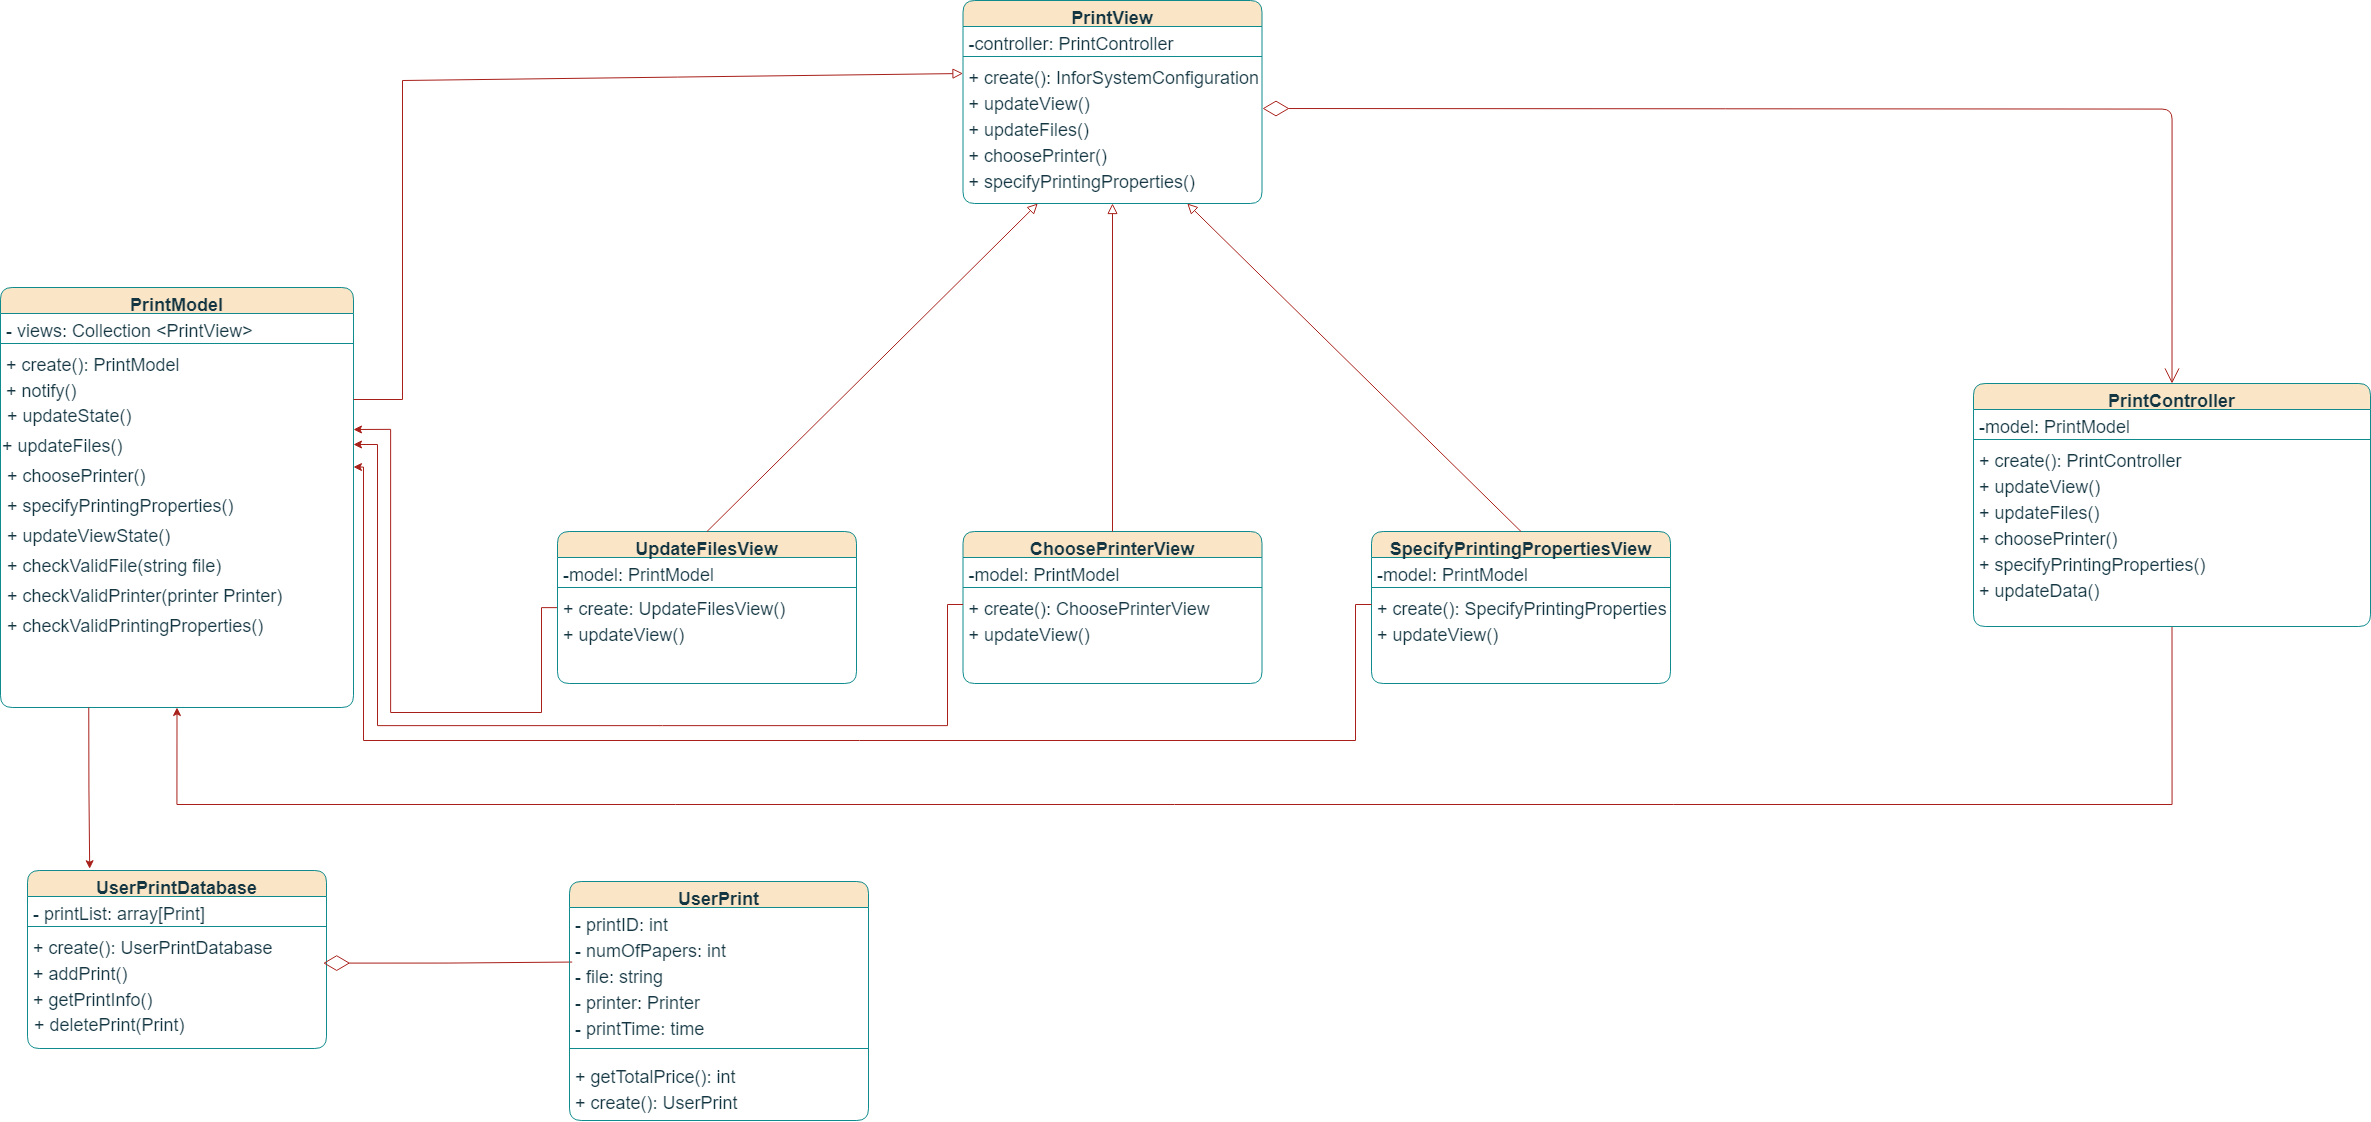
\includegraphics[width=16cm]{picture/Class_diagram_print.drawio.png}
\caption{Class diagram in}
\end{center}
\end{figure}
\newpage
\subsubsection{Xem số dư trang}
\begin{figure}[h!]
\begin{center}
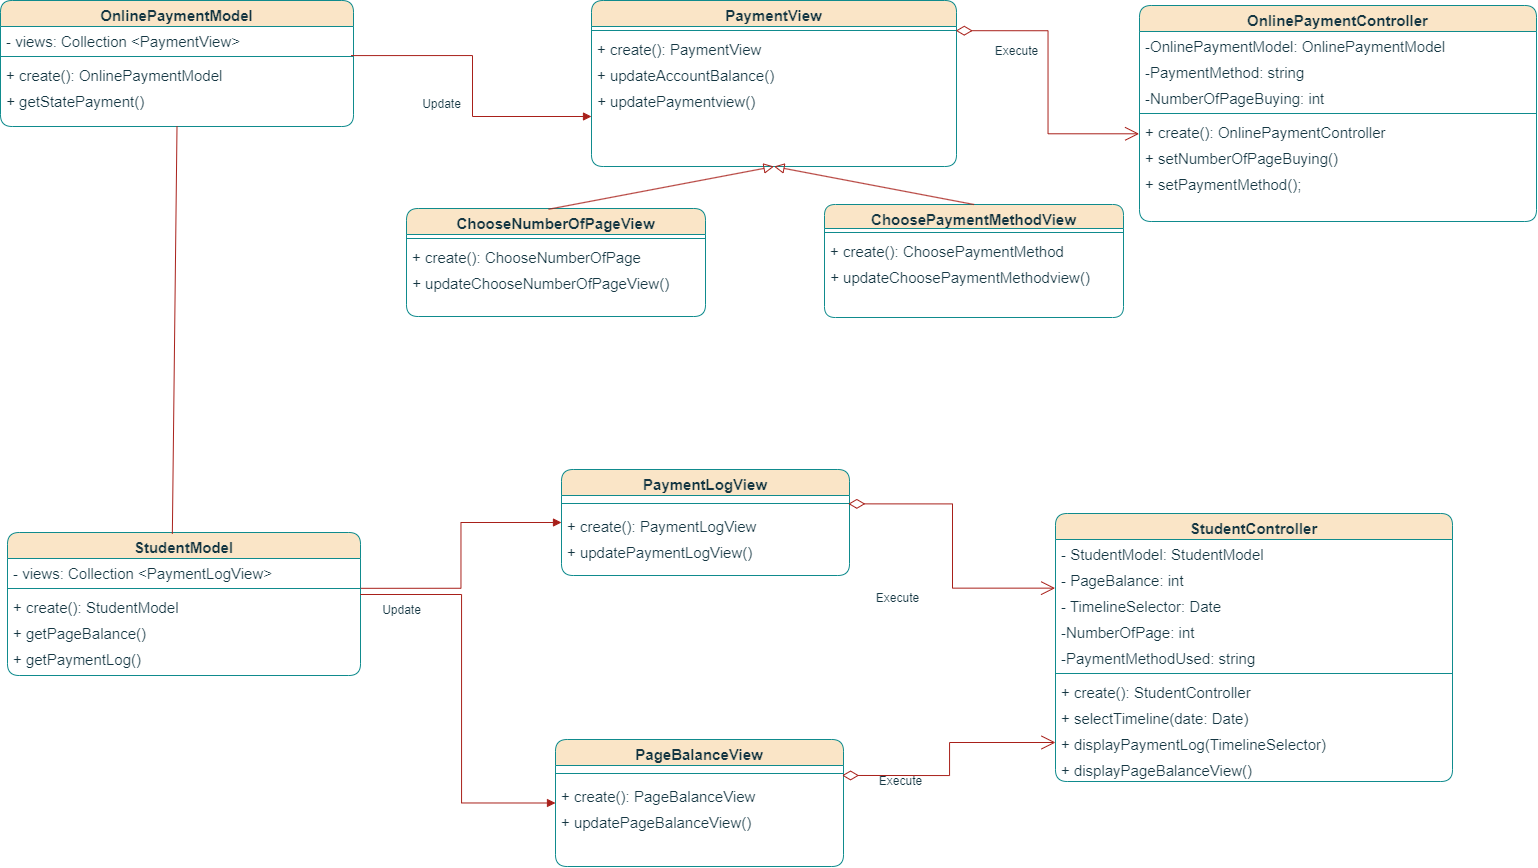
\includegraphics[width=16cm]{picture/view+buy printing page - class diagram.drawio.png}
\caption{Class diagram xem số dư trang}
\end{center}
\end{figure}
\subsection{Figma}
\noindent Nhóm thiết kế và thực hiện các yêu cầu về giao diện Figma tại: \url{https://www.figma.com/file/l05JBhuDjRbzYm0P6MwDog/Printing-service?type=design&mode=design&t=d7xrOgJ2WlRCuChN-1}
\clearpage
\section{Architecture Deisign}
\subsection{Layered Architecture}
\subsubsection{Architectural Diagram (Box-line)}
\begin{figure}[h!]
\begin{center}
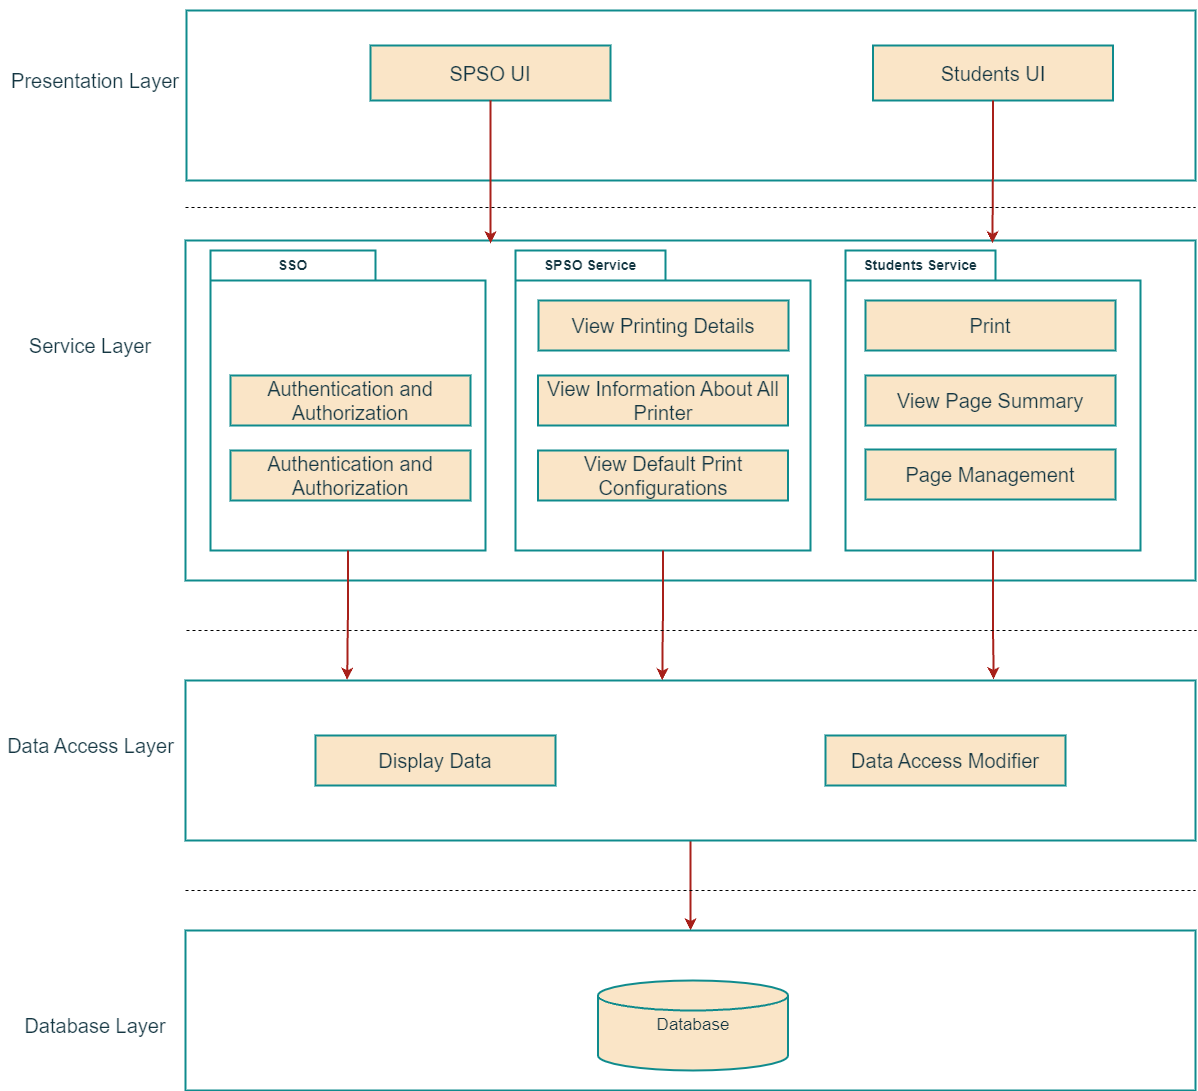
\includegraphics[width=14cm]{picture/_layered architecture.drawio.png}
\caption{Architectural diagrams của hệ thống}
\end{center}
\end{figure}
\newpage
\noindent \textbf{Chiến lược trình bày}\\
SPSS (Sinh viên Smart Printing Service) là một trang web cho sinh viên trong trường đại học có thể sử dụng các dịch vụ in ấn online. Vì vậy, giao diện người dùng nên được thiết kế đơn giản, dễ dàng sử dụng và đầy đủ chức năng.\\
\\
Nhóm sẽ triển khai “SPSO UI”, “Sinh viên UI” với HTML, CSS và ReactJS. Dựa trên thiết kế Figma ban đầu của nhóm đã hiện thực ở Task 2.4 đã cho nhóm những hình dung đầu tiên về giao diện người dùng. Tiếp theo, nhóm sẽ dựa trên thiết kế Figma tạo ra từng thành phần nhỏ dựa trên HTML, CSS, ReactJS, và sau đó sẽ tích hợp các thành phần nhỏ đó thành một trang có hiệu ứng và điều hướng.\\
\\
Lí do nhóm sử dụng HTML + CSS + ReactJS: 
\begin{itemize}
    \item Hiệu suất cao: ReactJS sử dụng Virtual Dom chỉ cập nhật các Dom thay đổi thay vì cập nhật toàn bộ.
    \item Components tái sử dụng: Tổ chức giao diện người dùng thành các components độc lập, dễ dàng tái sử dụng. Dễ dàng bảo trì và phát triển.
    \item Có cộng đồng mạnh mẽ: Có nhiều frameworks, thư viện và các mẫu thiết kế. Và khi gặp vấn đề có thể dễ dàng tìm thấy sự hỗ trợ.
    \item Tính nhất quán: CSS  \& HTML giúp đảm bảo tính nhất quán trong toàn bộ thiết kế.
\end{itemize}
\noindent \textbf{Hướng tiếp cận lưu trữ dữ liệu}

\noindent Đối với vấn đề lưu trữ dữ liệu, nhóm đã tìm ra giải pháp phù hợp là sử dụng PostgreSQL - một hệ quản trị cơ sở dữ liệu theo kiểu "object-relational" có mã nguồn mở, được phát triển bởi Đại học California, Berkeley (Hoa Kỳ) vào 1996. PostgreSQL cho phép người dùng tự do sử dụng, chỉnh sửa và phân bổ theo nhiều hình thức khác nhau.\\

\noindent Lý do nhóm quyết định lựa chọn sử dụng PostgreSQL bởi vì những tính năng quan trọng và cần thiết cho dự án mà nó sở hữu:
\begin{itemize}
    \item Đa dạng về kiểu dữ liệu: PostgreSQL cung cấp nhiều kiểu dữ liệu như nguyên hàm (các nguyên số, boolean, số, chuỗi), cấu trúc (UUID, Range, Array, Date/time), hình học, tùy chỉnh và document.
    \item Tính toàn vẹn dữ liệu: Dữ liệu trong PostgreSQL được đảm bảo tính toàn vẹn nhờ vào các khóa như Primary Keys, Foreign Keys, UNIQUE, NOT NULL, Khóa hàm số/ Explicit Locks, Khóa khuyến nghị/ Advisory Locks,...
    \item Tính bảo mật: PostgreSQL hỗ trợ xây dựng hàng rào bảo mật, xác thực mạnh mẽ
    \item Khả năng mở rộng: Người dùng có thể thực hiện mở rộng hệ thống qua các hình thức lưu trữ, kết nối cơ sở dữ liệu (CSDL), ngôn ngữ thủ tục, PostGIS, tính năng kết nối CSDL hoặc luồng khác với giao diện SQL chuẩn,…
\end{itemize}
\noindent Ngoài ra, PostgreSQL cung cấp một cách sử dụng đơn giản, dễ hiểu nhưng đem lại hiệu quả cao trong việc vận hành cơ sở dữ liệu.\\

\noindent Đối với việc lưu trữ và quan trị cơ sở dữ liệu
trong yêu cầu bài tập lớn lần này, nhóm sẽ dùng PostgreSQL để lưu trữ và xử lý các thông tin, loại dữ liệu như sau:
\begin{itemize}
    \item Thông tin đăng nhập của người dùng: tài khoản và mật khẩu (Vì nguồn dữ liệu về tài khoản, mật khẩu MyBK của trường Đại học Bách Khoa TP HCM được bảo mật, nhóm không thể xin phép sử dụng được nên quyết định tạo mới và quản lý một hệ thống tài khoản, mật khẩu tương tự như MyBK)

    \item Thông tin lưu trữ về việc in ấn, máy in.
\end{itemize}

\noindent \textbf{Quản lí API}\\
Về mặt kỹ thuật, \textbf{API} là viết tắt của Giao diện lập trình ứng dụng (Application Programming Interface), một trung gian phần mềm cho phép hai ứng dụng giao tiếp với nhau, có thể sử dụng cho web-based system, operating system, database system, computer hardware, or software library. \\\\
Ở dạng đơn giản nhất, API là giao diện cho phép một ứng dụng giao tiếp với ứng dụng khác thông qua các lệnh đơn giản và cách các lệnh này được gửi và định dạng mà dữ liệu được truy xuất thông qua API có thể khác với \textbf{API SOAP} hoặc \textbf{REST(Representational State Transfer)}.\\\\
\textbf{RESTful API} là một tiêu chuẩn dùng trong việc thiết kế các API cho các ứng dụng web để quản lý các resource. \textbf{RESTful} là một trong những kiểu thiết kế API được sử dụng phổ biến ngày nay để cho các ứng dụng (web, mobile…) khác nhau giao tiếp với nhau.\\\\
Chức năng quan trọng nhất của REST là quy định cách sử dụng các HTTP method (như \textbf{GET, POST, PUT, DELETE…}) và cách định dạng các URL cho ứng dụng web để quản các resource. RESTful không quy định logic code ứng dụng và không giới hạn bởi ngôn ngữ lập trình ứng dụng, bất kỳ ngôn ngữ hoặc framework nào cũng có thể sử dụng để thiết kế một \textbf{RESTful API}.\\
\begin{figure}[h!]
\begin{center}
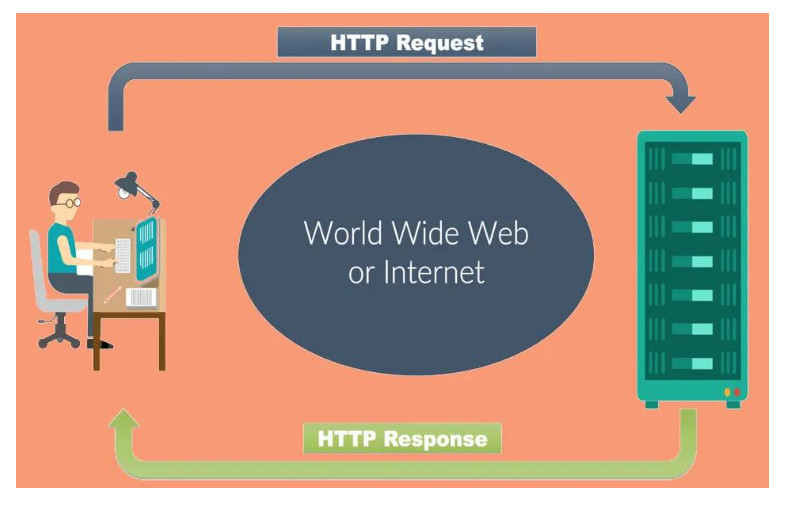
\includegraphics[width=12cm]{picture/anh 1.jpg}
\end{center}
\end{figure}
\clearpage
\noindent \textbf{HTTP – Hypertext Transfer Protocol }là giao thức được thiết kế và hoạt động theo kiểu client-server. Giao tiếp giữa client và server dựa vào một cặp là HTTP Request- HTTP Response. Khi một client đưa ra request, server trả lời bằng các response ngay sau đó. Và API được xây dựng trên chính 2 thành phần: Request và Response. Cấu trúc của mỗi thành phần :\\
\textbf{Request}\\
Một request đúng chuẩn cần có 3 thứ:
\begin{itemize}
    \item Request Line: gồm URL và method.
    \item Headers
    \item Body
\end{itemize}
\begin{figure}[h!]
\begin{center}
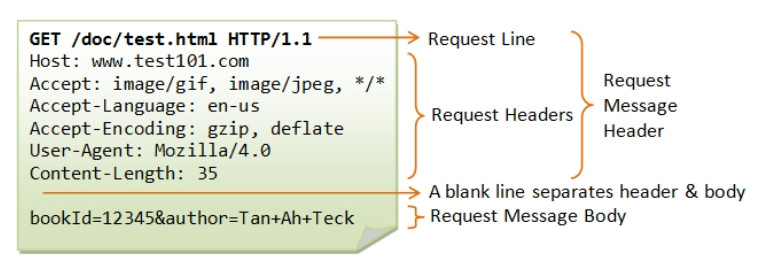
\includegraphics[width=14cm]{picture/anh 2.jpg}
\end{center}
\end{figure}
Chi tiết như sau :
\begin{itemize}
    \item \textbf{URL} là 1 địa chỉ duy nhất cho 1 thứ (dùng danh từ), có thể là web page, image hoặc video. API mở rộng cái ý tưởng gốc của URL cho những thứ khác, ví dụ customers, products. Và như thế client dễ dàng cho server biết cái nó muốn là cái gì, những cái này còn được gọi chung là “resources” – nguồn lực.
    \item \textbf{Method} là hành động client muốn tác động lên “resources”, và nó thường là động từ. 
\end{itemize}
\begin{figure}[h!]
\begin{center}
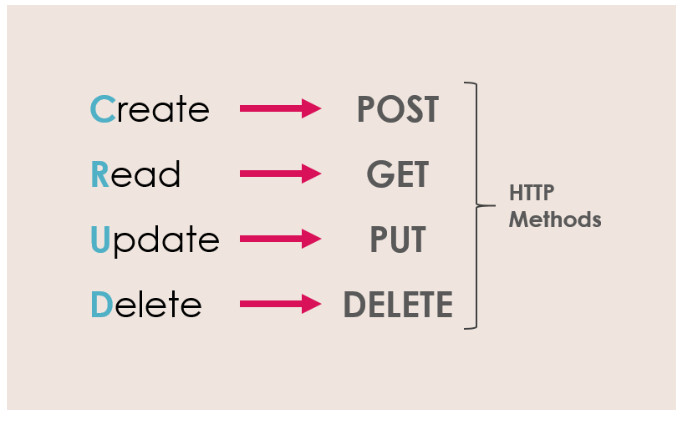
\includegraphics[width=14cm]{picture/anh 3.jpg}
\end{center}
\end{figure}
 Có 4 loại method hay được dùng và các ví dụ về các method của API quản lý máy in:\\
– \textbf{GET}: Yêu cầu server đưa lại resource. Ví dụ lấy thông tin chi tiết của một máy in.\\
– \textbf{POST}: Yêu cầu server cho tạo ra 1 resource mới. Ví dụ: tạo một máy in mới.\\
– \textbf{PUT}: Yêu cầu server cho sửa / thêm vào resource đã có trên hệ thống. Ví dụ:
cập nhật thông tin của một máy in.\\
– \textbf{DELETE}: Yêu cầu server cho xóa 1 resource. Ví dụ : Xóa một máy in.\\
• \textbf{Headers}: nơi chứa các thông tin cần thiết của 1 request nhưng end-Người dùngs không biết có sự tồn tại của nó. Ví dụ: độ dài của request body, thời gian gửi request, loại thiết bị đang sử dụng, loại định dạng response mà client có đọc được.\\
• \textbf{Body}: nơi chứa thông tin mà client sẽ điền. Giả sử bạn đặt 1 cái bánh pizza, thì thông tin ở phần body sẽ là: Loại bánh pizza, kích cỡ, số lượng đặt.
Respond\\
Sau khi nhận được request từ phía client, server sẽ xử lý cái request đó và gửi ngược lại cho client 1 response. Cấu trúc của 1 response tương đối giống phần request những Status code sẽ thay thế cho URL và Method. \\Tóm lại, nó có cầu trúc 3 phần:
\begin{itemize}
    \item Status line
    \item Headers
    \item Body
\end{itemize}
\begin{figure}[h!]
\begin{center}
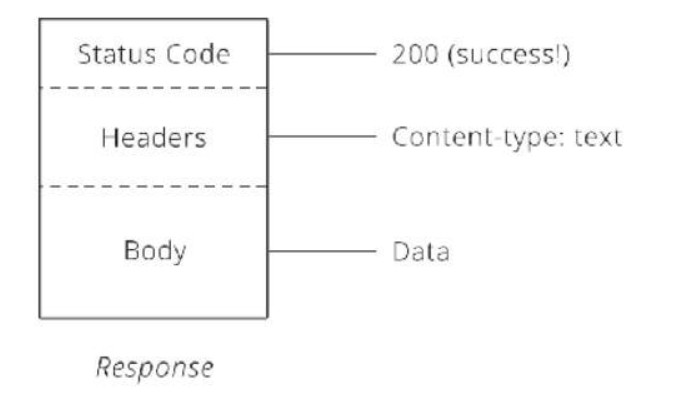
\includegraphics[width=14cm]{picture/anh 4.jpg}
\end{center}
\end{figure}
\textbf{Ví dụ:}\\
HTTP/1.1 200 OK
Date: Mon, 31 Oct 2023 10:30:00 GMT
Content-Type: text/html
Content-Length: 1024\\
Các API chính\\
Hệ thống API của chúng tôi cung cấp các API sau:
\begin{itemize}
    \item API quản lý tài khoản người dùng: API này cho phép người dùng đăng nhập, đăng xuất và quản lý mật khẩu.
    \item API quản lý máy in: API này cho phép người dùng xem danh sách máy in, trạng thái máy in và các thông tin khác liên quan đến máy in.
    \item API quản lý tài liệu: API này cho phép người dùng tải lên, tải xuống, xóa và quản lý các tài liệu của mình.
    \item API in tài liệu: API này cho phép người dùng in tài liệu của mình trên các máy in.
    \item API quản lý lịch sử in ấn: API này cho phép người dùng xem lịch sử in ấn của mình.
    \item API quản lý báo cáo: API này cho phép người dùng xem các báo cáo về việc sử dụng dịch vụ in ấn.
\end{itemize}
\textbf{}\textbf{Quản lý APIs}\\
Là quá trình tạo, xuất bản và quản lý các kết nối API trong nền tảng đa “đám mây” và trong một doanh nghiệp. Không chỉ là nơi để kết nối các API lại với nhau, việc quản lý API tạo ra một nền tảng thống nhất và có thể mở rộng mà cho phép các doanh nghiệp chia sẻ và đưa ra những cấu hình API của họ trong khi vẫn kiểm soát truy cập, thu thập và phân tích thống kê sử dụng, và thực hiện các chính sách bảo mật liên quan.\\
Để quản lý API cho hệ thống in ấn thông minh dành cho sinh viên tại HCMUT, nhóm sử dụng các công nghệ sau:
\begin{itemize}
    \item \textbf{React}: React là một thư viện JavaScript mã nguồn mở để xây dựng giao diện người dùng (UI). React được chọn vì nó có khả năng phát triển UI nhanh chóng và hiệu quả, đồng thời dễ dàng bảo trì và mở rộng.
    \item \textbf{PHP}: PHP là một ngôn ngữ lập trình mã nguồn mở được sử dụng để phát triển các ứng dụng web. PHP được chọn vì nó có tốc độ xử lý nhanh, dễ học và sử dụng, đồng thời có một cộng đồng lớn các nhà phát triển hỗ trợ.
    \item \textbf{REST API}: REST API là một kiến trúc thiết kế API dựa trên các phương thức HTTP và các tài nguyên được biểu diễn dưới dạng JSON. REST API được chọn vì nó đơn giản, linh hoạt và dễ dàng sử dụng.
    \item \textbf{PostgreSQL}: PostgreSQL là một hệ quản trị cơ sở dữ liệu mã nguồn mở. MySQL được chọn vì nó có độ tin cậy cao, các tính năng mạnh, ổn định và hiệu suất cao.
\end{itemize}


\newpage
\subsubsection{Deployment Diagram}
\begin{figure}[h!]
\begin{center}
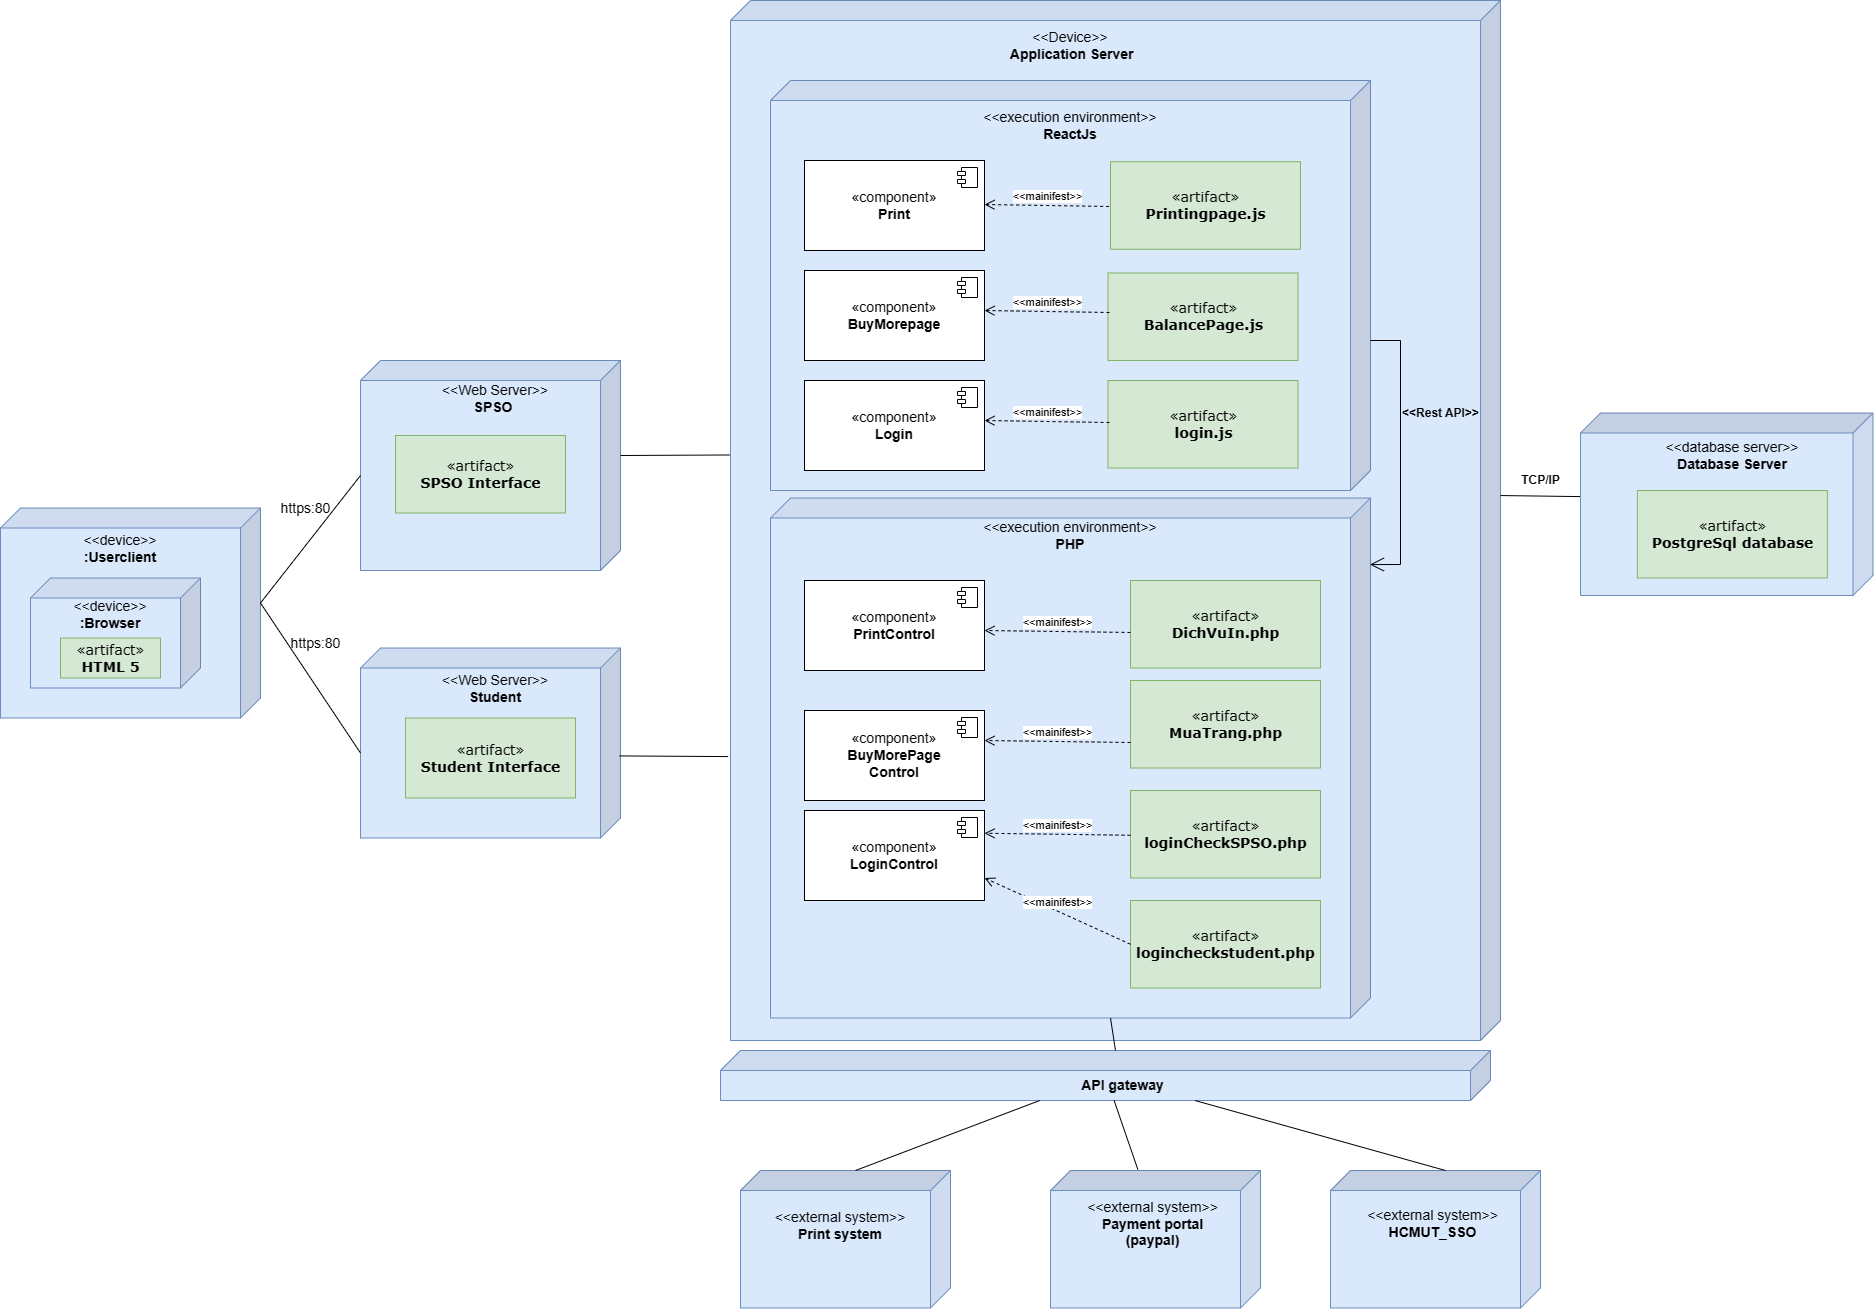
\includegraphics[width=16cm]{picture/deployment_diagram-Trang-2.drawio (1).png}
\caption{Deployment diagram của hệ thống}
\end{center}
\end{figure}
Máy chủ ứng dụng (Application Server) là nơi lưu trữ và chạy các dịch vụ ứng dụng của hệ thống. Trong trường hợp này, máy chủ ứng dụng bao gồm các dịch vụ sau:
\begin{itemize}
    \item Cổng đăng nhập(login) được hiện thực trong reactjs là file login.js và trong php là file logincheckspso.php và logincheckstudent.php
    \item In ấn (Print) được hiện thực trong reactjs là file Printingpage.js và trong php là file DichVuIn.php
    \item Mua thêm trang (BuyMorePage)  được hiện thực trong reactjs là file BalancePage.js và trong php là file MuaTrang.php
\end{itemize}
Máy chủ web (Web Server) là nơi lưu trữ các trang web và xử lý các yêu cầu từ người dùng. Trong trường hợp này, máy chủ web:
\begin{itemize}
    \item Giao diện dành cho student.
    \item Giao diện dành cho spso.
\end{itemize}

Cơ sở dữ liệu (Database) là nơi lưu trữ dữ liệu của hệ thống. Trong trường hợp này, cơ sở dữ liệu là một cơ sở dữ liệu PostgreSQL.\\
Hệ thống in ấn (Printing System) là nơi in các tài liệu của hệ thống.

\textbf{Các hệ thống bên ngoài }
\begin{itemize}
    \item Hệ thống thanh toán (Payment System) là nơi xử lý các giao dịch thanh toán của hệ thống. Trong trường hợp này, hệ thống thanh toán là một cổng thanh toán PayPal.
    \item Hệ thống quản lý tài khoản của user: HCMUT\_SSO.
    \item Hệ thống in: bao gồm việc xác nhận giao dịch in cho sinh viên.
\end{itemize}
\subsection{Component Diagram}
\subsubsection{Component diagram cho module đăng nhập }
\begin{figure}[h!]
\begin{center}
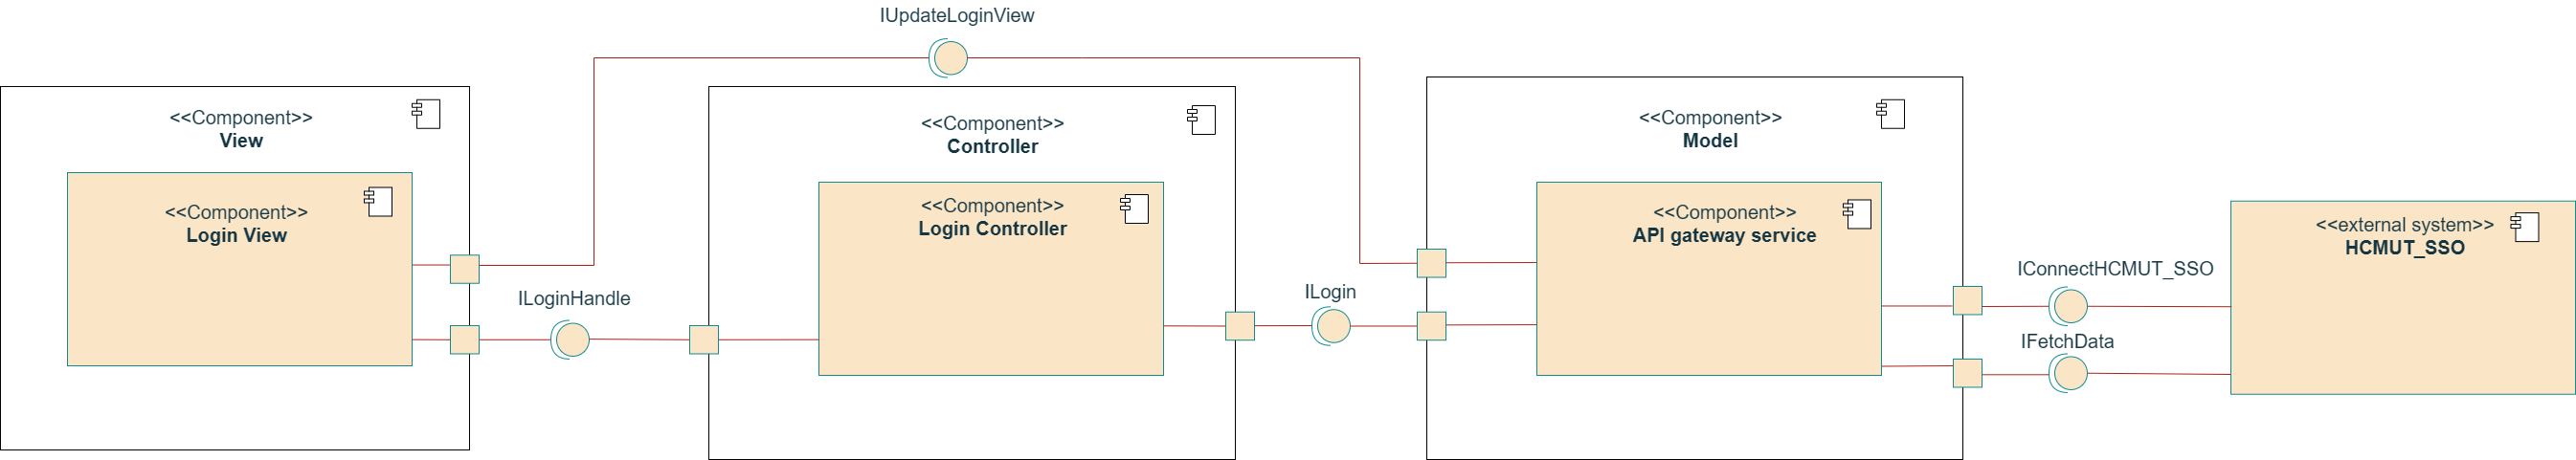
\includegraphics[width=16cm]{picture/Login_component-Trang-3.drawio.png}
\caption{Component diagram cho module đăng nhập}
\end{center}
\end{figure}

\noindent \textbf{Mô tả}

\noindent \textbf{a. Component}

\textbf{Login View:} Là giao diện người dùng cho ứng dụng. Nó bao gồm các trường nhập liệu để người dùng nhập tên người dùng và mật khẩu của họ.

\textbf{Login Controller:} Là lớp điều khiển cho ứng dụng. Nó chịu trách nhiệm xử lý dữ liệu từ Login View và xác thực người dùng.

 \textbf{API Gateway Service Component:} là một trung tâm điều phối thông minh, giúp kết nối các ứng dụng, dịch vụ và tài nguyên khác nhau một cách hiệu quả, an toàn và có thể mở rộng.
 
\textbf{HCMUT\_SSO:} là nơi quản lý tài khoản user và thực hiện các thao tác xác thực thông tin đăng nhập cho user.
\newpage
\noindent \textbf{b. Interface}
%%%%
\begin{table}[h!]
\centering
\begin{tabular}{|M{4cm}|p{5cm}|p{6.5cm}|}
\hline
\textbf{Tên interface} & \textbf{Chức năng} & \textbf{Các phương thức} \\
\hline
ILoginHandle &Quản lý các chức năng liên quan đến đăng nhập  & Các phương thức chính \\
\hline
IUpdateLoginView & Cập nhật giao diện đăng nhập & login(userName,pwd) \\
\hline
ILogin & Thực hiện quá trình đăng nhập & requestLogin(userName,pwd) \\
\hline
IconnectHCMUT\_SSO & Kết nối đến hệ thống đăng nhập Single Sign-On (SSO) của HCMUT & sendConnect()\\
\hline
IFetchData\_SSO & Gửi yêu cầu truy xuất dữ liệu từ hệ thống SSO của HCMUT & sendRequestVerifyLogin(username,pwd)\\
\hline
\end{tabular}
\end{table}


%%%%%
\begin{comment}
\begin{figure}[h!]
\begin{center}
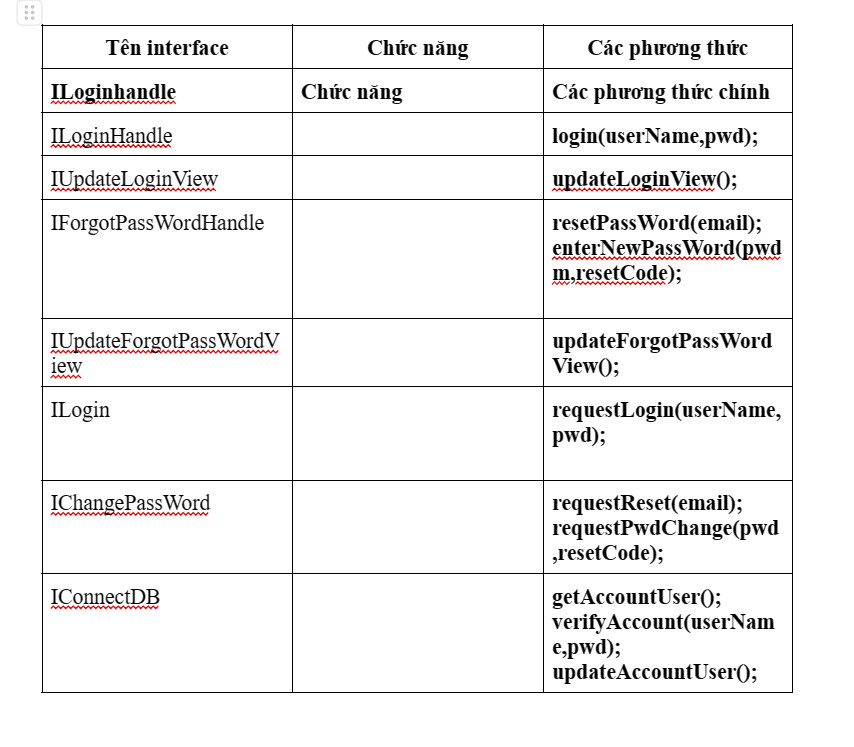
\includegraphics[width=16cm]{picture/mô tả function for interface login 3.2.jpg}
\caption{Chức năng các interface của module đăng nhập}
\end{center}
\end{figure}
\clearpage
\subsubsection{Component Diagram for  Print action in module Print }
\begin{figure}[h!]
\begin{center}
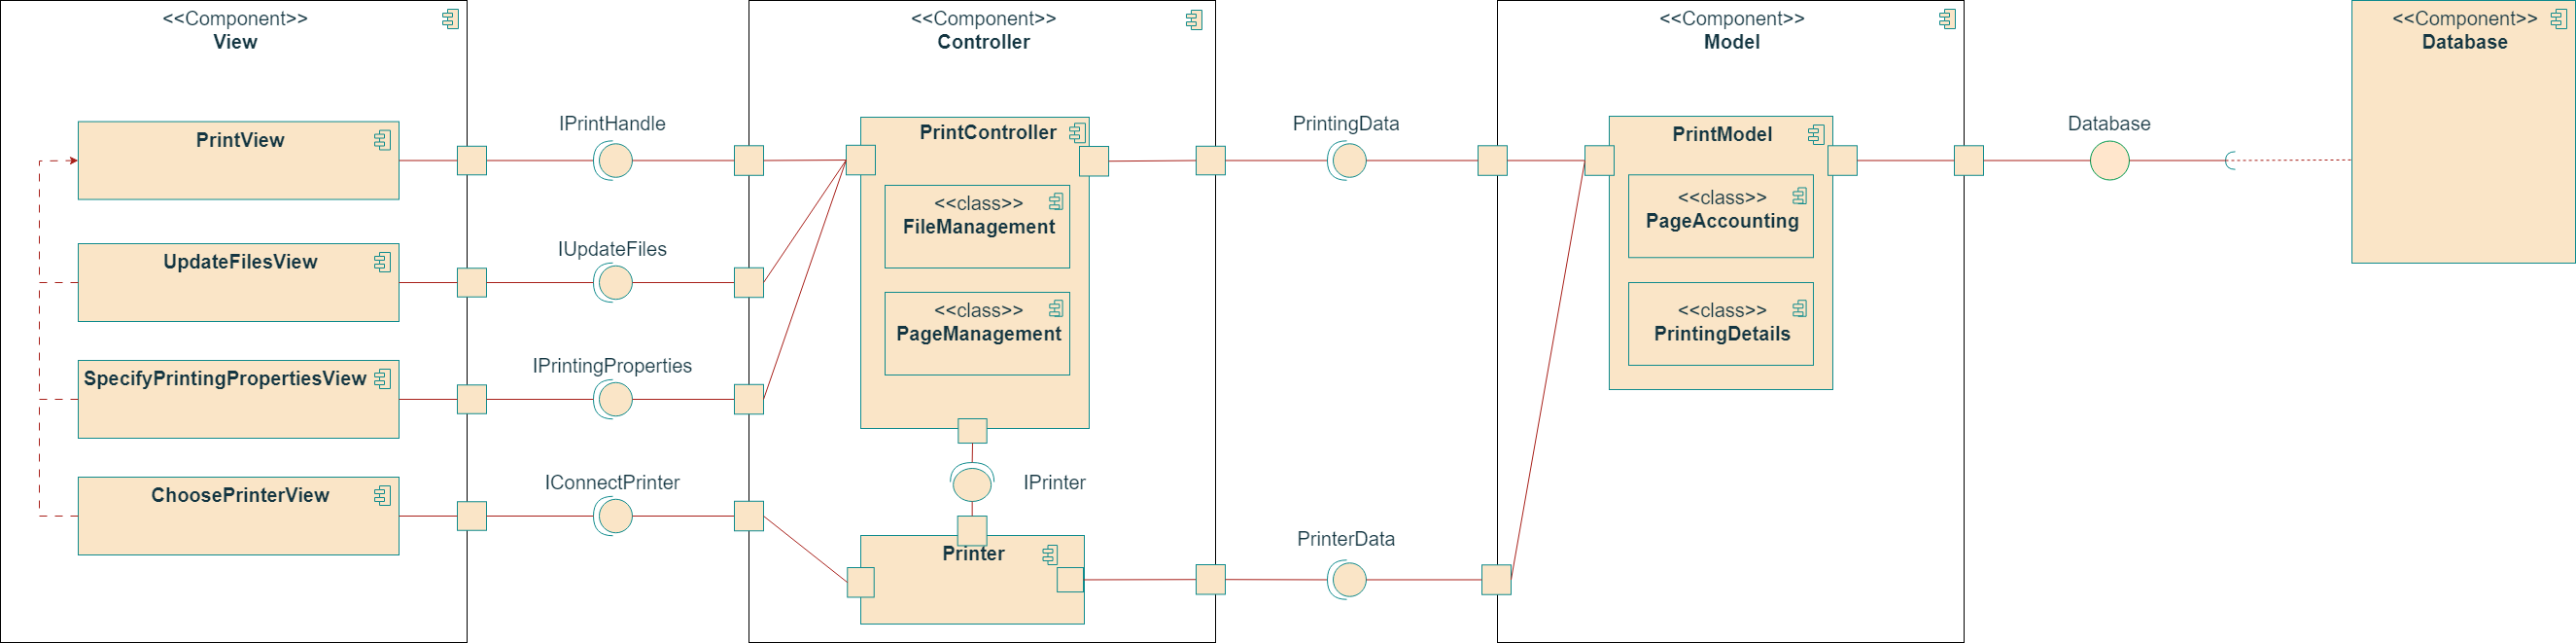
\includegraphics[width=16cm]{picture/3.2.Component_Print.drawio.png}
\caption{Mô tả hàm cho các interface trong component print}
\end{center}
\end{figure}
\end{comment}
\subsubsection{Component Diagram của chức năng In trong module In}
\begin{figure}[h!]
\begin{center}
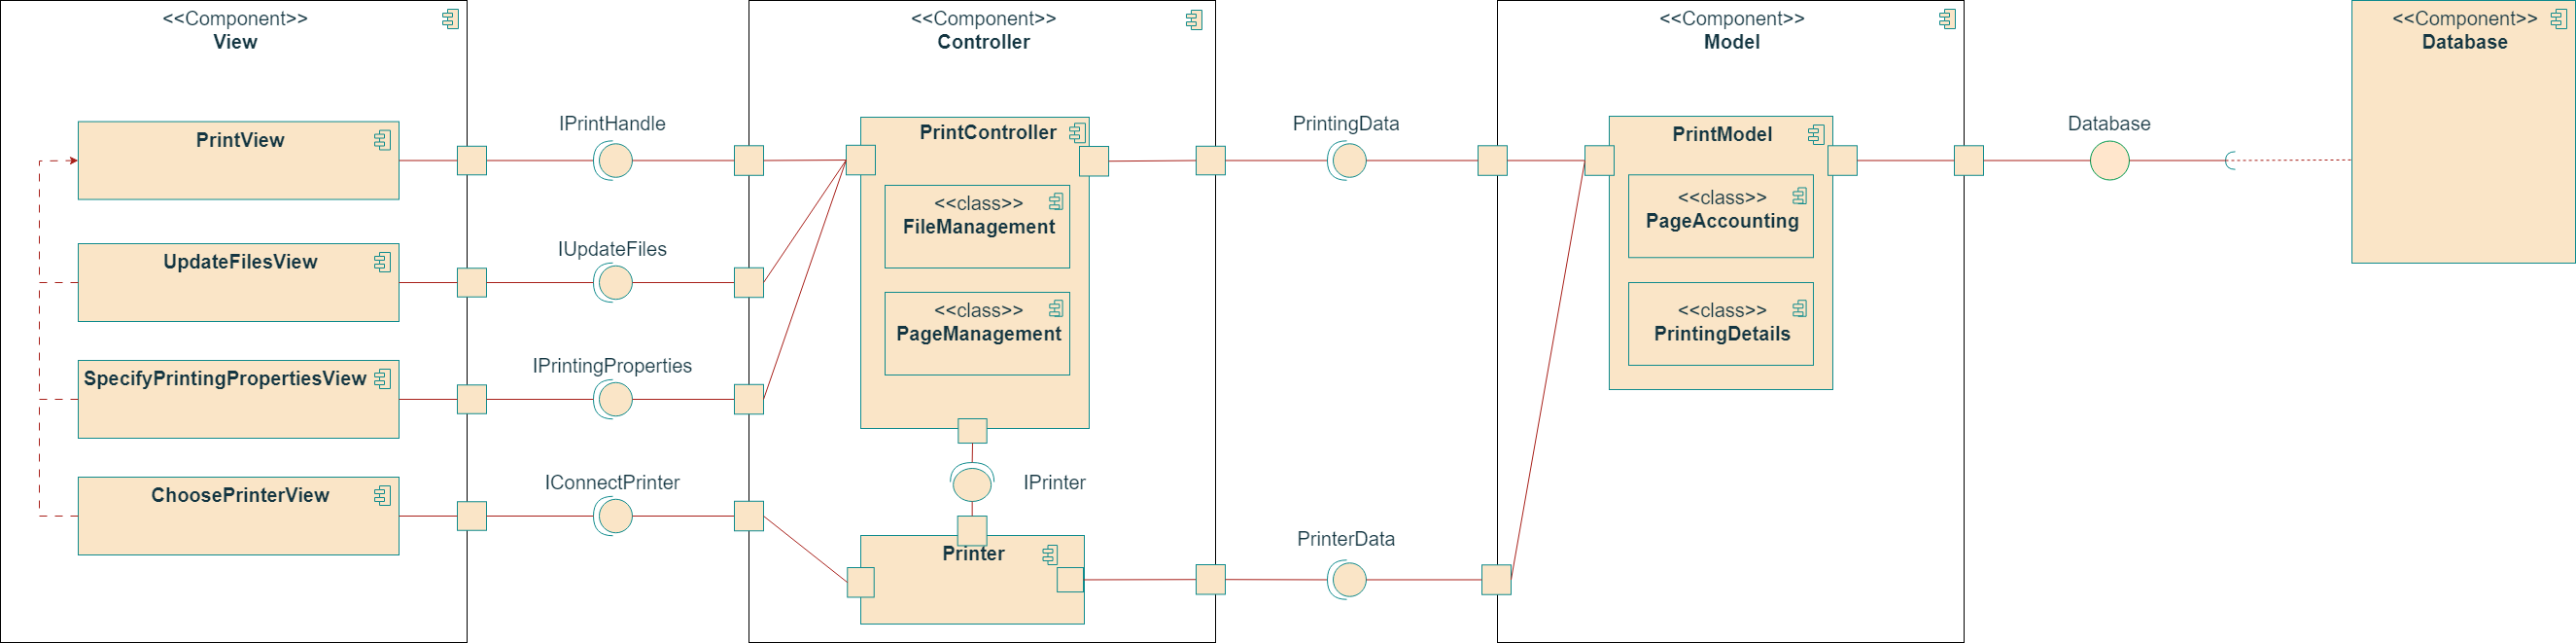
\includegraphics[width=16cm]{picture/3.2.Component_Print.drawio.png}
\caption{Component Diagram cho module in}
\end{center}
\end{figure}
\noindent \textbf{Mô tả}

\noindent \textbf{a. Component}

\noindent \textbf{Chế độ xem thành phần}
\begin{itemize}
    \item PrintView: Dùng để hiển thị UI chức năng in của Sinh viên. PrintView cần sử dụng Required Interface IPrintHandle
    \item UpdateFilesView, SpecifyPrintingPropertiesView, ChoosePrinterView: Đây là các Component phụ thuộc vào Component PrintView, dùng để hiển thị các chức năng cập nhật files, chọn máy in, xác định thông số tùy chỉnh in ấn trước khi in của Sinh viên. Trong đó UpdateFilesView cần sử dụng Required Interface IUpdateFiles, SpecifyPrintingPropertiesView cần sử dụng Required Interface IPrintingProperties, ChoosePrinterView cần sử dụng Required Interface IConnectPrinter
\end{itemize}

\noindent \textbf{Kiểm soát thành phần}
\begin{itemize}
    \item PrintController: Dùng để thực hiện chức năng in của Sinh viên thông qua tương tác với người dùng ở tầng trên và giao tiếp với Database ở tầng dưới. PrintController cần sử dụng Required Interface PrintingDatabase và cung cấp Provided Interface IPrintHandle. PrintController bao gồm 2 class FileManagement dùng để quản lý File và PageManagement dùng để quản lý số trang.
    \item Printer: Dùng để thao tác quản lý máy in. Printer  cung cấp Provided Interface IPrinter  và IConnectPrinter. Printer cần sử dụng Required Interface PrinterData.
\end{itemize}
\noindent \textbf{Mô hình thành phần}
\begin{itemize}
    \item PrintModel: Dùng để cập nhật và thao tác trên các dữ liệu về in ấn lấy trực tiếp từ Database. PrintModel bao gồm 2 class PageAccounting dùng để thực hiện các thao tác tính toán trên số trang và PrintingDetails để lấy ra các thông số, dữ liệu thống kê về in ấn. PrintModel cần truy cập để lấy dữ liệu từ Database để cung cấp cho tầng trên.
\end{itemize}

\noindent \textbf{b. Interface}
%%%%
\begin{table}[h!]
\centering
\begin{tabular}{|M{3cm}|p{6cm}|p{5.5cm}|}
\hline
\textbf{Tên interface} & \textbf{Chức năng} & \textbf{Các phương thức} \\
\hline
IPrintHandle & Dùng để xử lý các yêu cầu, thao tác in ấn từ Sinh viên. &  printRequest(username), checkValidPages(username)\\
\hline
IUpdateFiles & Dùng để xử lý các yêu cầu, thao tác cập nhật files từ Sinh viên. &  updateFile(file), removeFile(file), choosefile(filename) \\
\hline
IPrintingProperties & Dùng để xử lý các yêu cầu, thao tác về tùy chỉnh thông số in ấn từ Sinh viên. & selectProperties(properties) \\
& &  \\
\hline
IConnectPrinter & Dùng để xử lý các yêu cầu, thao tác chọn máy in và kết nối máy in từ Sinh viên. &  addPrinter(printer), deletePrinter(printer), updateOnPrinter(printer), updateOffPrinter(printer)\\
\hline
PrintingData & Dùng để truy cập vào dữ liệu liên quan đến việc in ấn & getSelectedProperties(), getPages(), getUploadedFiles() \\
PrinterData & Dùng để truy cập vào dữ liệu về máy in & getPrinterList() \\
\hline
\end{tabular}
\end{table}


% \noindent \textbf{b. Interface}

% \noindent \textbf{Interface IPrintHandle}: Dùng để xử lý các yêu cầu, thao tác in ấn từ Sinh viên.

% \noindent \textbf{Interface IUpdateFiles}: Dùng để xử lý các yêu cầu, thao tác cập nhật files (Chọn, Xóa files,...) từ Sinh viên.

% \noindent \textbf{Interface IPrintingProperties}: Dùng để xử lý các yêu cầu, thao tác về tùy chỉnh thông số in ấn từ Sinh viên.

% \noindent \textbf{Interface IConnectPrinter}: Dùng để xử lý các yêu cầu, thao tác chọn máy in và kết nối máy in từ Sinh viên.

% \noindent \textbf{Interface PrintingData}: Dùng để cung cấp dữ liệu in ấn cho các thao tác liên quan đến quản lý in ấn.

% \noindent \textbf{Interface PrinterData}: Dùng để cung cấp dữ liệu của máy in cho các thao tác liên quan đến quản lý máy in.

\subsubsection{Component Diagram của chức năng Xem số trang dư trong module In}
\begin{figure}[h!]
\begin{center}
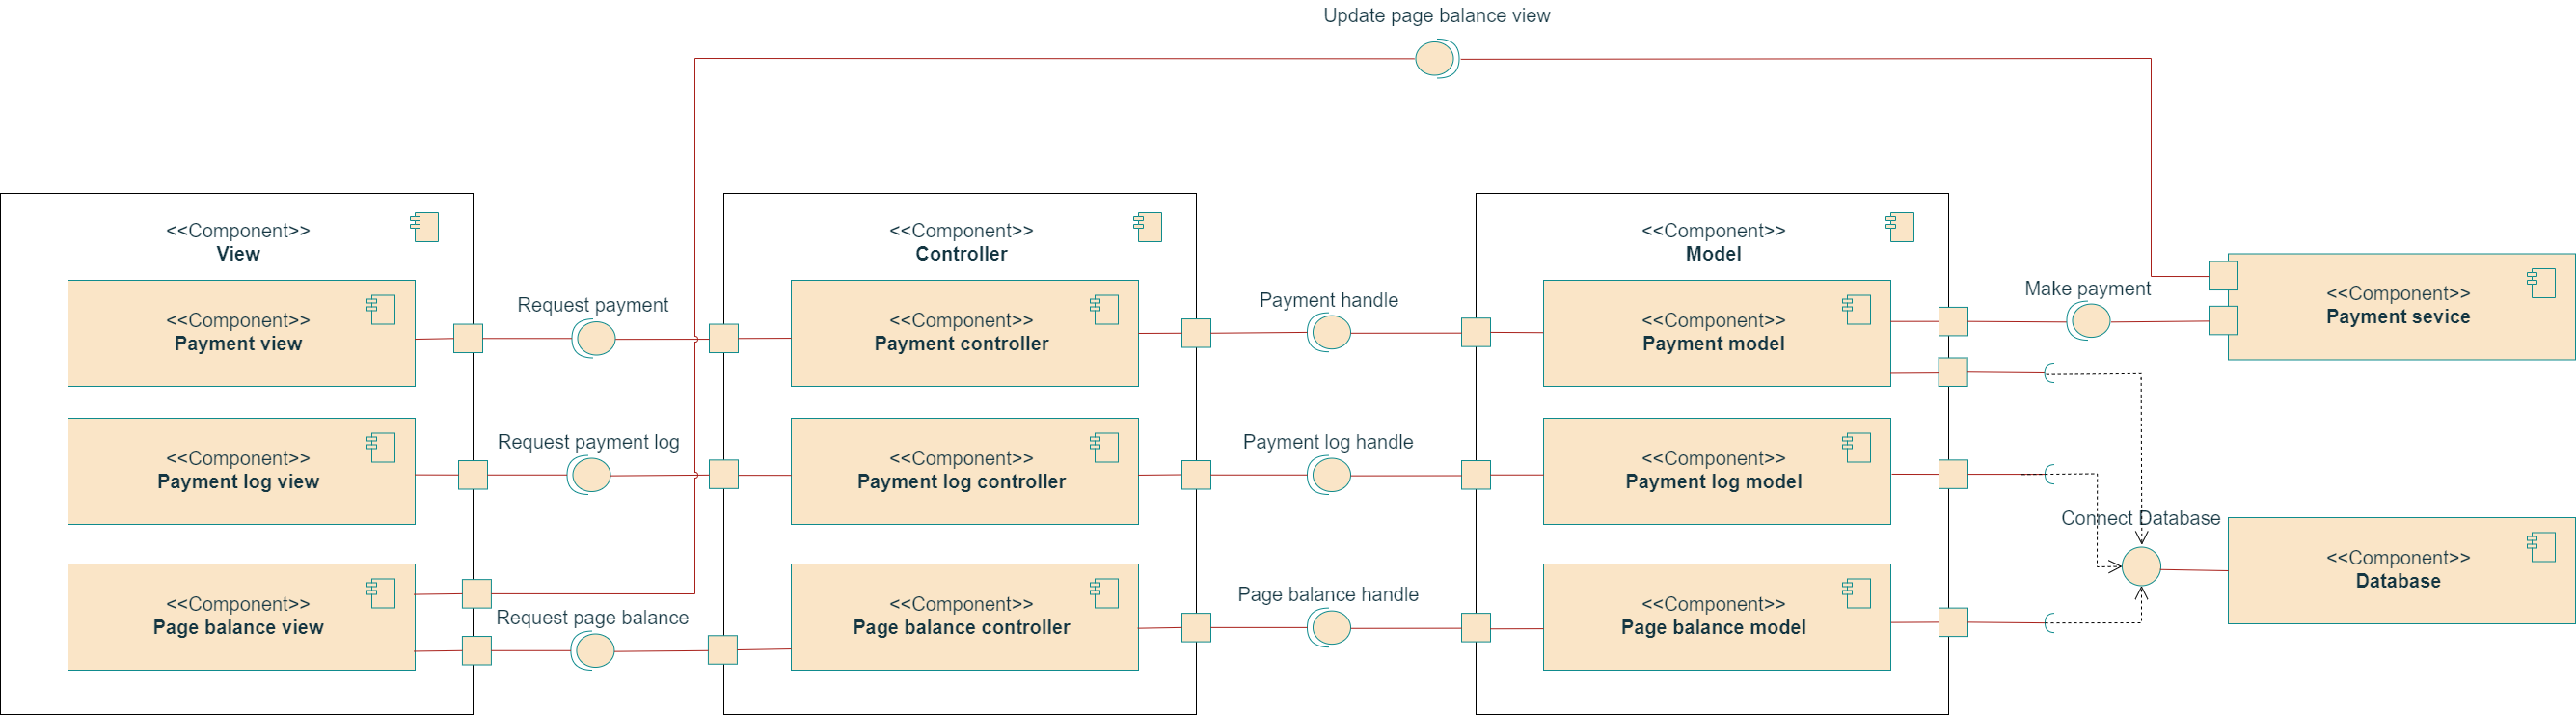
\includegraphics[width=16cm]{picture/Buy + view printing page.drawio (2).png}
\caption{Component Diagram for module xem số dư trang}
\end{center}
\end{figure}
\noindent \textbf{Mô tả}

\noindent \textbf{a. Component}

\noindent \textbf{Chế độ xem thành phần}
\begin{itemize}
    \item Payment view: Dùng để hiển thị UI chức năng mua thêm trang in của Sinh viên. Payment view cần sử dụng Required Interface Request payment.
    \item Payment log view: Dùng để hiển thị UI chức năng xem lịch sử mua trang in Sinh viên. Payment log view cần sử dụng Required Interface Request payment log.
    \item Page balance view: Dùng để hiển thị UI chức năng xem số trang in còn lại của Sinh viên. Page balance view cần sử dụng Required Interface Request page balance \& Update page blance view.
\end{itemize}

\noindent \textbf{Kiểm soát thành phần:}
\begin{itemize}
    \item Payment controller: Dùng để nhận các yêu cầu thanh toán từ người dùng, xử lí logic và tương tác với Payment model để lấy dữ liệu từ data base và tương tác với Payment service. 
    \item Payment log controller: Dùng nhận các yêu cầu xem lịch sử giao dịch từ người dùng, xử lí logic tương tác với Payment log model để lấy dữ liêu từ data base.
    \item Page balance controller: Dùng để nhận các yêu cầu xem số trang in còn lại, xử lí logic tương tác với Page balance model để lấy đữ liệu từ data base.
\end{itemize}
\noindent \textbf{Mô hình thành phần:}
\begin{itemize}
    \item Payment model: Nhận các yêu cầu từ controller, truy cập cập data base để truy xuất, cập nhật, và tương tác với payment service để thực hiện các giao dịch mua trang in sau đó controller sẽ trả kết quả về cho Payment view.
    \item Payment log model: Nhận các yêu cầu từ controller, truy cập data base để truy xuất lịch sử giao dịch, sau đó controller trả kết quả về cho Payment log view để hiển thị cho người dùng.
     \item Page balance model: Nhận các yêu cầu từ controller, truy cập data base để truy xuất số trang in hiện tại, sau đó controller trả kết quả về cho Page balance view để hiển thị cho người dùng.
\end{itemize}

\noindent \textbf{b. Interface}
%%%%
\begin{table}[h!]
\centering
\begin{tabular}{|M{3cm}|p{6cm}|p{5.5cm}|}
\hline
\textbf{Tên interface} & \textbf{Chức năng} & \textbf{Các phương thức} \\
\hline
Interface Request payment & Dùng để xử lý các yêu cầu mua thêm giấy in của Sinh viên. & \\
\hline
Interface Request payment log & Dùng để xử lý các yêu cầu xem lịch sử mua giấy in của Sinh viên. &  \\
\hline
Interface Request page balance & Dùng để xử lý các yêu cầu xem số trang in còn lại của Sinh viên. & \\
\hline
Interface Make payment & Dùng để kết nối với các cổng thanh toán bên ngoài. &  \\
\hline
Interface Payment log handle & Dùng để cung cấp dữ liệu liên quan đến lịch sử giao dịch. & \\
\hline
Interface Page balance handle & Dùng để cung cấp dữ liệu liên quan đến số trang in còn lại. &  \\
\hline
Interface Payment handle & Dùng để cung cấp dữ liệu liên quan đến thanh toán. & \\
\hline
Interface Connect Database & Dùng để truy cập vào cơ sở dữ liệu & \\
\hline
\end{tabular}
\end{table}

\newpage
\section{Implementation - Sprint 1}
\subsection{Github}
\noindent Nhóm tạo một Repository làm việc chung tại: \url{https://github.com/NguyenDuong163/SoftwareEngineer_Gr4}
\subsection{Kiểm tra sử dụng}
\subsubsection{Tuyển người tham gia}
\textit{Participants hay người tham gia trải nghiệm nên là những người dung tiềm năng của [trang web]. Họ có thể là những người đã từng trải nghiệm một số sản phẩm hoặc dịch vụ tương tự trước đây. Mặt khác, người tham gia nên là những người cần đến dịch vụ và lợi ích mà nó mang lại.}

\noindent \textbf{Mục tiêu và phạm vi tuyển người tham gia:}
\begin{itemize}
  \item \textbf{Mục tiêu:} Thu thập phản hồi thực tế từ trải nghiệm của người tham gia sử dụng \textit{[trang web]} để in tài liệu.
  
  \item \textbf{Phạm vi tuyển dụng:} Là các người dùng tiềm năng (sinh viên trong trường, giảng viên, ...), những người đã từng sử dụng các dịch vụ tương tự (học sinh, sinh viên trường khác,...).
\end{itemize}

\noindent \textbf{Phương pháp tuyển người tham gia:}
\begin{itemize}
  \item Qua email
  \item Qua các bài tuyển dụng được đăng trên các trang mạng xã hội lớn (Facebook, ...)
  \item Bạn bè; bạn chung lớp, chung khoa; ...
\end{itemize}

\noindent \textbf{Số liệu về người tham gia:}
\begin{itemize}
  \item \textbf{Số lượng người tham gia trải nghiệm} \textit{[trang web]} \textbf{dự kiến:} 5-7 người (\url{https://www.nngroup.com/articles/why-you-only-need-to-test-with-5-Người dùngs/})
  
  \item \textbf{Đặc điểm chung của người tham gia:} Có kiến thức cơ bản về máy tính; biết hoặc thường xuyên sử dụng web; biết các thuộc tính khi in tài liệu. Không yêu cầu đặc biệt về độ tuổi, giới tính hay chuyên ngành hoặc nghề nghiệp.
\end{itemize}
\newpage
\subsubsection{Xác định các nhiệm vụ}
% \textbf{Tương tác cơ bản với [trang web]}
% \begin{figure}[h!]
% \begin{center}
% 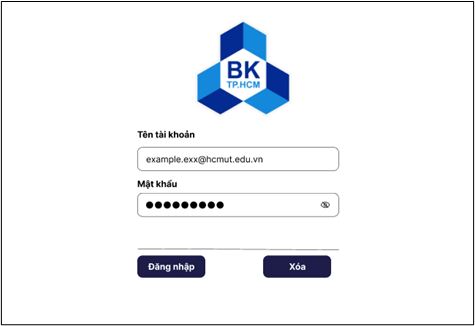
\includegraphics[width=8cm]{login.png}
% \caption{Trang đang nhập của trang web}
% \end{center}
% \end{figure}
% \begin{enumerate}
%   \item Truy cập \textit{[trang web]} và thực hiện đăng nhập.
%   \item Xem lịch sử in.
%   \item Xem lịch sử giao dịch.
%   \item Xem hướng dẫn sử dụng.
%   \item Đăng xuất tài khoản đang dùng.
% \end{enumerate}

% \textbf{Sử dụng chức năng chính của [trang web]}
% \begin{figure}[h!]
% \begin{center}
% 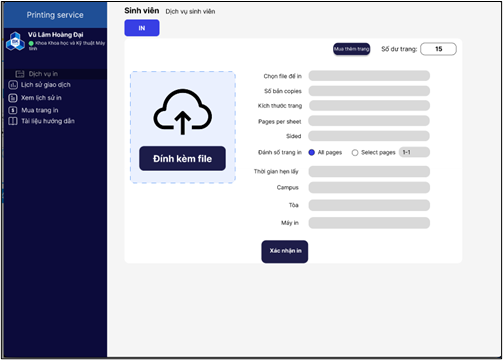
\includegraphics[width=8cm]{mainpage.png}
% \caption{Trang chính của trang web}
% \end{center}
% \end{figure}
% \begin{enumerate}
%   \item Thực hiện in một file pdf (cho trước) theo chế độ in mặc định.
%   \item Chọn một file pdf và chọn lại một file pdf khác và thực hiện in với khổ giấy A3.
%   \item Thực hiện in một file word (cho trước) với số trang phải in lớn hơn số dư trang.
%   \item Khi xuất hiện lỗi không đủ trang in, xử lý lỗi và tiếp tục in.
%   \item Mua thêm 10 trang in và thanh toán qua Momo.
%   \item In một file pdf (cho trước) từ trang 1-9 và in hai mặt, hẹn lấy 30 phút sau in.
%   \item Xem lịch sử in sau mỗi lần in.
% \end{enumerate}

% \textbf{Open-ended tasks}
% \begin{enumerate}
%   \item Thao tác với \textit{[trang web]} liên tục trong 5 phút.
%   \item Dùng \textit{[trang web]} trong 5 phút và in được 2 file pdf bất kì.
%   \item Mua trang in và thực hiện thanh toán trước khi hết thời gian thanh toán.
% \end{enumerate}
\subsubsubsection{Chức năng in}
\begin{table}[h!]
\centering
\begin{tabularx}{\textwidth}{|s|X|X|X|}
\hline
 \textbf{Tên testcase:} & In & Mã testcase & TC\_01 \\ \hline
 \textbf{Được tạo bởi:} & Vũ Lâm Hoàng Đại  & Cập nhật lần cuối: &  Vũ Lâm Hoàng Đại\\ \hline
 \textbf{Ngày tạo} & 18/11/2023  & Ngày cập nhật cuối & 19/11/2023\\ \hline
 \textbf{Mô tả:} &  \multicolumn{3}{p{10cm}|}{Người kiểm thử thực hiện chức năng in với các cửa sổ được hiện lên đầy đủ} \\ \hline
 \textbf{Mức độ quan trọng:} &  \multicolumn{3}{l|}{Cao} \\ \hline

 \textbf{Tiền điều kiện:} &  \multicolumn{3}{p{10cm}|}{Kết nối Internet khả dụng.
Khách hàng đã đăng nhập vào hệ thống
} \\ \hline
 \textbf{Kết quả mong đợi:} &  \multicolumn{3}{l|}{Màn hình xác nhận in thành công với 100\% mức độ hoàn thành}\\ \hline
 \textbf{Các luồng:} &  \multicolumn{3}{l|}
 {\begin{tabular}[t]{@{}p{10cm}@{}}
1. Sau khi đã đăng nhập, tester chọn "Dịch vụ in" trên sidebar  \\
2. Tester bấm vào nút ”đính kèm files”.\\
3. Cửa sổ hệ thống hiện ra, tester tiến hành chọn file mình muốn in. \\
4. Tại màn hình bên phải, tester tiến hành nhập các trường thông tin cần thiết để chuẩn bị in\\
5. Tester bấm xác nhận in\\
6. Màn hình chuyển thành quá trình đang in file với mức độ hoàn thành là 100\%. \\
7. Tester bấm vào “In hoàn tất” để hoàn tất công việc in\\
\end{tabular}} \\ \hline
 
\textbf{Ngoại lệ:} &  \multicolumn{3}{l|}{\begin{tabular}[t]{@{}p{10cm}@{}}
 - Tại bước 3, nếu tester chọn file ngoại lệ với file cho phép của hệ thống, một cửa sổ lỗi sẽ hiện ra và yêu cầu tester thực hiện lại bước 3.\\
 - Tại bước 4, nếu tester nhập không đủ một số trường bắt buộc, hệ thống sẽ hiện lên cảnh báo và yêu cầu tester nhập hết\\
 - Tại bước 5, nếu tester bấm thực hiện in cho một file có số trang lớn hơn số dư trang hiện có của tài khoản test (được đặt mặc định là 15) thì một cửa sổ hiện lên yêu cầu tester chuyển đến chức năng thanh toán\\ 
\end{tabular}}  \\ \hline
\textbf{Tài liệu đính kèm:} &  \multicolumn{2}{l}{} & \\ \hline
\end{tabularx}
\end{table}
\newpage
\begin{table}[h!]
\centering
\begin{tabular}{|c|c|}
\hline
\textbf{Màn hình flow} & 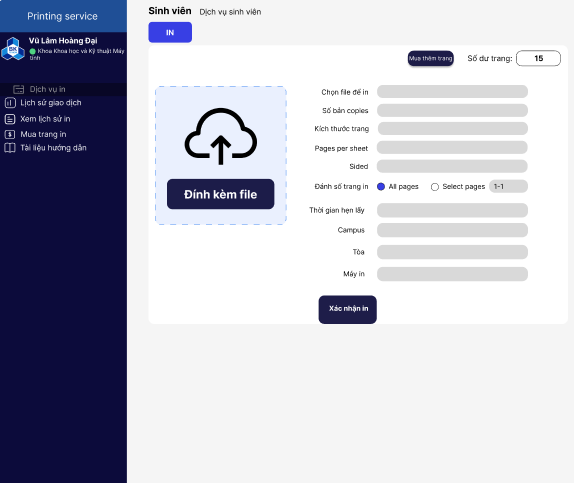
\includegraphics[width=7cm]{picture/pic1-1.png} \\ & 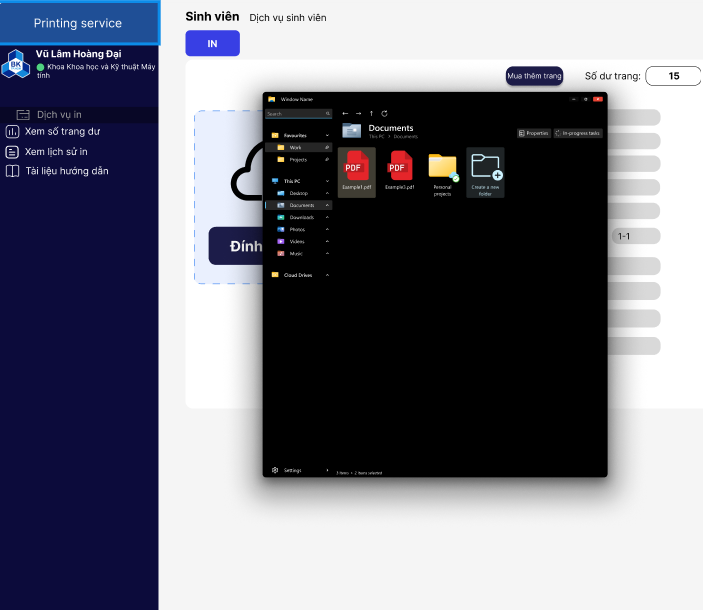
\includegraphics[width=7cm]{picture/pic2-2.png}\\ & 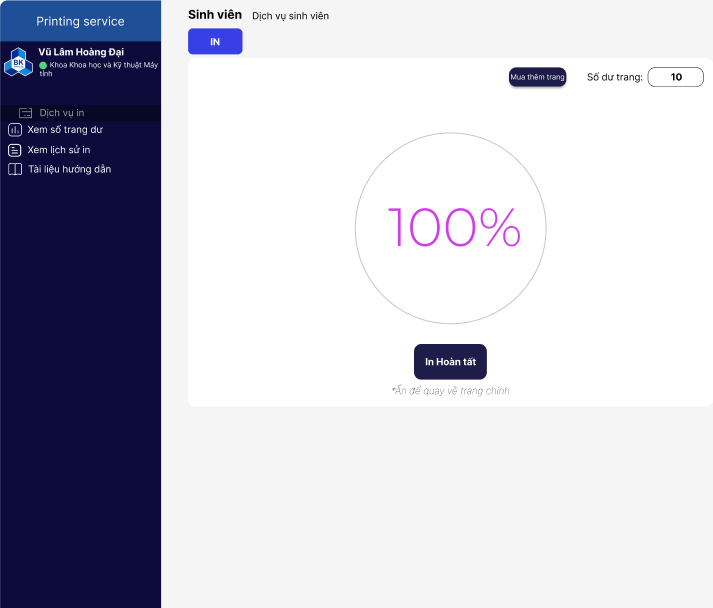
\includegraphics[width=7cm]{picture/pic3-3.png}\\
\hline
\end{tabular}
\end{table}
\newpage
\begin{table}[h!]
\centering
\begin{tabular}{|c|c|}
\hline
\textbf{Màn hình ngoại lệ} & 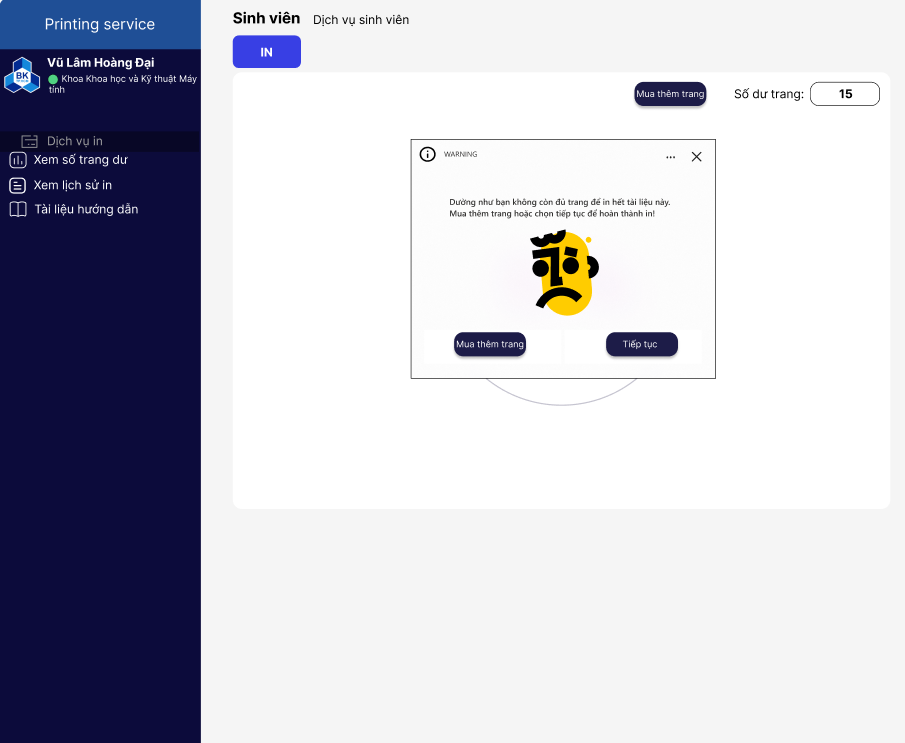
\includegraphics[width=7cm]{picture/pic4-4.png} \\ 
\hline
\end{tabular}
\end{table}
\newpage
\subsubsubsection{Chức năng mua thêm trang}
\begin{table}[h!]
\centering
\begin{tabularx}{\textwidth}{|s|X|X|X|}
\hline
 \textbf{Tên testcase:} & Mua trang in & Mã testcase & TC\_02 \\ \hline
 \textbf{Được tạo bởi:} & Vũ Lâm Hoàng Đại  & Cập nhật lần cuối: &  Vũ Lâm Hoàng Đại\\ \hline
 \textbf{Ngày tạo} & 18/11/2023  & Ngày cập nhật cuối & 19/11/2023\\ \hline
 \textbf{Mô tả:} &  \multicolumn{3}{p{10cm}|}{Người kiểm thử thực hiện mua thêm trang với các cửa sổ được hiện lên đầy đủ} \\ \hline
 \textbf{Mức độ quan trọng:} &  \multicolumn{3}{l|}{Cao} \\ \hline

 \textbf{Tiền điều kiện:} &  \multicolumn{3}{p{10cm}|}{Kết nối Internet khả dụng.
Khách hàng đã đăng nhập vào hệ thống
} \\ \hline
 \textbf{Kết quả mong đợi:} &  \multicolumn{3}{l|}{Số trang in sau khi đã mua được cộng vào trong tài khoản}\\ \hline
 \textbf{Các luồng:} &  \multicolumn{3}{l|}
 {\begin{tabular}[t]{@{}p{10cm}@{}}
1. Sau khi đã đăng nhập, tester chọn "Mua trang in" trên sidebar  \\
2. Cửa sổ hiện lên với số dư trang hiện có( mặc định của tài khoản tester là 15)\\
3. Tester nhấn chọn “Mua trang” \\
4. Tester nhập số trang muốn mua thêm, hệ thống sẽ tính toán và trả về số tiền cần phải trả cho việc mua trang\\
5. Tester chọn phương thức thanh toán\\
6. Tester chọn nút “Thanh toán” \\
7. Hệ thống chuyển qua trang web tương ứng với phương thức thanh toán tester đã chọn( mặc định khi test sẽ chuyển qua trang thanh toán qua phương thức momo) và tiến hành thanh toán( khi test tiền phải thanh toán cho hệ thống sẽ là 0 đồng)\\
8. Online payment providers xác thực thanh toán và hệ thống cập nhật số trang in cho tài khoản tester\\

\end{tabular}} \\ \hline
 
\textbf{Ngoại lệ:} &  \multicolumn{3}{l|}{\begin{tabular}[t]{@{}p{10cm}@{}}
 - Tại bước 6, nếu số trang muốn mua vượt quá 999, hệ thống sẽ không cho phép tester thực hiện thanh toán\\
\end{tabular}}  \\ \hline
\textbf{Tài liệu đính kèm:} &  \multicolumn{2}{l}{} & \\ \hline
\end{tabularx}
\end{table}
\newpage
\begin{table}[h!]
\centering
\begin{tabular}{|c|c|}
\hline
\textbf{Màn hình flow} & 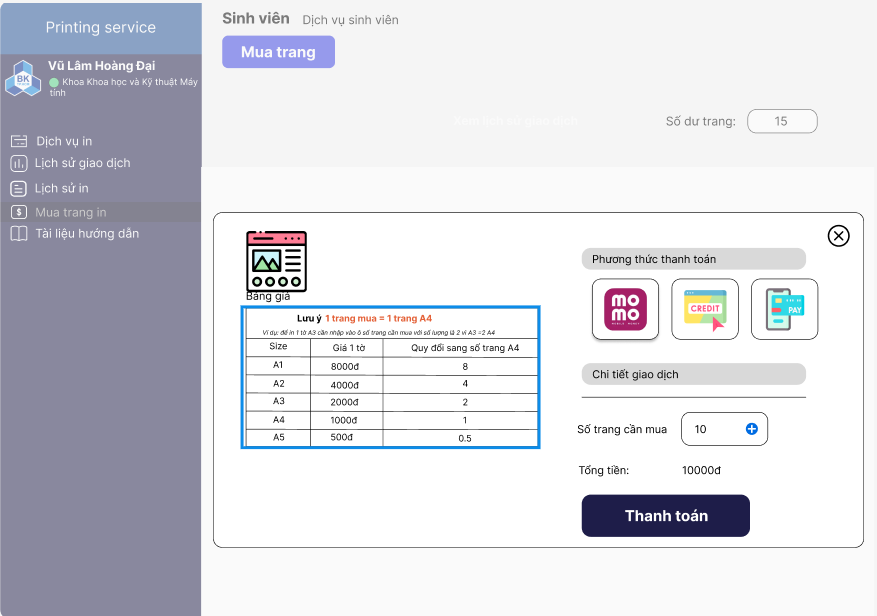
\includegraphics[width=7cm]{picture/pic5-5.png} \\ & 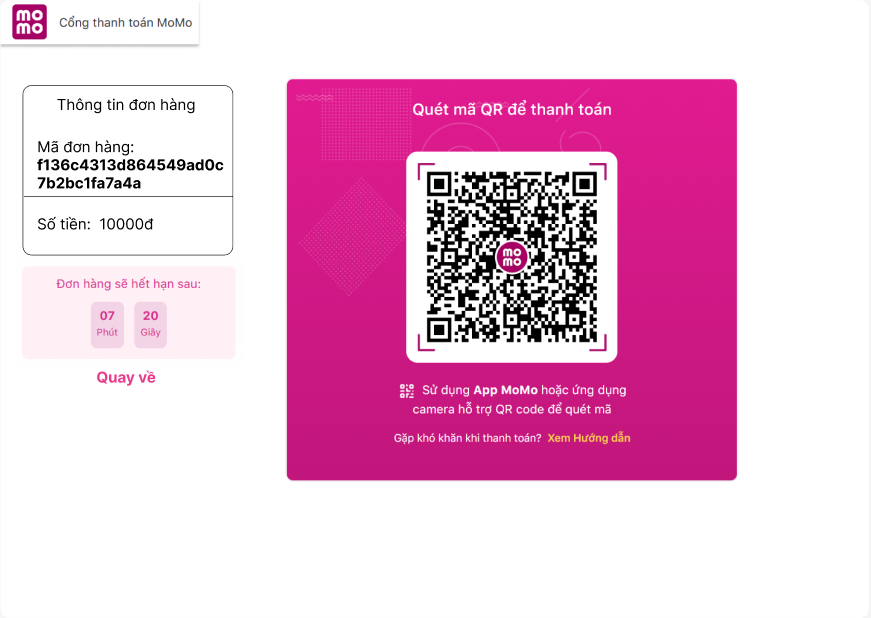
\includegraphics[width=7cm]{picture/pic6-6.png}\\
\hline
\end{tabular}
\end{table}
\subsubsection{Xác định chiến lược kiểm thử}
\subsubsubsection{Phân tích định tính}
Đối với thử nghiệm khả năng sử dụng của dịch vụ in thông minh dành cho sinh viên HCMUT (HCMUT\_SSPS), nhóm sẽ sử dụng phương pháp tiếp cận chất lượng. Nghĩa là nhóm sẽ quan tâm nhiều hơn đến việc hiểu trải nghiệm của người dùng hơn là thu thập dữ liệu số. Một phần cũng là do giai đoạn kiểm nghiệm gấp rút không thể phần tích theo hướng định lượng được.\\
Nhóm sẽ quan sát người tham gia khi họ sử dụng hệ thống và đặt câu hỏi mở để lấy ý kiến của những người tham gia.\\
Phương pháp tiếp cận định lượng sẽ phù hợp hơn nếu nhóm quan tâm đến việc đo lường các khía cạnh cụ thể của hệ thống, chẳng hạn như thời gian hoàn thành một việc in thành công một file cho người dùng tải lên hoặc số lỗi xảy ra. Tuy nhiên, đối với thử nghiệm ban đầu này, nhóm muốn tập trung vào việc hiểu cách người dùng tương tác với hệ thống và xác định bất kỳ vấn đề khả năng sử dụng lớn nào.
\subsubsubsection{Thử nghiệm từ xa}
Nhóm sẽ thực hiện thử nghiệm khả năng sử dụng từ xa. Nghĩa là người tham gia sẽ sử dụng hệ thống tại trường hoặc tại bất cứ đâu. Và người kiểm thử vẫn tham gia vào việc yêu cầu các nhiệm vụ cho người tham gia thông qua Google Meet. Thử nghiệm từ xa thường thuận tiện hơn cho người tham gia và có thể ít tốn kém hơn so với thử nghiệm trực tiếp. Mặc dù vẫn kết việc mở camera để thấy người tham gia nhưng có thể khó khăn hơn để quan sát ngôn ngữ cơ thể và biểu cảm trên khuôn mặt của người tham gia, điều này có thể cung cấp những hiểu biết có giá trị về trải nghiệm của họ. Vì thế sau khi người dùng kiểm thử phần mềm nhóm sẽ thực hiện một form để thu thập về feedback của người tham gia.\\
Nhóm đã quyết định thực hiện thử nghiệm từ xa vì nhóm muốn tiếp cận một nhóm người tham gia rộng lớn hơn, bao gồm cả những sinh viên có thể không đến được trường để tham gia thử nghiệm trực tiếp. Nhóm cũng sẽ có thể thử nghiệm người tham gia trên thiết bị của họ, điều này sẽ giúp chúng tôi xác định bất kỳ vấn đề khả năng sử dụng cụ thể cho thiết bị nào.\\
\textbf{Kế hoạch thực hiện: }
\begin{enumerate}
\item \textbf{Chọn một công cụ để giao tiếp với người tham gia}
\begin{itemize}
\item Google Meeting
\item Thông báo cho những người tham gia về việc sẽ sử dụng Google Meeting làm công cụ để giao tiếp và cài sẵn công cụ để ghi màn hình.
\item Thông báo cho họ sẽ yêu cầu về camera cũng như máy tính có thể chia sẻ màn hình, ghi màn hình.
\end{itemize}

\item \textbf{Giao nhiệm vụ:}
\begin{itemize}
\item Gửi cho người tham gia một file tóm tắt các task sẽ được thực hiện để đọc trước
\end{itemize}

\item \textbf{Buổi meeting:}
\begin{itemize}
\item Mời tất cả người tham gia và những người kiểm thử vào meet.
\item Meeting với các câu hỏi. Ví dụ:
\begin{enumerate}
\item Xin chào mọi người
\item Sau đây mình xin đếm đủ số lượng người tham gia đã vào đủ hay chưa ?
\item Các bạn đã bật ghi hình chưa ?
\end{enumerate}
\end{itemize}

\item \textbf{Kết thúc buổi kiểm thử}
\begin{itemize}
\item Cảm ơn người tham gia
\item Dừng ghi màn hình và gửi form feedback cho người tham gia điền vào.
\end{itemize}

\end{enumerate}
\subsubsection{Hồ sơ các cá nhân tham gia kiểm thử}
\textbf{ Đặc điểm các cá nhân tham gia: }\\
- Có kiến thức cơ bản về máy tính;\\ 
- Biết hoặc thường xuyên sử dụng web;\\
- Biết đến các chức năng và tính năng in.\\
- Không yêu cầu đặc biệt về độ tuổi, giới tính hay chuyên ngành hoặc nghề nghiệp\\
\textbf{ Bảng chi tiết cá nhân tham gia }
\begin{table}[]
\begin{tabular}{|l|l|l|l|}
\hline
STT & Tuổi & Giới tính & Nghề nghiệp     \\ \hline
1   & 16   & Nam       & Học sinh cấp 3  \\ \hline
2   & 20   & Nữ        & Sinh viên năm 3 \\ \hline
3   & 20   & Nam       & Sinh viên năm 3 \\ \hline
4   & 19   & Nam       & Sinh viên năm 2 \\ \hline
5   & 42   & Nữ        & Giảng viên      \\ \hline
\end{tabular}
\end{table}
\subsubsection{Kết quả kiểm thử}
\subsubsubsection{Kết quả kiểm thử }
Bảng đánh giá Usability Scale (SUS) cho kết quả như sau
Bảng đánh giá được cho với thang đo từ 1 đến 5 với 1 là Hoàn toàn không hài lòng và 5 là hoàn toàn hài lòng
\begin{longtable}{|c|p{7cm}|*{5}{c|}}
\hline
STT & \multicolumn{1}{c|}{Tiêu chuẩn đánh giá} & 1 & 2 & 3 & 4 & 5 \\ \hline
\endfirsthead

\multicolumn{7}{c}%
{{\bfseries \tablename\ \thetable{} -- Tiếp tục từ trang trước}} \\
\hline
STT & \multicolumn{1}{c|}{Tiêu chuẩn đánh giá} & 1 & 2 & 3 & 4 & 5 \\ \hline
\endhead

\hline \multicolumn{7}{|r|}{{Tiếp tục sau trang sau}} \\ \hline
\endfoot

\hline
\endlastfoot

1 & Tôi nghĩ rằng tôi muốn sử dụng hệ thống này thường xuyên & & 1 & 3 & 1 & \\ \hline
2 & Tôi thấy hệ thống này phức tạp một cách không cần thiết & & 2 & 3 & & \\ \hline
3 & Tôi nghĩ hệ thống này rất dễ sử dụng & & 1 & & 3 & 1 \\ \hline
4 & Tôi nghĩ rằng tôi sẽ cần sự hỗ trợ của nhân viên kỹ thuật để có thể sử dụng hệ thống này & 4 & & & 1 & \\ \hline
5 & Tôi nhận thấy các chức năng khác nhau trong hệ thống này được tích hợp rất tốt & & & 3 & 2 & \\ \hline
6 & Tôi nghĩ có quá nhiều mâu thuẫn trong hệ thống này & & 2 & 2 & 1 & \\ \hline
7 & Tôi tưởng tượng rằng hầu hết mọi người sẽ học cách sử dụng hệ thống này rất nhanh & & 3 & 1 & 1 & \\ \hline
8 & Tôi thấy hệ thống này rất cồng kềnh khi sử dụng & & 2 & 2 & & 1 \\ \hline
9 & Tôi cảm thấy rất tự tin khi sử dụng hệ thống & & & 3 & & 2 \\ \hline
10 & Tôi cần phải học rất nhiều thứ trước khi có thể sử dụng hệ thống này. & 1 & 1 & 2 & 1 & \\ \hline

\end{longtable}
Điểm trung bình của báo cáo là : 74,75 ,đạt mức tốt trong thang đo.
\newpage
\subsubsubsection{Các vấn đề được chỉ ra}
\begin{table}[h!]
\centering
\begin{tabular}{|c|c|c|c|c|}
\hline
Mã vấn đề & Tên vấn đề & \multicolumn{3}{c|}{Độ quan trọng} \\
\cline{3-5}
& & Đối với tester & Đối với tổ chức & Tổng \\
\hline
P\_I\_01 & Giao diện không nhất quán & 5 & 4 & 9 \\
P\_F\_01 & Vấn đề lỗi trong quá trình in & 5 & 2 & 7 \\
P\_F\_02 & Hệ thống thanh toán khó chịu & 3 & 3 & 6 \\
P\_I\_02 & Lỗi hiện thị khi mua tràn số trang & 2 & 3 & 5 \\
P\_I\_03 & Khó hiểu trong các tùy chọn in & 3 & 1 & 4 \\
\hline
\end{tabular}
\end{table}
\subsubsubsection{ Phương hướng giải quyết}
\begin{table}[h!]
\centering
\begin{tabularx}{\textwidth}{|c|X|X|}
\hline
Mã vấn đề & Mô tả chi tiết & Phương hướng giải quyết \\
\hline
\makecell{P\_I\_01} & Giao diện thiết kế còn nhiều nút khó hiểu, các bố cục về sắp xếp khiến người dùng khó khăn khi sử dụng & {Đảm bảo thiết kế nhất quán trên toàn hệ thống, bao gồm vị trí đặt nút, cách phối màu và thuật ngữ.} \\
\hline
P\_F\_01 & Nếu xảy ra lỗi trong quá trình in, người dùng có thể không nhận được thông báo lỗi rõ ràng hay việc chờ quá lâu trong hàng in & Thực hiện xử lý lỗi hiệu quả bằng các thông báo mô tả, hướng dẫn cách giải quyết vấn đề và thông tin liên hệ để được hỗ trợ nếu cần.\\
\hline
P\_F\_02 & Hệ thống thanh toán khiến người dùng cần một số ứng dụng nhất định để thanh toán, đồng thời việc phải sử dụng đến một thiết bị thứ 3 để thanh toán & Tích hợp đa dạng nền tảng thanh toán hơn, đồng thời tinh giản quá trình thanh toán\\
\hline
P\_I\_02 & Khi tổng số trang trong tài khoản của người dùng trên 999, khiến cho vùng số dư trang không hiển thị hết được  & Thực hiện tính toán trước khi cho mua, nếu tổng số dư trang sau khi mua vượt 999 sẽ hiện cảnh báo\\
\hline
P\_I\_03 & Một số trường tùy chọn in còn khó hiểu với người mới, hay người không có kiến thức về in ấn & Bản tài liệu hướng dẫn cần hướng dẫn chi tiết về thuộc tính các trường cho người dùng thuận tiện sử dụng.\\
\hline
\end{tabularx}
\end{table}

\newpage
\subsection{Data Usage}
\subsubsection{Thiết kế lược đồ EERD}
\begin{figure}[h!]
    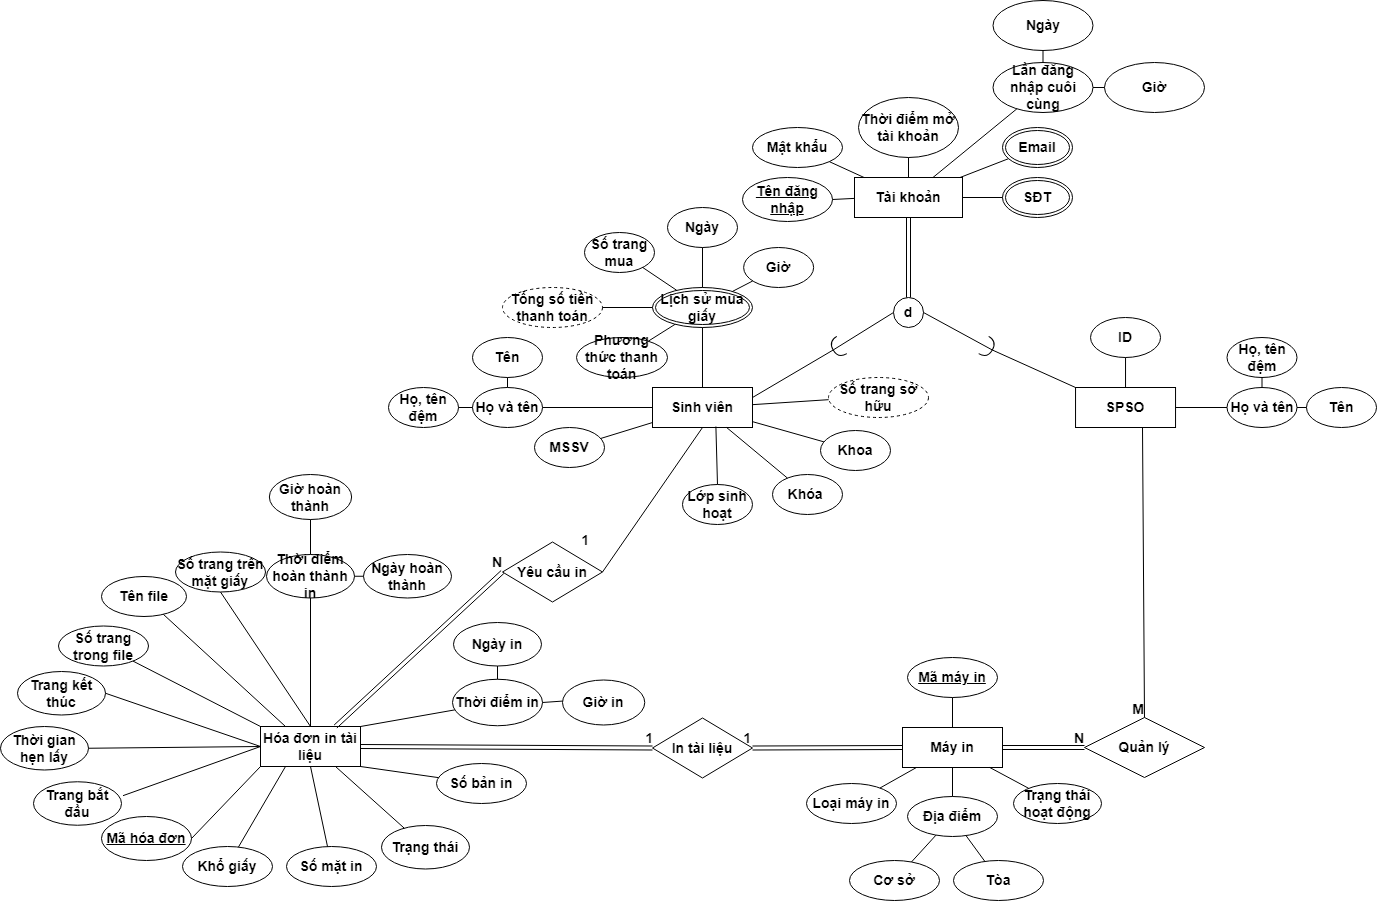
\includegraphics[scale = 0.35]{picture/eerd.png}
    \caption{Lược đồ EERD cho việc lưu trữ Database}
\end{figure}
\newpage
\subsubsection{Ánh xạ lược đồ quan hệ Relational Schema}
\begin{figure}[h!]
    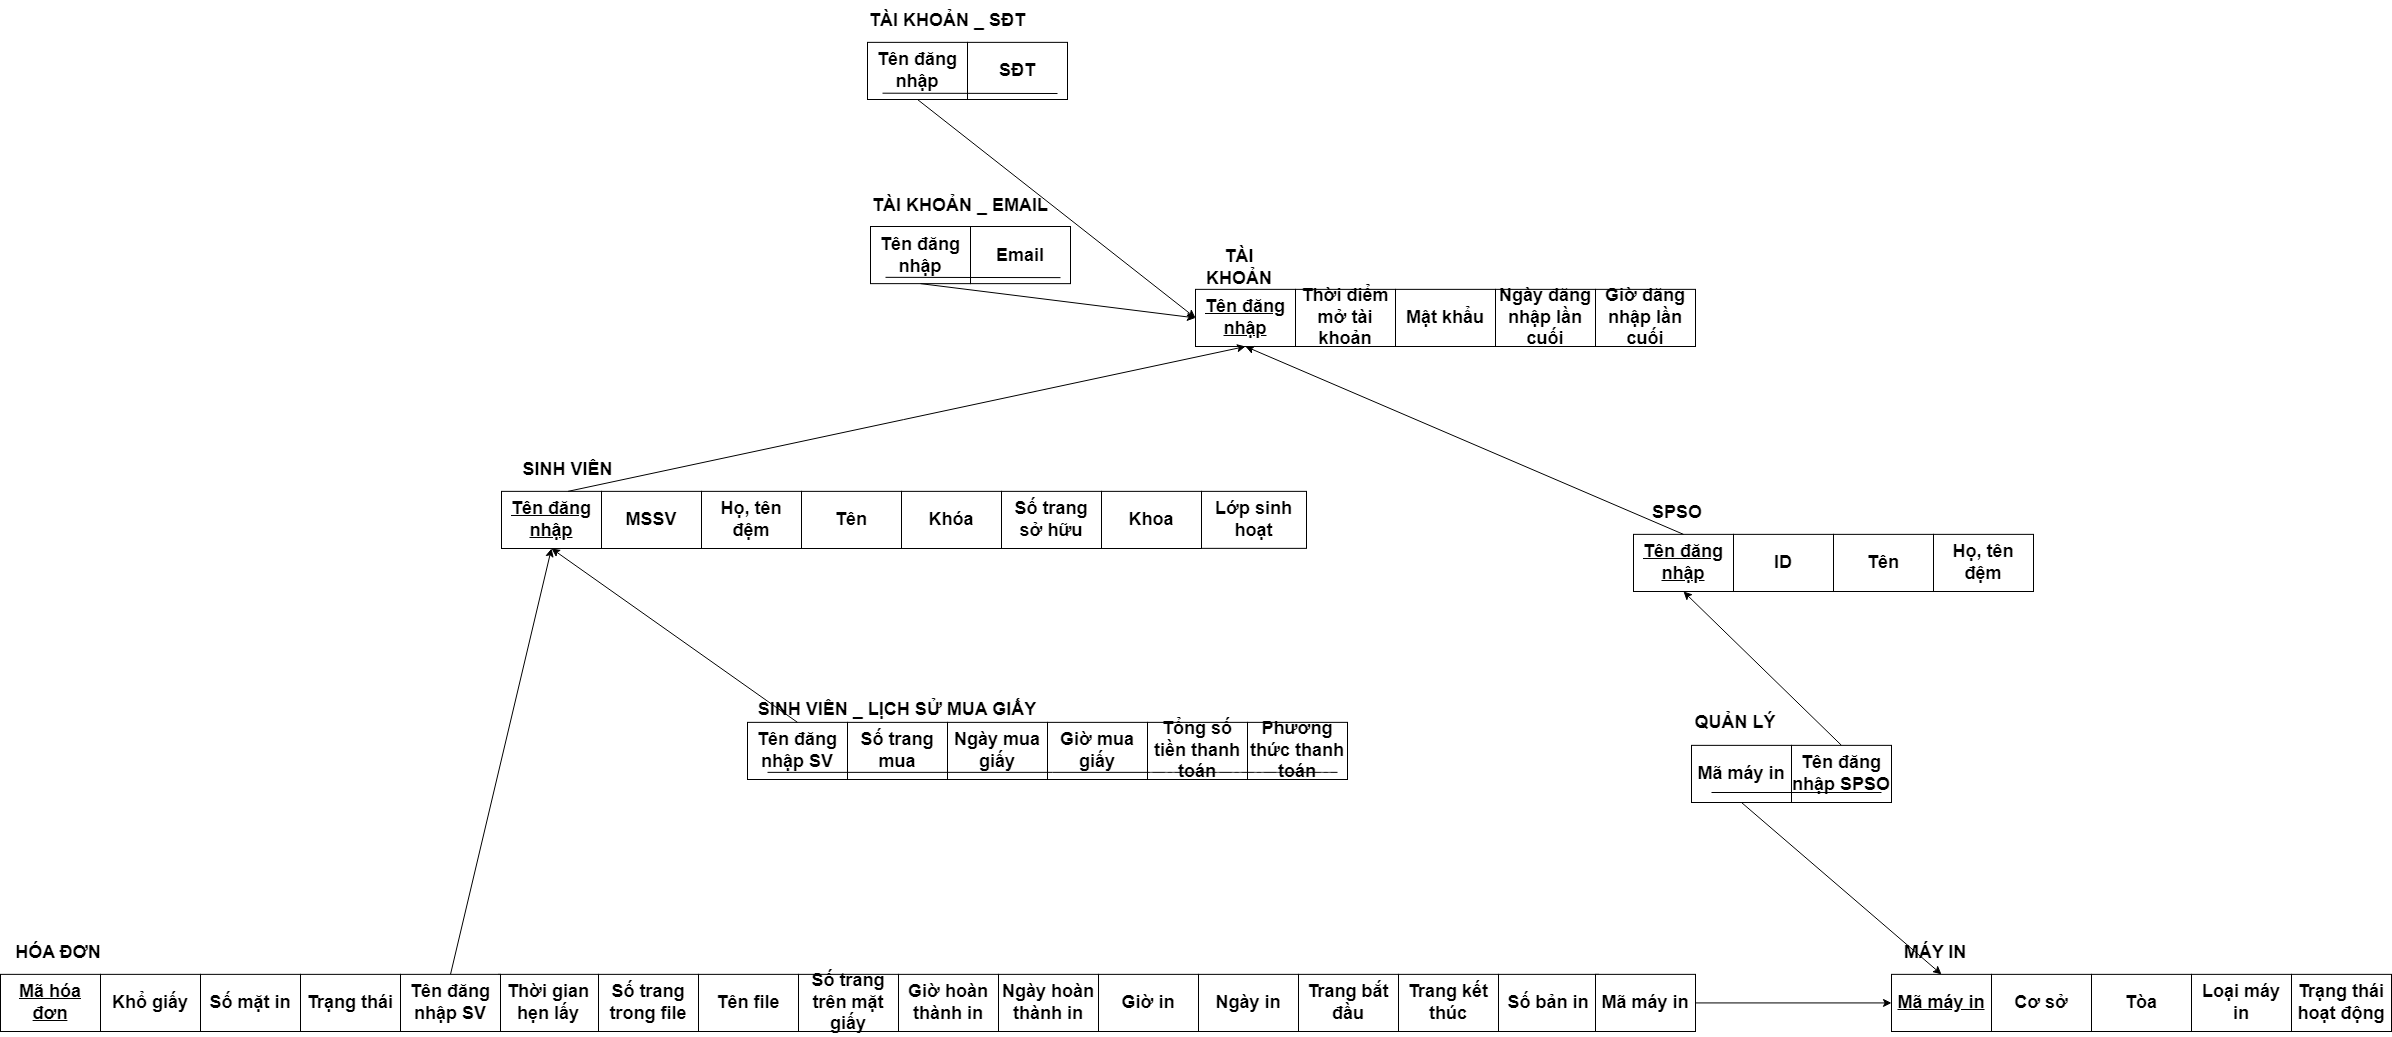
\includegraphics[scale = 0.2]{picture/relationalschema.png}
    \caption{Relational Schema ánh xạ từ EERD}
\end{figure}

\noindent \textbf{Mô tả lược đồ:}
\begin{itemize}
    \item TÀI KHOẢN\_SĐT: Bao gồm các thông tin \underline{Tên đăng nhập}, \underline{SĐT}
    \item TÀI KHOẢN\_EMAIL: Bao gồm các thông tin \underline{Tên đăng nhập}, \underline{Email}
    \item TÀI KHOẢN:Bao gồm các thông tin \underline{Tên đăng nhập}, Thời điểm mở tài khoản, Mật khẩu, Ngày đăng nhập lần cuối, Giờ đăng nhập lần cuối.
    \item SINH VIÊN: Bao gồm các thông tin \underline{Tên đăng nhập}, MSSV, Họ, tên đệm, Tên, Khóa, Số trang sở hữu, Khoa.
    \item SPSO: Bao gồm các thông tin \underline{Tên đăng nhập}, ID, Tên, Họ, tên đệm.
    \item SINH VIÊN\_LỊCH SỬ MUA GIẤY: Bao gồm các thông tin \underline{Tên đăng nhập, Số trang mua}, \underline{Ngày mua giấy}, \underline{Giờ mua giấy}, \underline{Tổng số tiền thanh toán}, \underline{Phương thức thanh toán}
    \item MÁY IN: Bao gồm các thông tin \underline{Mã máy in}, Cơ sở, Tòa, Loại máy in, Trạng thái hoạt động.
    \item HÓA ĐƠN: Bao gồm các thông tin \underline{Mã hóa đơn}, Khổ giấy, Số mặt in, Trạng thái, Tên đăng nhập SV, Thời gian hẹn lấy, Số trang trong file, Tên file, Số trang trên mặt giấy, Giờ hoàn thành in, Ngày hoàn thành in, Giờ in, Ngày in, Trang bắt đầu, Trang kết thúc, Số bản in, Mã máy in.
    \item QUẢN LÝ: Bao gồm các thông tin \underline{Mã máy in} \underline{Tên đăng nhập SPSO}.
    
\end{itemize}

\subsubsection{Thực hiện kết nối với Database sử dụng PostgresSQL}

\noindent Nhóm thực hiện kết nối cơ sở dữ liệu giữa php và PostgresSQL trong file database.php
\begin{lstlisting}
<?php
    class Database
    {
        public static $connect;
        protected $severName = "localhost";
        protected $userName = "root";
        protected $passWord = "";
        protected $dbName = "dichvu4";

        function __construct()
        {
            self::$connect = mysqli_connect($this->severName,$this->userName,$this->passWord,$this->dbName);
            mysqli_select_db(self::$connect,$this->dbName);
            mysqli_query(self::$connect, "SET NAMES 'utf8'");
        }
    }
?>
\end{lstlisting}

\end{document}

